\documentclass[11pt, uplatex, dvipdfmx, titlepage]{jsarticle}
\usepackage{amsthm,amsmath,amssymb, enumerate,bm,fancyhdr, braket, ascmac, graphicx}
\usepackage[cc]{titlepic}


%\renewcommand{\arraystretch}{1.2}
\newcommand{\ds}{\displaystyle}

\renewcommand{\i}{\mathbf{i}}
\renewcommand{\bar}[1]{\overline{#1}}

\DeclareMathOperator{\Isom}{Isom}
\DeclareMathOperator{\Fix}{Fix}
\DeclareMathOperator{\id}{id}
\DeclareMathOperator{\rank}{rank}
\DeclareMathOperator{\diag}{diag}
\DeclareMathOperator{\Aff}{Aff}
\DeclareMathOperator{\PGL}{PGL}


%ページ上部タイトル内のアルファベット大文字化回避
% \makeatletter
% \def\ps@fancy{%
% \def\sectionmark##1{\markboth{\ifnum \c@secnumdepth>\z@ \thesection\hskip 1em\relax \fi ##1}{}}%
% \def\subsectionmark##1{\markright {\ifnum \c@secnumdepth >\@ne \thesubsection\hskip 1em\relax \fi ##1}}%
% \ps@@fancy
% \gdef\ps@fancy{\@fancyplainfalse\ps@@fancy}%
% \ifdim\headwidth<0sp
% \global\advance\headwidth123456789sp\global\advance\headwidth\textwidth
% \fi
% }
%  \makeatother

\makeatletter
\renewcommand{\theequation}{%
\thesection.\arabic{equation}}
\@addtoreset{equation}{section}
\makeatother

\makeatletter
\renewenvironment{proof}[1][\proofname]{\par
  \pushQED{\qed}%
  \normalfont \topsep6\p@\@plus6\p@\relax
  \trivlist
  \item[\hskip\labelsep
%        \itshape
         \bfseries
%    #1\@addpunct{.}]\ignorespaces
    {#1}]\ignorespaces
}{%
  \popQED\endtrivlist\@endpefalse
}
\makeatother

\theoremstyle{definition}
\newtheorem{theorem}{定理}[section]
\newtheorem*{definition}{定義}
\newtheorem{example}{例}
\newtheorem{lemma}{補題}[section]
\renewcommand{\proofname}{\textbf{証明}}
\newtheorem*{remark}{注意}


\pagestyle{fancy}
\chead{\leftmark}
\lhead{}
\rhead{}
\cfoot{\thepage}

%\setcounter{section}{-1}

\begin{document}


\title{線形代数たっぷり 平面と空間の合同変換}
\author{内海 和樹}
\date{\today}
\titlepic{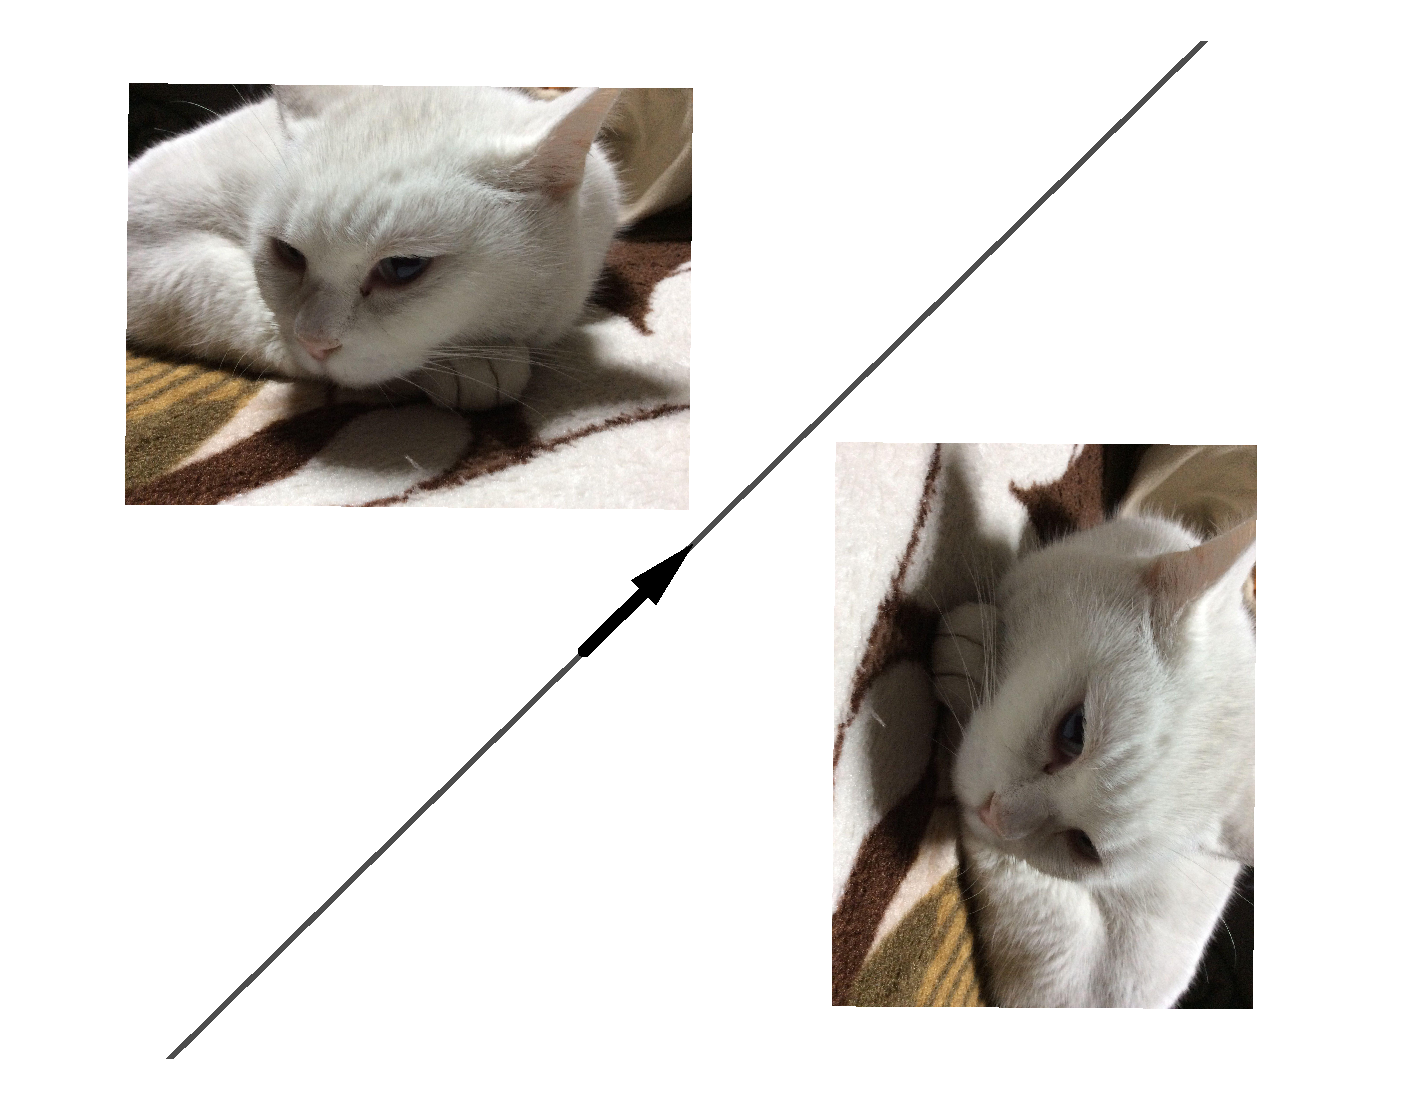
\includegraphics[height=10cm]{pictures/topoo.pdf}}
\maketitle
  


\section*{はじめに}

平面と空間の合同変換を線形代数をふんだんに使って分類してみました.はじ
めに合同変換を一般次元 $\mathbb{R}^n$ において定義しますが,過度に抽象
化はせず,平面 $\mathbb{R}^2$ と空間 $\mathbb{R}^3$(ついでに直
線 $\mathbb{R}$)の場合それぞれをできるだけ具体的に記述しました.平
面 $\mathbb{R}^2$ と空間 $\mathbb{R}^3$ の話は別々に読めるようになって
いるはずです.

 
 \newpage

 \section*{記号・記法}

\begin{itemize}
  \setlength{\itemsep}{1zh}

\item $\mathbb{R}^n$ を $n$ 次実列ベクトルのなす実線形空間とする.

\item 行列 $A$ の転置行列を ${}^{t}A$ で表す.
  
\item $\mathbb{R}^n$ の標準内積を $\cdot$ で表す.つまり,$\bm{x} \cdot \bm{y} = {}^{t}\bm{x} \bm{y}$ である.

\item $\mathbb{R}^n$ の標準内積から定まるノルムを $\| \; \|$ で表す.つ
  まり,$\|\bm{x}\| = \sqrt{\bm{x}\cdot \bm{x}}$ である.

\item 線形空間 $\mathbb{R}^n$ のゼロベクトルを $\bm{0}$ と書き,これを $\mathbb{R}^n$ の原点と
  も呼ぶ.
  
\item 線形空間の基底は順序付きの組として $(\bm{e}_1, \bm{e}_2, \ldots
  , \bm{e}_n)$ のように書く.例えば,$\mathbb{R}^3$
  の基底$(\bm{e}_1, \bm{e}_2, \bm{e}_3)$ と
  $(\bm{e}_1, \bm{e}_3, \bm{e}_2)$は別の基底として扱う.
  
\item $E$ を単位行列とし,次数 $n$ を明示したいときは $E_n$ と書く.

\item 行列 $A$ に対応する線形変換 $\bm{x}\mapsto A\bm{x}$ を $T_A$ で表す.

\item 正方行列 $A$ の固有値 $\lambda$ の固有空間を $V_A(\lambda)$ で表
  す.
\item $\mathbb{R}^n$ の部分線形空間 $V$ の直交補空間を $V^{\perp}$ で表す:
  \[
    V^{\perp} := \Set{\bm{x} \in \mathbb{R}^n | \text{ 任意の } \bm{y}
      \in V \text{ に対して } \bm{x}\cdot \bm{y}= 0}
  \]

\item 対角成分が左上から順に $a_1, \ldots, a_n$ である対角行列
  を $\diag(a_1, \ldots, a_n)$ で表す:
  \[
    \diag(a_1, a_2, \ldots, a_n) := \left[
      \begin{array}{ccc}
        a_1 & & O\\
         & \ddots &\\
        O & & a_n
      \end{array}
    \right]
  \]


\item 直交行列 $A,B$ が向きを保って同じ標準形に標準化されることを$ A \sim B$ で表す.
  \[
    A \sim B \overset{\textrm{def}}{\Longleftrightarrow} B= {}^{t}PAP \text{ か
      つ } \det(P) =1 \text{ となる直交行列 $P$ が存在する}
  \]

 
  
\end{itemize}

\newpage

\section{合同変換とは}\label{sec:whatis}

本節では $n$ を任意の自然数とするが,次節以降では $n$ を $2,3,1$ に固定する.

$\mathbb{R}^n$ を $n$ 次実列ベクトルのなす実線形空間とする.ま
た,$\bm{x}, \bm{y} \in
\mathbb{R}^n$に対して$\bm{x} \cdot \bm{y} := {}^{t}\bm{x} \bm{y}$ によっ
て内積を定める.さらに,$\| \bm{x}\| := \sqrt{\bm{x} \cdot \bm{x}}$ に
よってノルムを,$d(\bm{x}, \bm{y}) :=\|\bm{x} - \bm{y} \|$ よって距離を
定める.この距離 $d$ を保つ変換が合同変換である.つまり,合同変換は次のよう
に定義される.


\begin{definition}
  写像 $f:\mathbb{R}^n \to \mathbb{R}^n$
  が任意の$\bm{x}, \bm{y} \in \mathbb{R}^n$ に対して
  \[
    d(f(\bm{x}), f(\bm{y})) = d (\bm{x}, \bm{y}) \quad
    \Big( \Longleftrightarrow \;\|f(\bm{x}) - f(\bm{y})\| = \|\bm{x} - \bm{y}\| \Big)
  \]
  を満たすとき,$f$ を $\mathbb{R}^n$ の\textbf{合同変換}または\textbf{等長変換 (isometry)} という.
\end{definition}

\begin{remark}
  一般的な距離空間においては,距離を保つ全単射が等長写像(変換)と呼ば
  れる.合同変換という用語はユークリッド空間などのいくつかの特別な空間
  に対して使われるようである.また,上の定義では全単射性を仮定していな
  いが,$\mathbb{R}^n$ 上で距離 $d$ を保つ写像は全単射である.この事実
  は定理\ref{thm:affine_rep}から容易に導ける.
\end{remark}

\begin{theorem}\label{thm:trans-orth}
  \begin{enumerate}[(1)]
  \item ベクトル $\bm{b} \in \mathbb{R}^n$ による平行移
    動 $t_{\bm{b}}(\bm{x}) = \bm{x} + \bm{b}$ は $\mathbb{R}^n$ の合同変
    換である.
  \item 直交変換,すなわち,内積を保つ $\mathbb{R}^n$ の線形変換は合同
    変換である.
  \end{enumerate}
    \begin{proof}
      \begin{enumerate}[(1)]
      \item 任意の $\bm{x}, \bm{y}$ に対して
      \[
        \|t_{\bm{b}}(\bm{x}) - t_{\bm{b}}(\bm{y})\| =\|(\bm{x}+\bm{b}) -
        (\bm{y}+\bm{b})\| = \|\bm{x}-\bm{y}\|
      \]
      が成り立つので,$t_{\bm{b}}$ は $\mathbb{R}^n$ の合同変換である.
      
    \item $f$ を $\mathbb{R}^n$ の直交変換とする.$f$ は内積を保つので,
      任意の $\bm{x}, \bm{y} \in \mathbb{R}^n$ に対して
      \[
        \|f(\bm{x}) - f(\bm{y})\|^2 = \|f(\bm{x}-\bm{y})\|^2 = f(\bm{x}-\bm{y}) \cdot  f(\bm{x}-\bm{y})
        = (\bm{x}-\bm{y}) \cdot (\bm{x}-\bm{y}) = \|\bm{x}-\bm{y}\|^2
      \]
      が成り立つ.よって,$f$ は $\mathbb{R}^n$ の合同変換である.
    \end{enumerate}
  \end{proof}
\end{theorem}

合同変換と合同変換を合成するとやはり合同変換である.すなわち,次が成り立つ.

\begin{theorem}\label{thm:comp_isom}
  $\mathbb{R}^n$ の2つの合同変換の合成は $\mathbb{R}^n$ の合同変換である.
\end{theorem}

\begin{proof}
  $\mathbb{R}^n$ の合同変換 $f_1, f_2$ を任意にとる.任意の $\bm{x}, \bm{y} \in \mathbb{R}^n$ に対して
  \begin{align*}
    \|f_1 \left(f_2 \left(\bm{x}\right)\right)-f_1 \left(f_2\left(\bm{y}\right)\right)\|
    = \| f_2(\bm{x})- f_2(\bm{y}) \| = \|\bm{x}- \bm{y}\|
  \end{align*}
  が成り立つので,合成 $f_1 \circ f_2$ は $\mathbb{R}^n$ の合同変換である.
\end{proof}

\newpage

直交変換は線形変換なので原点 $\bm{0}$ を保つ合同変換である.この逆,すなわち,次が成り立つ.

\begin{theorem}\label{thm:prev0}
  原点 $\bm{0}$ を保つ合同変換は線形変換であり,従って,直交変換である.
\end{theorem}

\begin{proof}
  $f$ を $\mathbb{R}^n$ の合同変換とし,$f(\bm{0}) = \bm{0}$ とする.このとき,任
  意の $\bm{x} \in \mathbb{R}^n$ に対して
  \[
    \|f(\bm{x})\| = \|f(\bm{x})-\bm{0}\| =\|f(\bm{x})-f(\bm{0})\|  = \|\bm{x}-\bm{0}\| = \| \bm{x}\|
  \]
  が成り立つので,$f$ はノルムを保つ.これと内積とノルムの関係から任意
  の $\bm{x}, \bm{y} \in \mathbb{R}^n$ に対して
  \begin{align*}
    f(\bm{x})\cdot  f(\bm{y})
    &= \frac{1}{2}\left( \left\|f(\bm{x})\right\|^2+\left\|f(\bm{y})\right\|^2- \left\|f(\bm{x})-f(\bm{y})\right\|^2\right)\\
    & =\frac{1}{2}\left(\left\|\bm{x}\right\|^2+\left\|\bm{y}\right\|^2 - \left\|\bm{x}-\bm{y}\right\|^2\right)
      = \bm{x} \cdot  \bm{y}
  \end{align*}
  が成り立つので,$f$ は内積を保つ.以上から,任意の $\bm{x}, \bm{y}
  \in \mathbb{R}^n$ と任意の $k \in \mathbb{R}$ に対して
  \begin{align*}
    \left\|f(\bm{x}+\bm{y}) -  f(\bm{x}) - f(\bm{y}) \right\|^2
    =& \|f(\bm{x}+\bm{y})\|^2+\|f(\bm{x})\|^2+\|f(\bm{y})\|^2\\
     &- 2f(\bm{x}+\bm{y})\cdot  f(\bm{x})
       -2f(\bm{x}+\bm{y})\cdot  f(\bm{y}) +2f(\bm{x})\cdot f(\bm{y})\\
    =& \| \bm{x} + \bm{y}\|^2 + \|\bm{x}\|^2+\|\bm{y}\|^2\\
     &-2(\bm{x}+\bm{y})\cdot \bm{x} -2(\bm{x}+\bm{y})\cdot  \bm{y}+2\bm{x}\cdot \bm{y}\\
    =& \|\bm{x}+\bm{y} - \bm{x}-\bm{y}\|^2=\|\bm{0}\|^2=0,\\
    \left\| f(k\bm{x}) - k f(\bm{x})\right\|^2  
    =& \|f(k\bm{x})\|^2-2 f(k\bm{x})\cdot kf(\bm{x}) + \|kf(\bm{x})\|^2\\
    =& \|k\bm{x}\|^2 - 2k \left(f(k\bm{x})\cdot f(\bm{x}) \right)+ k^2\|f(\bm{x})\|^2\\
    =& \|k\bm{x}\|^2-2k\left( k\bm{x}\cdot  \bm{x}\right) + k^2 \|\bm{x}\|^2=0
  \end{align*}
  が成り立つ.よって,$f$ は線形変換である.さらに,$f$ は内積を保つの
  で直交変換である.
\end{proof}

この定理から,任意の合同変換は直交行列とベクトルによって表せる.すなわち,次が成り立つ.

\begin{theorem}\label{thm:affine_rep}
  $\mathbb{R}^n$ の任意の合同変換 $f$ は,$n$ 次直交行列 $A$
  と $n$ 次ベクトル $\bm{b} \in \mathbb{R}^n$ によって
  \[
    f(\bm{x}) = A\bm{x} + \bm{b}
  \]
  と一意的に表せる.逆に,この形で表せる写像は $\mathbb{R}^n$ の合同変換である.
\end{theorem}


\begin{proof}
  $f$ を $\mathbb{R}^n$ の任意の合同変換とする.$f(\bm{0})=\bm{b}$ とお
  く.定理\ref{thm:trans-orth}(1)と定
  理\ref{thm:comp_isom}よりベクトル $-\bm{b}$ による平行移
  動 $t_{-\bm{b}}$ と $f$ の合成 $g = t_{-\bm{b}} \circ
  f$ は $\mathbb{R}^n$ の合同変換である.$g(\bm{0})=\bm{0}$ なので,定
  理\ref{thm:prev0}より $g$は直交変換である.従って,ある $n$ 次直交行
  列 $A$
  によって$g(\bm{x})=A\bm{x}$と表せる.よって,$f(\bm{x}) =
  g(\bm{x})+\bm{b} = A\bm{x} + \bm{b}$である.また,
  \[
    f(\bm{x}) = A\bm{x}+\bm{b} = B\bm{x} + \bm{c}
  \]
  と表せたとすると,$f(\bm{0})=\bm{b}=\bm{c}$ である.従って,$f$ に対
  して直交変換 $g$ が一意的に定まるので,対応する直交行列も一意的に定ま
  るから $A=B$ である.後半の主張は明らかである.
\end{proof}

\newpage

\section{平面の合同変換}\label{sec:2dim}

平面は $\mathbb{R}^2$ と同一視し,平面ベクトルを以下のように $2$ 次列ベクトルとして書く.
\[
  \bm{x} = \left[
  \begin{array}{c}
    x_1\\
    x_2
  \end{array}
\right], \quad \bm{y}= \left[
  \begin{array}{c}
    y_1\\
    y_2
  \end{array}
\right] 
\]
幾何学的にはこれらを平面の点として $\bm{x}=(x_1,x_2), \;
\bm{y}=(y_1,y_2)$ ともみなしつつ,代数的に $2$ 次列ベクトルとして扱っていく.
平面 $\mathbb{R}^2$ における内積とノルムは具体的に以下のように書ける.
\[
  \bm{x} \cdot  \bm{y} = {}^{t}\bm{x} \bm{y} = \left[
    \begin{array}{cc}
      x_1 & x_2
    \end{array}
  \right] \left[
    \begin{array}{c}
      y_1\\
      y_2
    \end{array}
  \right] = x_1 y_1 + x_2 y_2, \quad \| \bm{x} \| = \sqrt{\bm{x} \cdot \bm{x}} = \sqrt{x_1^2+x_2^2}
\]


以下,$f$ を平面 $\mathbb{R}^2$ の合同変換とする.定理\ref{thm:affine_rep}か
ら $2$ 次直交行列 $A$ と平面ベクトル $\bm{b} \in \mathbb{R}^2$ によって
\[
  f(\bm{x}) = A\bm{x} + \bm{b}
\]
と書ける.この表示をもとに,$f$ を分類していく.

\subsection{固定点集合}\label{sec:inv2}

合同変換 $f$ はその固定点集合によって特徴づけられ
る.$f(\bm{x})=\bm{x}$ を満たす $\bm{x} \in \mathbb{R}^2$ を $f$ の固定
点という.$f$ の固定点集合
\[
  \Fix(f) := \Set{ x \in \mathbb{R}^2 | f(\bm{x}) = \bm{x}} \subset \mathbb{R}^2
\]
が平面上でどのような図形になるかを考えよう.
\[
  f(\bm{x}) = \bm{x} \Leftrightarrow A\bm{x} + \bm{b} = \bm{x} \Leftrightarrow (E-A)\bm{x} = \bm{b}
\]
なので,$\Fix(f)$ は $2$ 変数連立1次方程式 $(E-A)\bm{x} = \bm{b}$
の解全体のなす集合である.従って,$\Fix(f)$ は空集合,$1$ 点集合,直線,
平面全体のいずれかである.特に,$f$ が恒等変換のとき,またそのときに限
り,$\Fix(f)=\mathbb{R}^2$ となる.すなわち,
\[
  A=E \text{ かつ } \bm{b} = \bm{0} \Leftrightarrow f =
  \id_{\mathbb{R}^2} \Leftrightarrow \Fix(f) = \mathbb{R}^2
\]
である.また,
\[
  A=E \text{ かつ } \bm{b} \neq \bm{0} \Rightarrow \Fix(f) = \emptyset
\]
である.すなわち,$\bm{0}$ でないベクトル $\bm{b}$ による平行移
動 $t_{\bm{b}}$ は固定点を持たない.

$A$ が $1$ を固有値に持たないとき,$\det(E-A) \neq 0$ だから $E-A$ は正
則である.従って,このとき連立 $1$ 次方程式 $(E-A)\bm{x} = \bm{b}$ は唯
一つの解 $\bm{x} = (E-A)^{-1}\bm{b}$ を持つから,$\Fix(f)$ は $1$ 点集
合である.すなわち,以下が成り立つ.
\[
  \text{ $1$ は $A$ の固有値でない } \Rightarrow \Fix(f) =
  \Set{(E-A)^{-1}\bm{b}}
\]

$A$ が $1$ を固有値に持つとき,その固有空間 $V_A(1)$ は同次形連立 $1$
次方程式 $(E-A)\bm{x}=\bm{0}$ の解空間に等しい.さらに,連立 $1$ 次方程
式 $(E-A)\bm{x}=\bm{b}$ が解を持つなら,その一般解は特殊解 $\bm{x}_0$
を用いて$\bm{x} = \bm{x}_0 + \bm{x}_1 \; (\bm{x}_1 \in V_A(1))$ と書け
る.すなわち,
\[
  \text{ $1$ が $A$ の固有値かつ } \Fix(f) \neq \emptyset \Rightarrow
  \Fix(f) = \Set{\bm{x}_0 +  \bm{x}_1 | \bm{x}_1 \in V_A(1)}
\]
である.特に,$\dim V_A(1) = 1$ なら $\Fix(f)$ は $\bm{x}_0$ を通
り $V_A(1)$ に平行な直線である.なお,連立 $1$ 次方程
式 $(E-A)\bm{x}=\bm{b}$ が解を持たければ,$\Fix(f)$ は空集合である.


\subsection{平面の直交変換}

よく知られているように,$2$ 次直交行列は以下のどちらか一方の形に書ける.
\[
  S_{\theta} := \left[
    \begin{array}{rr}
      \cos\theta & -\sin\theta\\
      \sin\theta & \cos\theta
    \end{array}
  \right], \quad R_{\theta} :=\left[
    \begin{array}{rr}
      \cos\theta & \sin\theta\\
      \sin\theta & -\cos\theta
    \end{array}
  \right] \quad (\theta \in \mathbb{R})
\]
$S_{\theta}$ に対応する直交変換は図\ref{fig:rotaion2}のように原点を中心
とする角度 $\theta$ の回転であり,$R_{\theta}$ に対応する直交変換は
図\ref{fig:reflection2}のように原点で $x$ 軸と角度 $\frac{\theta}{2}$
で交わる直線に関する鏡映である.ただし,角度は反時計回りを正の向きとす
る.
\begin{figure}[h]
  \centering
  \begin{tabular}{c}
    \begin{minipage}{0.45\linewidth}
      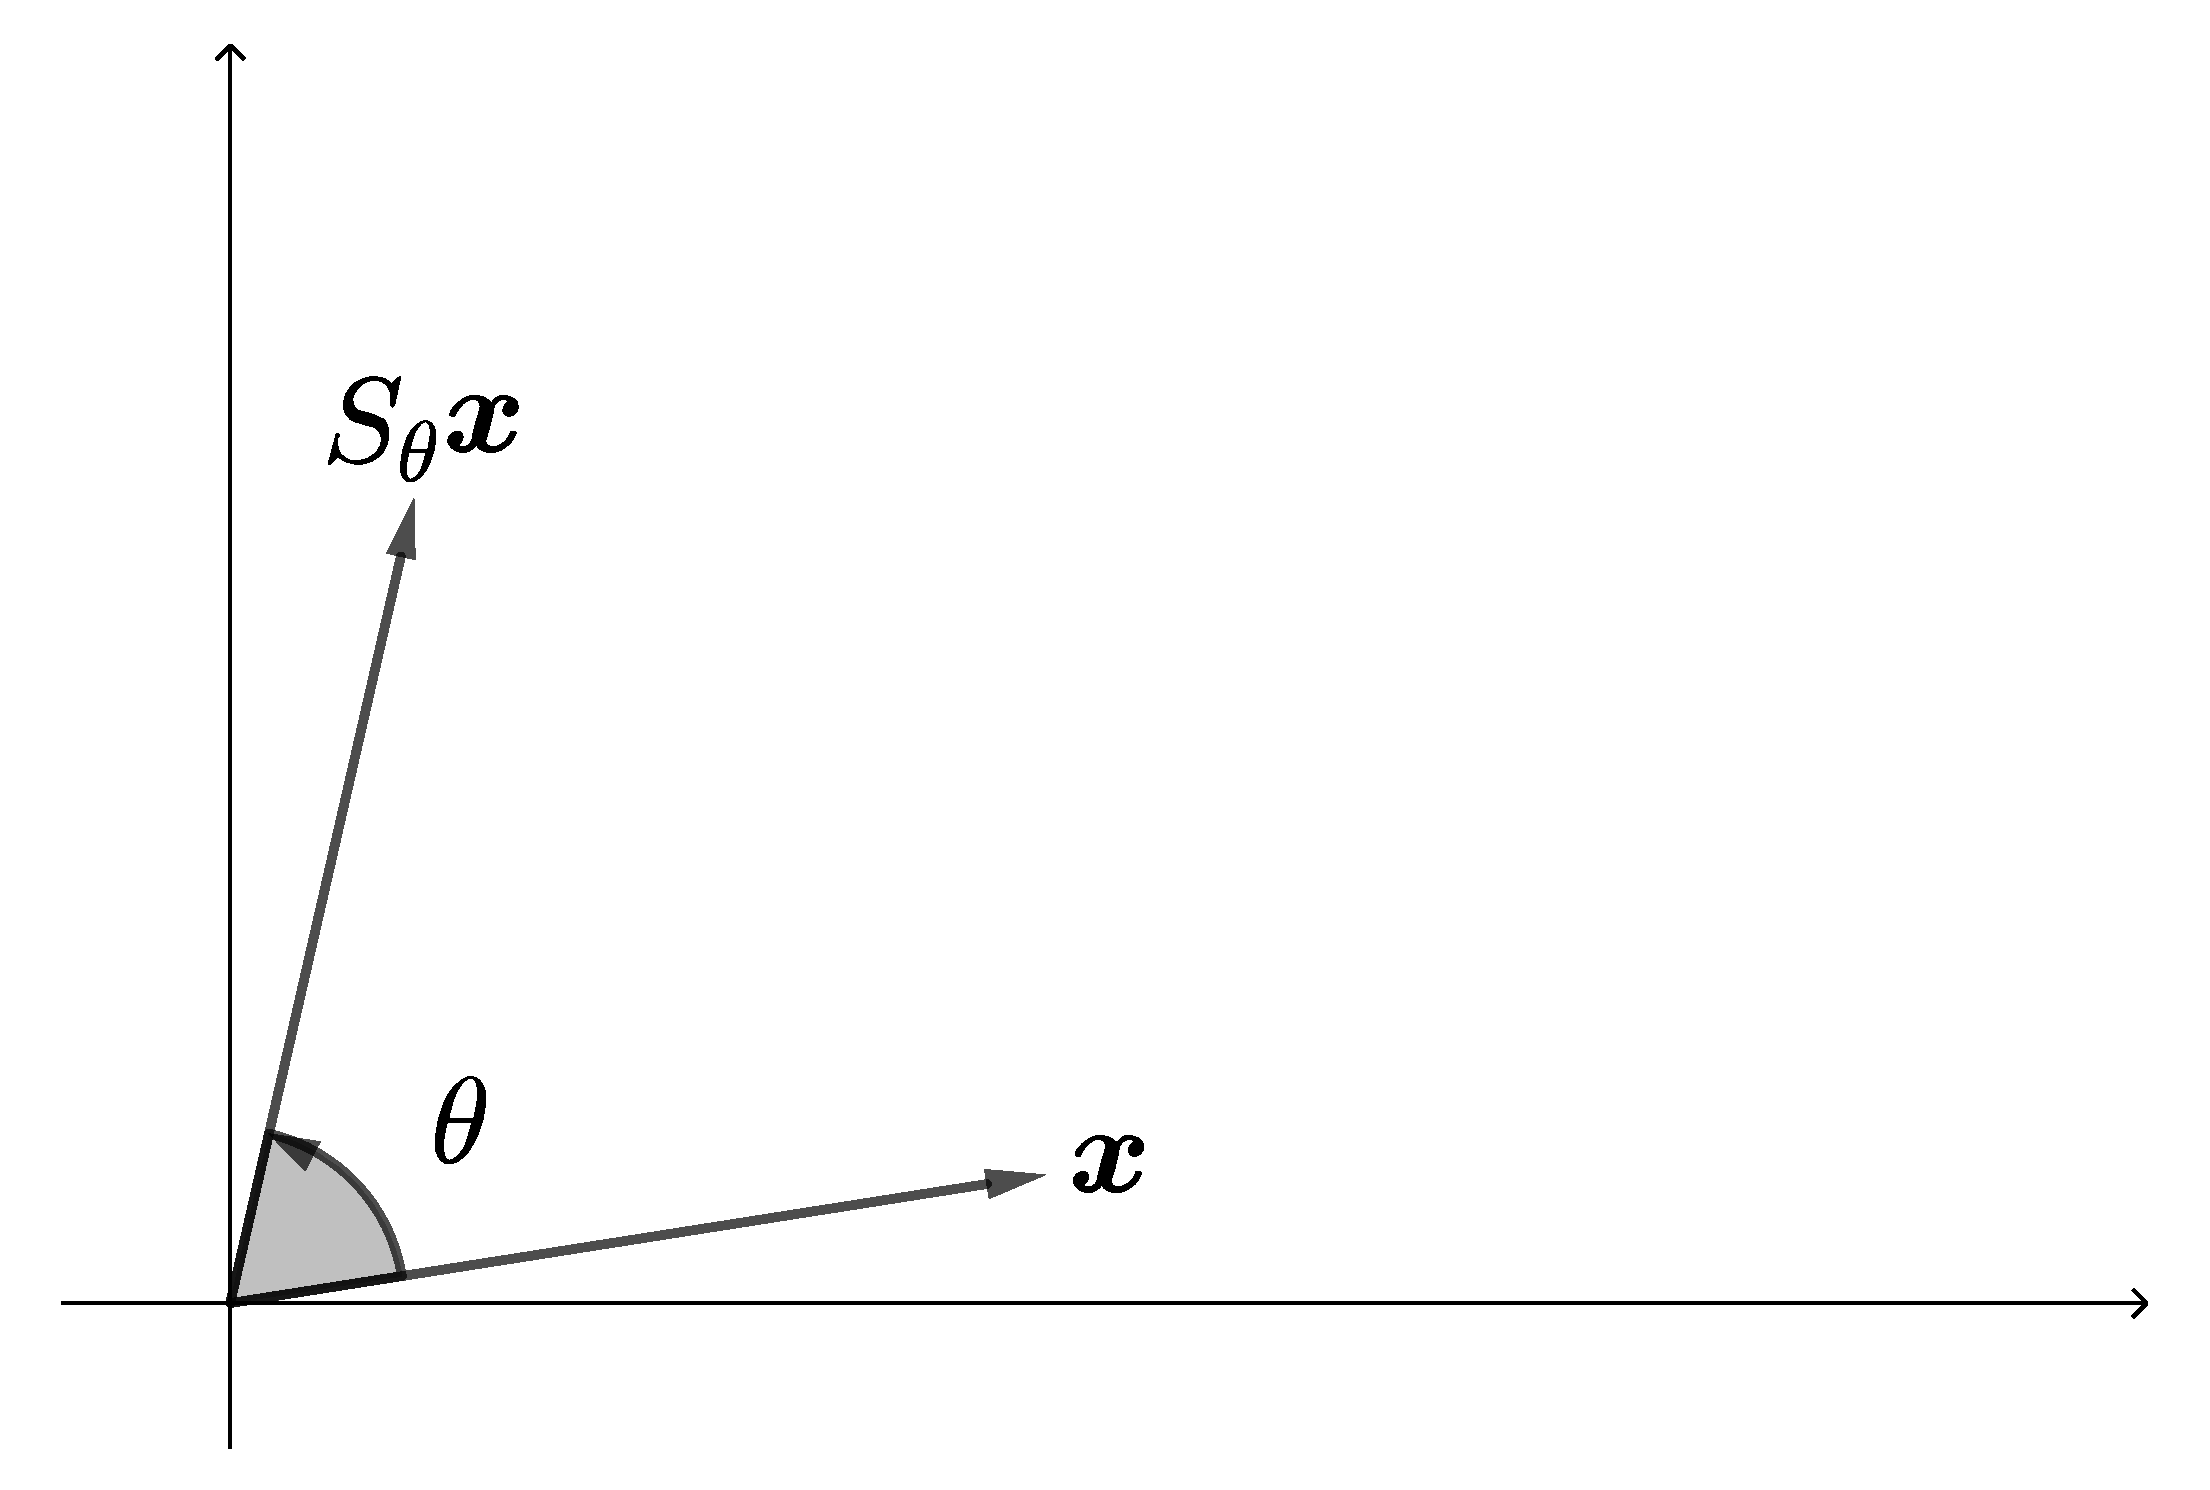
\includegraphics[height=4.5cm]{pictures/rotation2.pdf}
      \caption{原点を中心とする$\theta$ 回転}\label{fig:rotaion2}
    \end{minipage}
    \begin{minipage}{0.45\linewidth}
    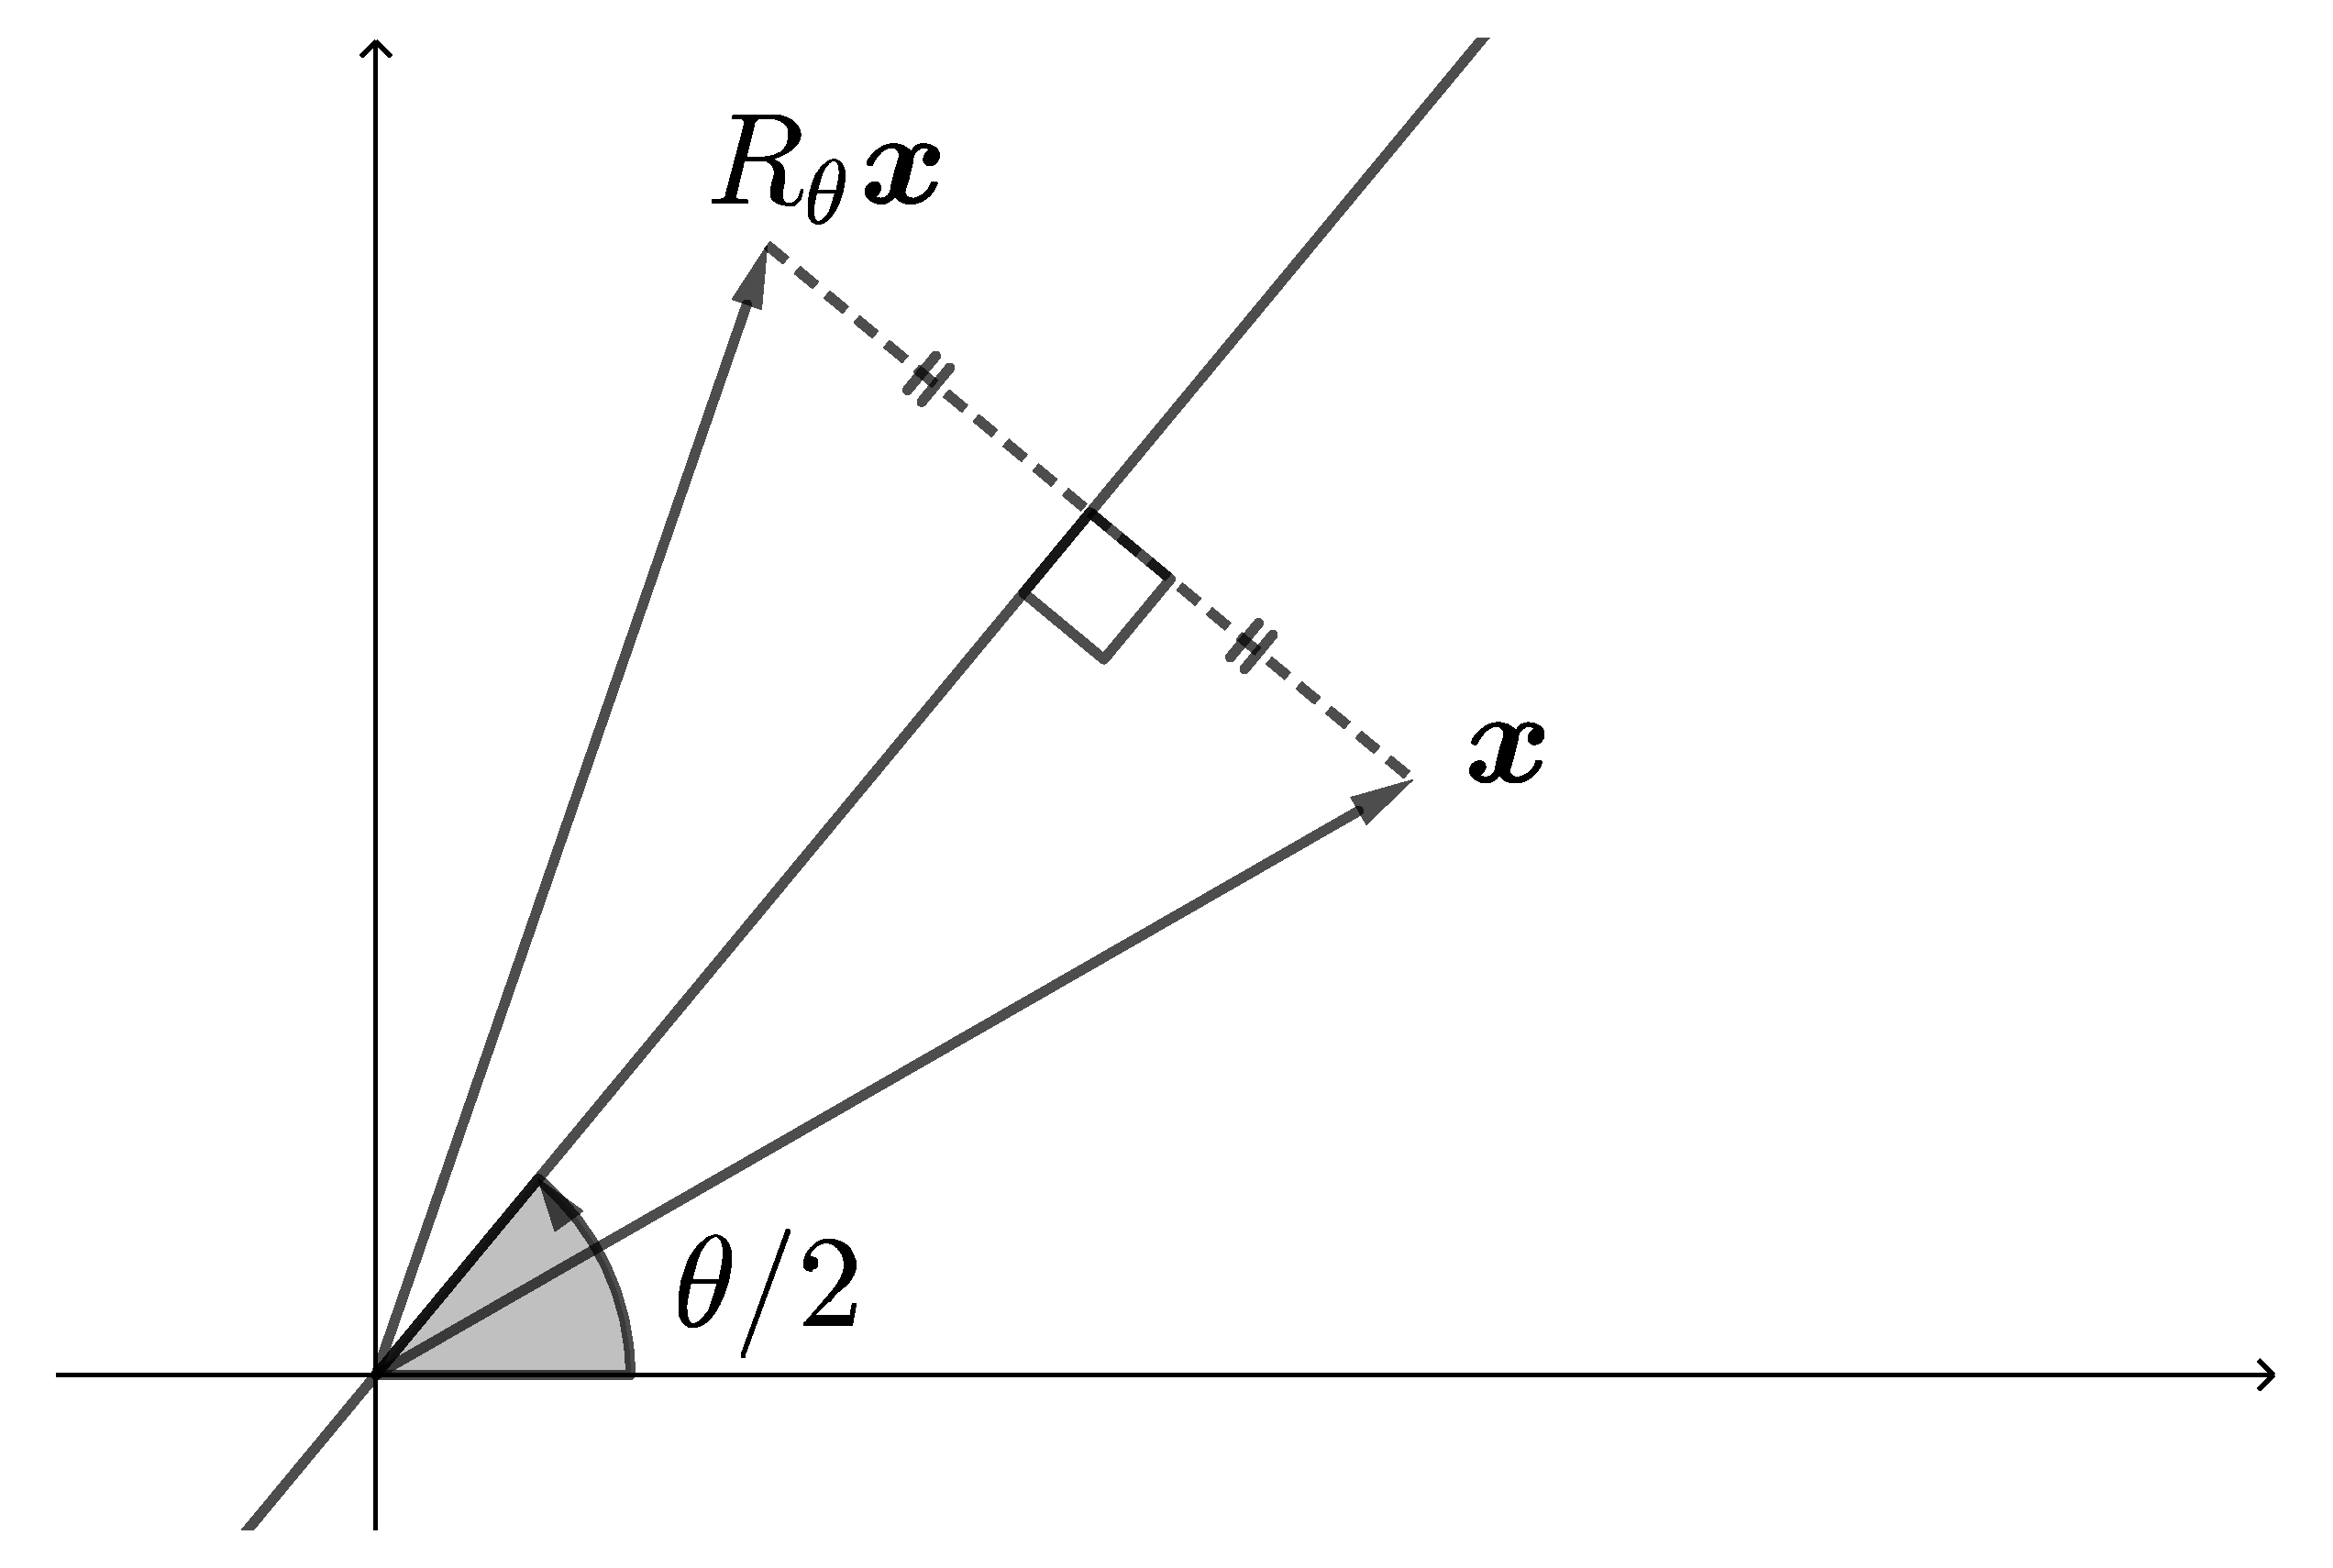
\includegraphics[height=4.5cm]{pictures/reflection2.pdf}
    \caption{原点で $x$ 軸と$\theta/2$ で交わる直線に関する鏡映}\label{fig:reflection2}      
    \end{minipage}
  \end{tabular}
\end{figure}

$2$ 次直交行列全体の集合を $O(2)$ と書く.また,$SO(2) := \Set{A \in
  O(2) | \det A = 1}$ とする.$\det S_{\theta} =1, \; \det
R_{\theta}=-1$ であり,直交行列の行列式は $\pm 1$ だから,
\[
  SO(2) = \Set{ S_{\theta} | \theta \in \mathbb{R}}, \quad O(2)
  \setminus SO(2)=\Set{ R_{\theta} | \theta \in \mathbb{R}}
\]
である.回転同士,鏡映同士の合成は回転であり,回転と鏡映の合成は鏡映である.具体的には
\[
  S_{\theta} S_{\phi} = S_{\theta+\phi}, \quad R_{\theta} R_{\phi} = S_{\theta-\phi}, \quad
  S_{\theta}R_{\phi}=R_{\theta+\phi}, \quad R_{\theta}S_{\phi} = R_{\theta-\phi}
\]
である.特に,$S_{\theta} = R_{\theta}R_{0}, R_{\theta}^2=E$ である.さらに,
\[
  S_{\frac{\theta}{2}}^{-1} R_{\theta} S_{\frac{\theta}{2}} = S_{-\frac{\theta}{2}} R_{\theta} S_{\frac{\theta}{2}}
  = R_{0} = \left[
    \begin{array}{rr}
      1 & 0\\
      0 & -1
    \end{array}
  \right]
\]
より,$R_{\theta}$ は $S_{\frac{\theta}{2}}$ により直交対角化されることがわかる.これより(あるいは直接的な計算により)
$R_{\theta}$ の固有値は $1, -1$ で,各々の固有空間 $V_{R_{\theta}}(1), V_{R_{\theta}}(-1)$ は互いに直交し,
\[
  V_{R_{\theta}}(1) = \left\langle \left[
    \begin{array}{r}
      \cos (\theta/2)\\
      \sin (\theta/2)
    \end{array}
  \right]\right\rangle, \quad V_{R_{\theta}}(-1)= \left\langle \left[
    \begin{array}{r}
      -\sin (\theta/2)\\
      \cos (\theta/2)
    \end{array}
  \right]\right\rangle
\] 
であることもわかる.なお,$V_{R_{\theta}}(1)$ が鏡映の軸である.ま
た,$S_0, S_{\pi}$ 以外の $S_{\theta}$ は実固有値を持たない.


\subsection{平面の合同変換の分類}\label{sec:classification2}

平面 $\mathbb{R}^2$ の合同変換
\[
  f(\bm{x}) = A \bm{x} + \bm{b}
\]
は直交行列 $A$ と $2$ 次列ベクトル $\bm{b}$ によって
表\ref{tab:classification2}のように $5$ 種に分類できる.定
理\ref{thm:generate2}で示すように,平面の合同変換は $3$ 個以下の鏡映の
合成として表せる.表\ref{tab:classification2}の $4$ 列目はその鏡映の最
小個数を表している.

\begin{table}[h]
  \centering
  \begin{tabular}[h]{|c|c|c|c|c|}\hline
    名前 & $A$ & $\bm{b}$ & 鏡映の最小個数 & 固定点集合\\ \hline
    恒等変換 & $E$ & $\bm{0}$ & $0$ & $\mathbb{R}^2$ \\
    平行移動 & $E$ & $\bm{b} \neq \bm{0}$ & $2$ & 空集合\\
    回転 & $S_{\theta} (\neq E$) & $\bm{b} \in \mathbb{R}^2$ & $2$ & 回転の中心\\
    鏡映 & $R_{\theta}$ & $\bm{b} \in V_{R_{\theta}}(-1)$ & $1$ & 鏡映軸  \\
    滑り鏡映 & $R_{\theta}$ & $\bm{b} \notin V_{R_{\theta}}(-1)$ & $3$ & 空集合\\ \hline
  \end{tabular}
  \caption{平面 $\mathbb{R}^2$ の合同変換の分類表}
  \label{tab:classification2}
\end{table}


ここでは,実際に平面 $\mathbb{R}^2$ の合同変
換 $f$ が表\ref{tab:classification2}のいずれかに分類され,またそれで全
てであることを確かめていこう.恒等変換と平行移動に関しては明らかなので,
以下 $f$ は恒等変換でも平行移動でもない,すなわち,$A \neq E$ とする.
また,直交行列 $S_{\theta}, R_{\theta}$ に対応する直交変換をそれぞ
れ $s_{\theta}, r_{\theta}$ で表す.なお,恒等変換は本来平行移動及び回
転の一種ではあるが,本稿では分類の都合上平行移動とも回転とも
別のクラスとして扱う.

\subsubsection{回転}\label{sec:rotation2}

$A = S_{\theta} \in SO(2) \; (S_{\theta} \neq E)$ とする.このとき $f$ の固
定点は1点のみであり,$f$ はその固定点を中心とする $\theta$ 回転である.
このことを実際に確かめてみよう.

$S_{\theta}$ は $1$ を固有値に持たないので,$\det(E-S_{\theta}) \neq
0$ である.従って,$E-S_{\theta}$ は正則なので
\[
  \bm{x} \in \Fix(f) \Leftrightarrow S_{\theta} \bm{x} +\bm{b} =
  \bm{x} \Leftrightarrow (E-S_{\theta})\bm{x} = \bm{b} \Leftrightarrow
  \bm{x} = \left( E-S_{\theta}\right)^{-1} \bm{b}
\]
である.従って,$f$ の固定点
は $\bm{c}:=\left(E-S_{\theta}\right)^{-1}\bm{b}$ のみである.このとき,
任意の $\bm{x} \in \mathbb{R}^2$ に対して
\[
  f(\bm{x}) - \bm{c} = S_{\theta}(\bm{x}-\bm{c})
\]
である.よって,確かに $f$ は $\bm{c}$ を中心とする $\theta$ 回転である
ことがわかる(図\ref{fig:rotation2gen}).また,これより
\[
  f = t_{\bm{c}} \circ s_{\theta} \circ t_{-\bm{c}}
\]
とも表せる.すなわち,$\bm{c}$ を中心とする回転は「一旦 $-\bm{c}$ 平行
移動し,原点を中心に回転させた後に再び $\bm{c}$ 平行移動する変換」と言
い換えることもできる.
\begin{figure}[h]
  \centering
  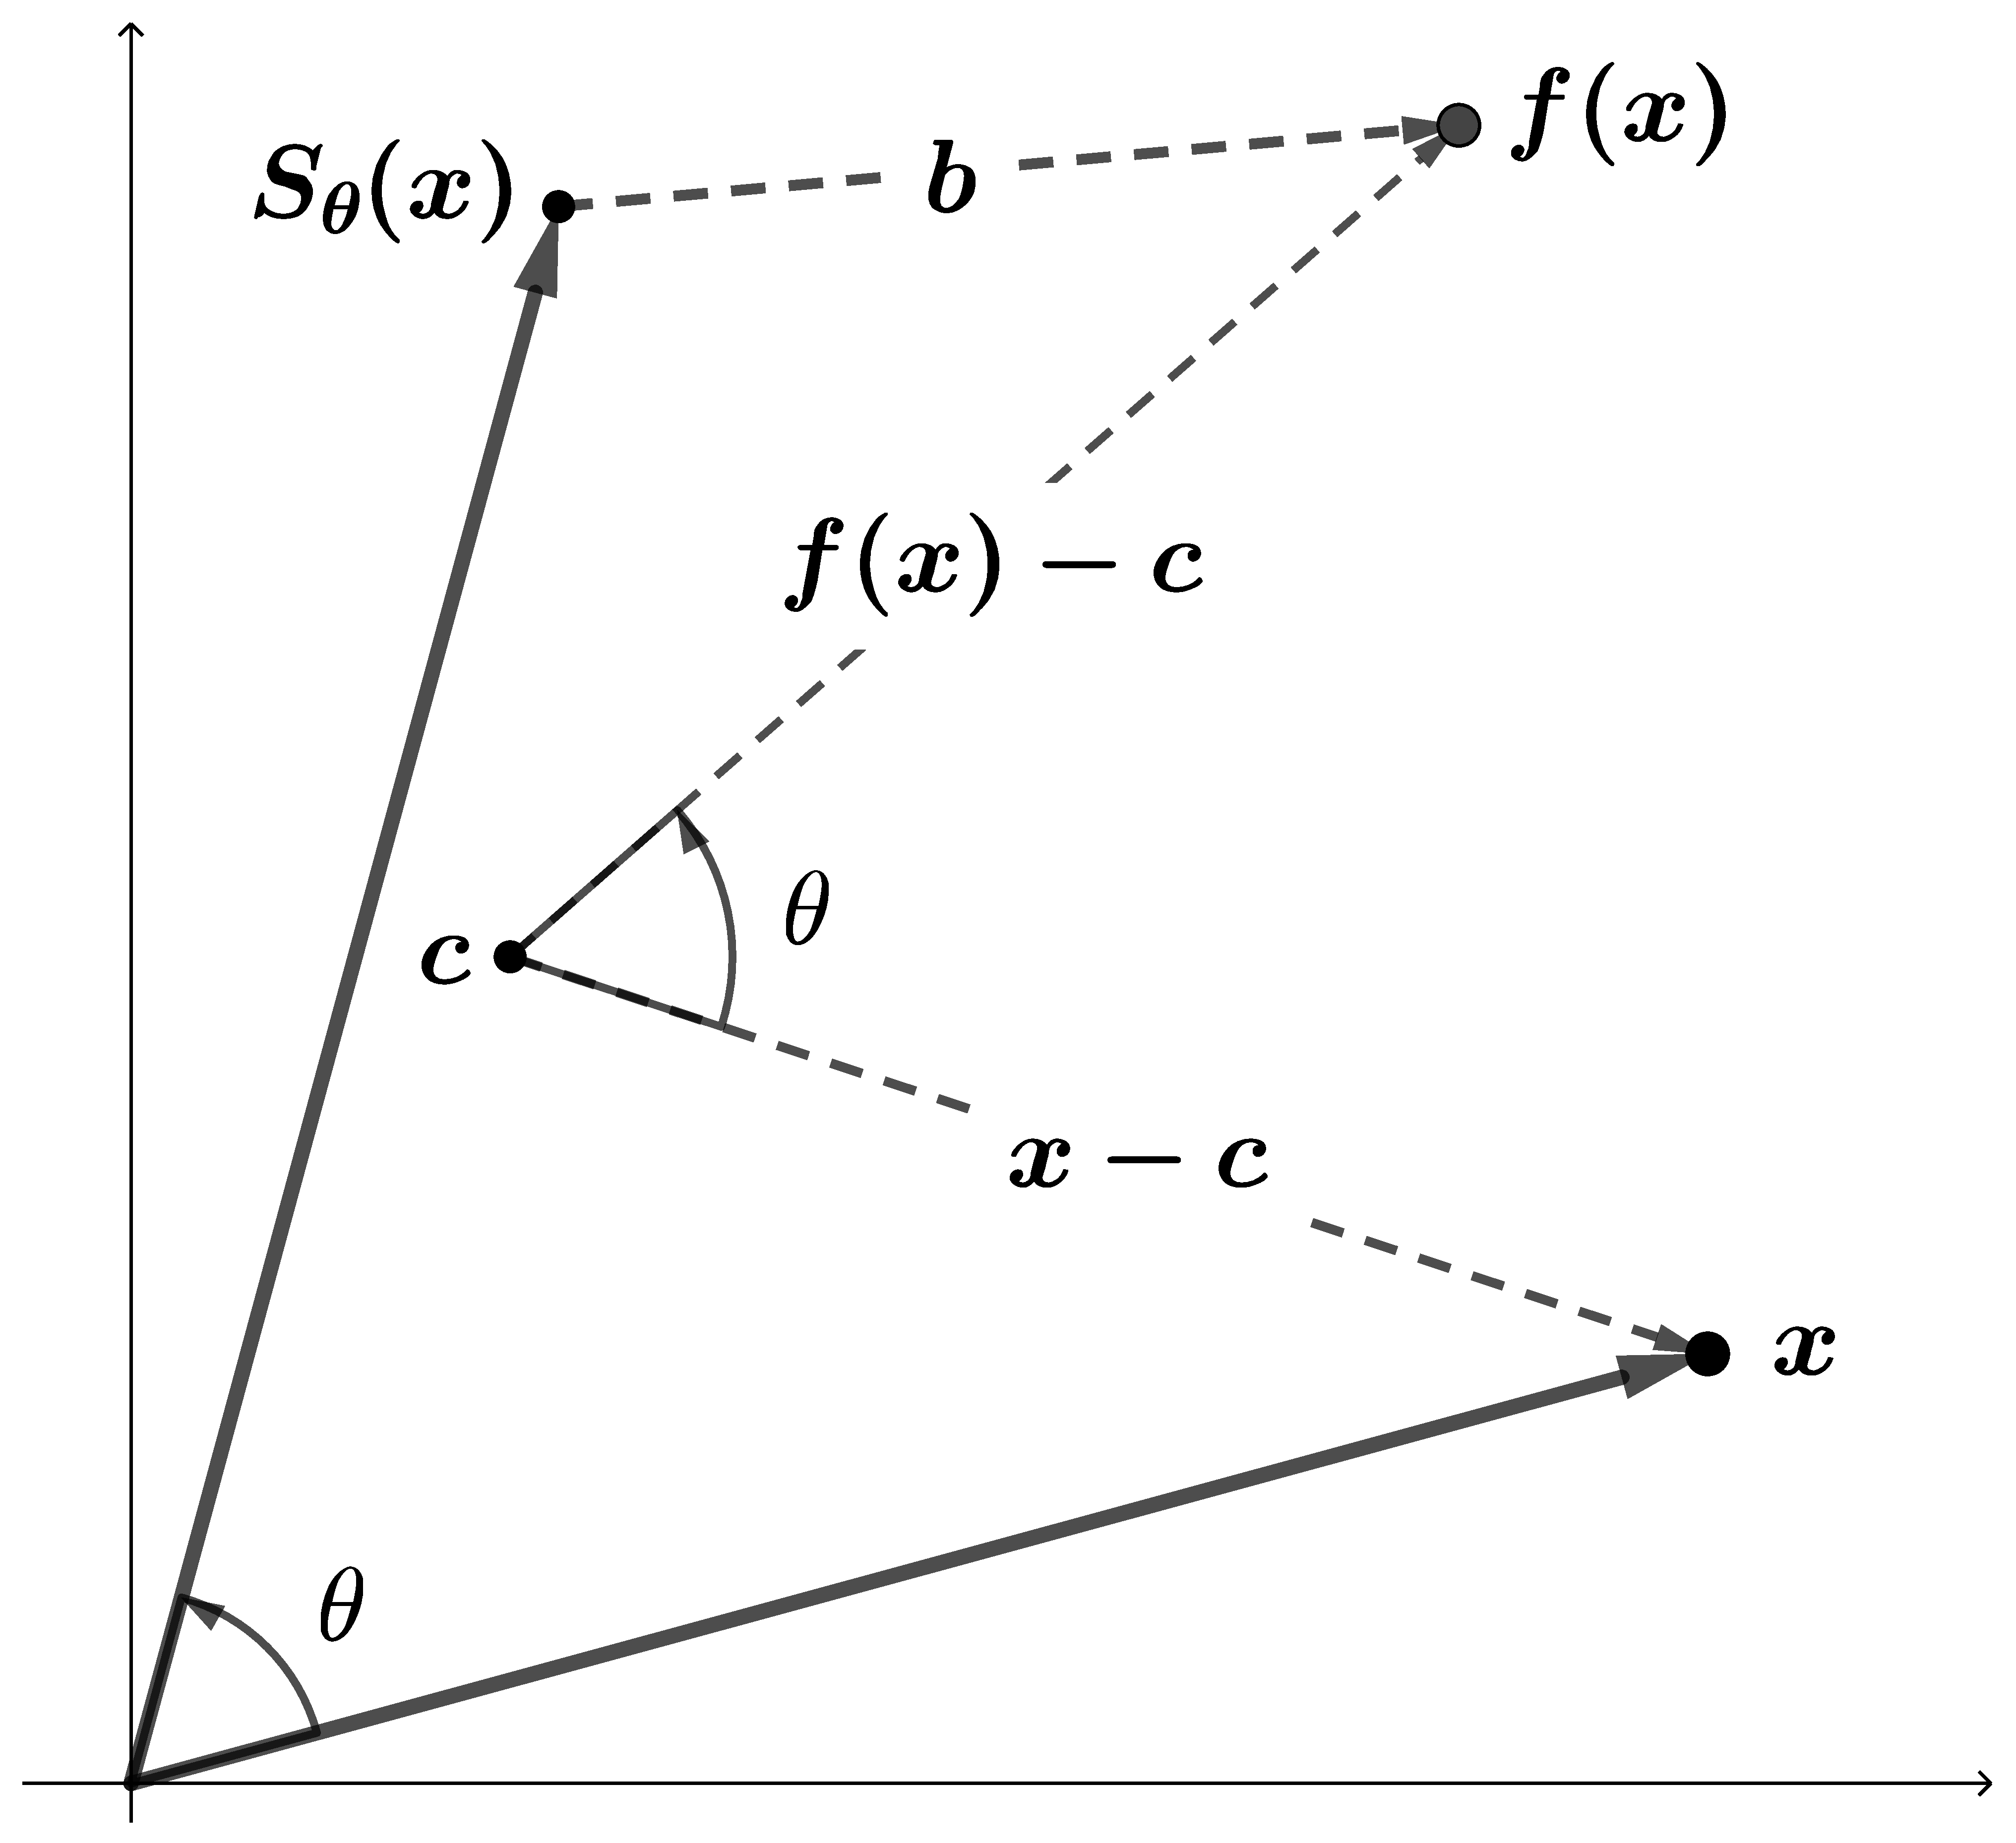
\includegraphics[height=5cm]{pictures/rotation2gen.pdf}
  \caption{$\bm{c}$ を中心とする $\theta$ 回転}
  \label{fig:rotation2gen}
\end{figure}


\subsubsection{鏡映と滑り鏡映}\label{sec:reflection2}

$A=R_{\theta} \in O(2) \setminus SO(2)$
とする.このとき,$\bm{b} \in
V_{R_{\theta}}(-1)$ なら $\Fix(f)$ は $\bm{b}/2$ を通り $V_{R_{\theta}}(1)$ に
平行な直線であり,$f$ はこの直線に関する鏡映である.一方,$\bm{b}
\notin V_{R_{\theta}}(-1)$ なら $\Fix(f)$ は空集合であり,$f$ は滑り鏡映で
ある.これを実際に確かめていこう.

直交行列 $R_{\theta}$ による固有空間分解
$\mathbb{R}^2 = V_{R_{\theta}}(1) \oplus V_{R_{\theta}}(-1)$ によって $\bm{b}$
を
\begin{equation}\label{eq:eigendecomp2}
  \bm{b} = \bm{b}^{+} + \bm{b}^{-}, \quad \bm{b}^{+} \in V_{R_{\theta}}(1), \; \bm{b}^{-} \in V_{R_{\theta}}(-1)
\end{equation}
と分解する.ここで,$\Fix(f) \neq \emptyset$ とすると,$x \in \Fix(f)$
に対して $f(\bm{x}) = {x}$ なので
\begin{equation}\label{eq:xinInv}
  R_{\theta}x +\bm{b}^{+} + \bm{b}^{-} = \bm{x}
\end{equation}
である.この式 (\ref{eq:xinInv}) の両辺に $R_{\theta}$ を左から掛ける
と,$R_{\theta}^2=E, \; R_{\theta} \bm{b}^{\pm} = \pm \bm{b}^{\pm}$ なので
\begin{equation}\label{eq:RxinInv}
  \bm{x}+\bm{b}^{+}-\bm{b}^{-}=R_{\theta}\bm{x} 
\end{equation}
が得られる.これら (\ref{eq:xinInv}) と (\ref{eq:RxinInv}) から $b^{+}
= \bm{0}$ より,$\bm{b} \in V_{R_{\theta}}(-1)$
である.逆に,$\bm{b} \in V_{R_{\theta}}(-1)$ とすると,$R_{\theta}\bm{b}
= -\bm{b}$ なので
\begin{equation}\label{eq:halfinInv}
  f\left(\frac{\bm{b}}{2}\right) = R_{\theta}\left(\frac{b}{2}\right) + \bm{b}
  = -\frac{\bm{b}}{2}+\bm{b} = \frac{\bm{b}}{2}
\end{equation}
より,$\bm{b}/2 \in \Fix(f)$ だから $\Fix(f) \neq \emptyset$ である.以上から,
\[
  \Fix(f) \neq \emptyset \Leftrightarrow \bm{b} \in V_{R_{\theta}}(-1)
\]
である.これにより,$\bm{b} \in V_{R_{\theta}}(-1)$ かそうでないかによって合
同変換 $f$ を分けることができる.


初めに,$\bm{b} \in V_{R_{\theta}}(-1)$ とする.このとき $\Fix(f)$ は直線
で,$f$ がこの直線 $\Fix(f)$ に関する鏡映であることを確かめよう.

ま
ず,$\Fix(f)$ が直線となることを確かめておく.$\Fix(f)$ が空集合でない
ので,連立 $1$ 次方程式
\[
  (E-R_{\theta})\bm{x} = \bm{b}
\]
は解を持つ.$R_{\theta}$ は $1$ を固有値に持つので $\det
(E-R_{\theta}) = 0$ であり,$E-R_{\theta} \neq O$ だか
ら,$\rank(E-R_{\theta})=1$ である.従って,$\dim V_{R_{\theta}}(1)=1$ なの
で \ref{sec:inv2}節で見たように $\Fix(f)$ は直線である.特に,(\ref{eq:halfinInv})
より $\bm{b}/2 \in \Fix(f)$ だから $\Fix(f)$ は $\bm{b}/2$ を通る.さら
に,任意の $\bm{x} \in \Fix(f)$ に対して,
\[
  \bm{x} \cdot \bm{b} = (R_{\theta}\bm{x}) \cdot  (R_{\theta}\bm{b}) =
  (\bm{x}-\bm{b})\cdot (-\bm{b}) = -\bm{x}\cdot \bm{b}+\|\bm{b}\|^2
\]
より $(\bm{x}, \bm{b}) = \|\bm{b}\|^2/2$
が成り立つから$\left( \bm{x}-\bm{b}/2\right) \cdot  \bm{b}=0$ とな
り,$\Fix(f)$ と $\bm{b}$ は直交する.つま
り,$\Fix(f)$ は $V_{R_{\theta}}(-1)^{\perp}=V_{R_{\theta}}(1)$ に平行
で $\bm{b}/2$ を通る直線である.

次に,実際に $f$ が直線 $\Fix(f)$ に関する鏡映であることを確かめる.任
意の $\bm{x} \in \mathbb{R}^2$ と任意の $\bm{p} \in V_{R_{\theta}}(1)$ に対
して,
\begin{align*}
  \left( f\left(\bm{x}\right) - \bm{x}\right) \cdot  \bm{p}
  &= (R_{\theta}\bm{x}) \cdot  \bm{p} +\bm{b}\cdot \bm{p}- \bm{x} \cdot \bm{p}
    =(R_{\theta}\bm{x}) \cdot  (R_{\theta}\bm{p})-\bm{x}\cdot \bm{p}
    =\bm{x} \cdot \bm{p} - \bm{x} \cdot  \bm{p}=0,\\
  f\left(\frac{f(\bm{x})+\bm{x}}{2}\right) 
  &= R_{\theta}\left(
    \frac{R_{\theta}\bm{x} + \bm{b} + \bm{x}}{2}\right) + \bm{b}
    =\frac{\bm{x}-\bm{b}+R_{\theta}\bm{x}}{2} + \bm{b}
    =\frac{R_{\theta}\bm{x}+\bm{b} + \bm{x}}{2} = \frac{f(\bm{x})+\bm{x}}{2}
\end{align*}
であるから,$f(\bm{x})-\bm{x}$ が $V_{R_{\theta}}(1)$ に,従っ
て $\Fix(f)$に,直交し,$f(\bm{x})$ と $\bm{x}$ の中点が $\Fix(f)$ 上に
あるので,$f$ は確かに直線 $\Fix(f)$ に関する鏡映である(
図\ref{fig:reflection2gen}).
\begin{figure}[h]
  \centering
  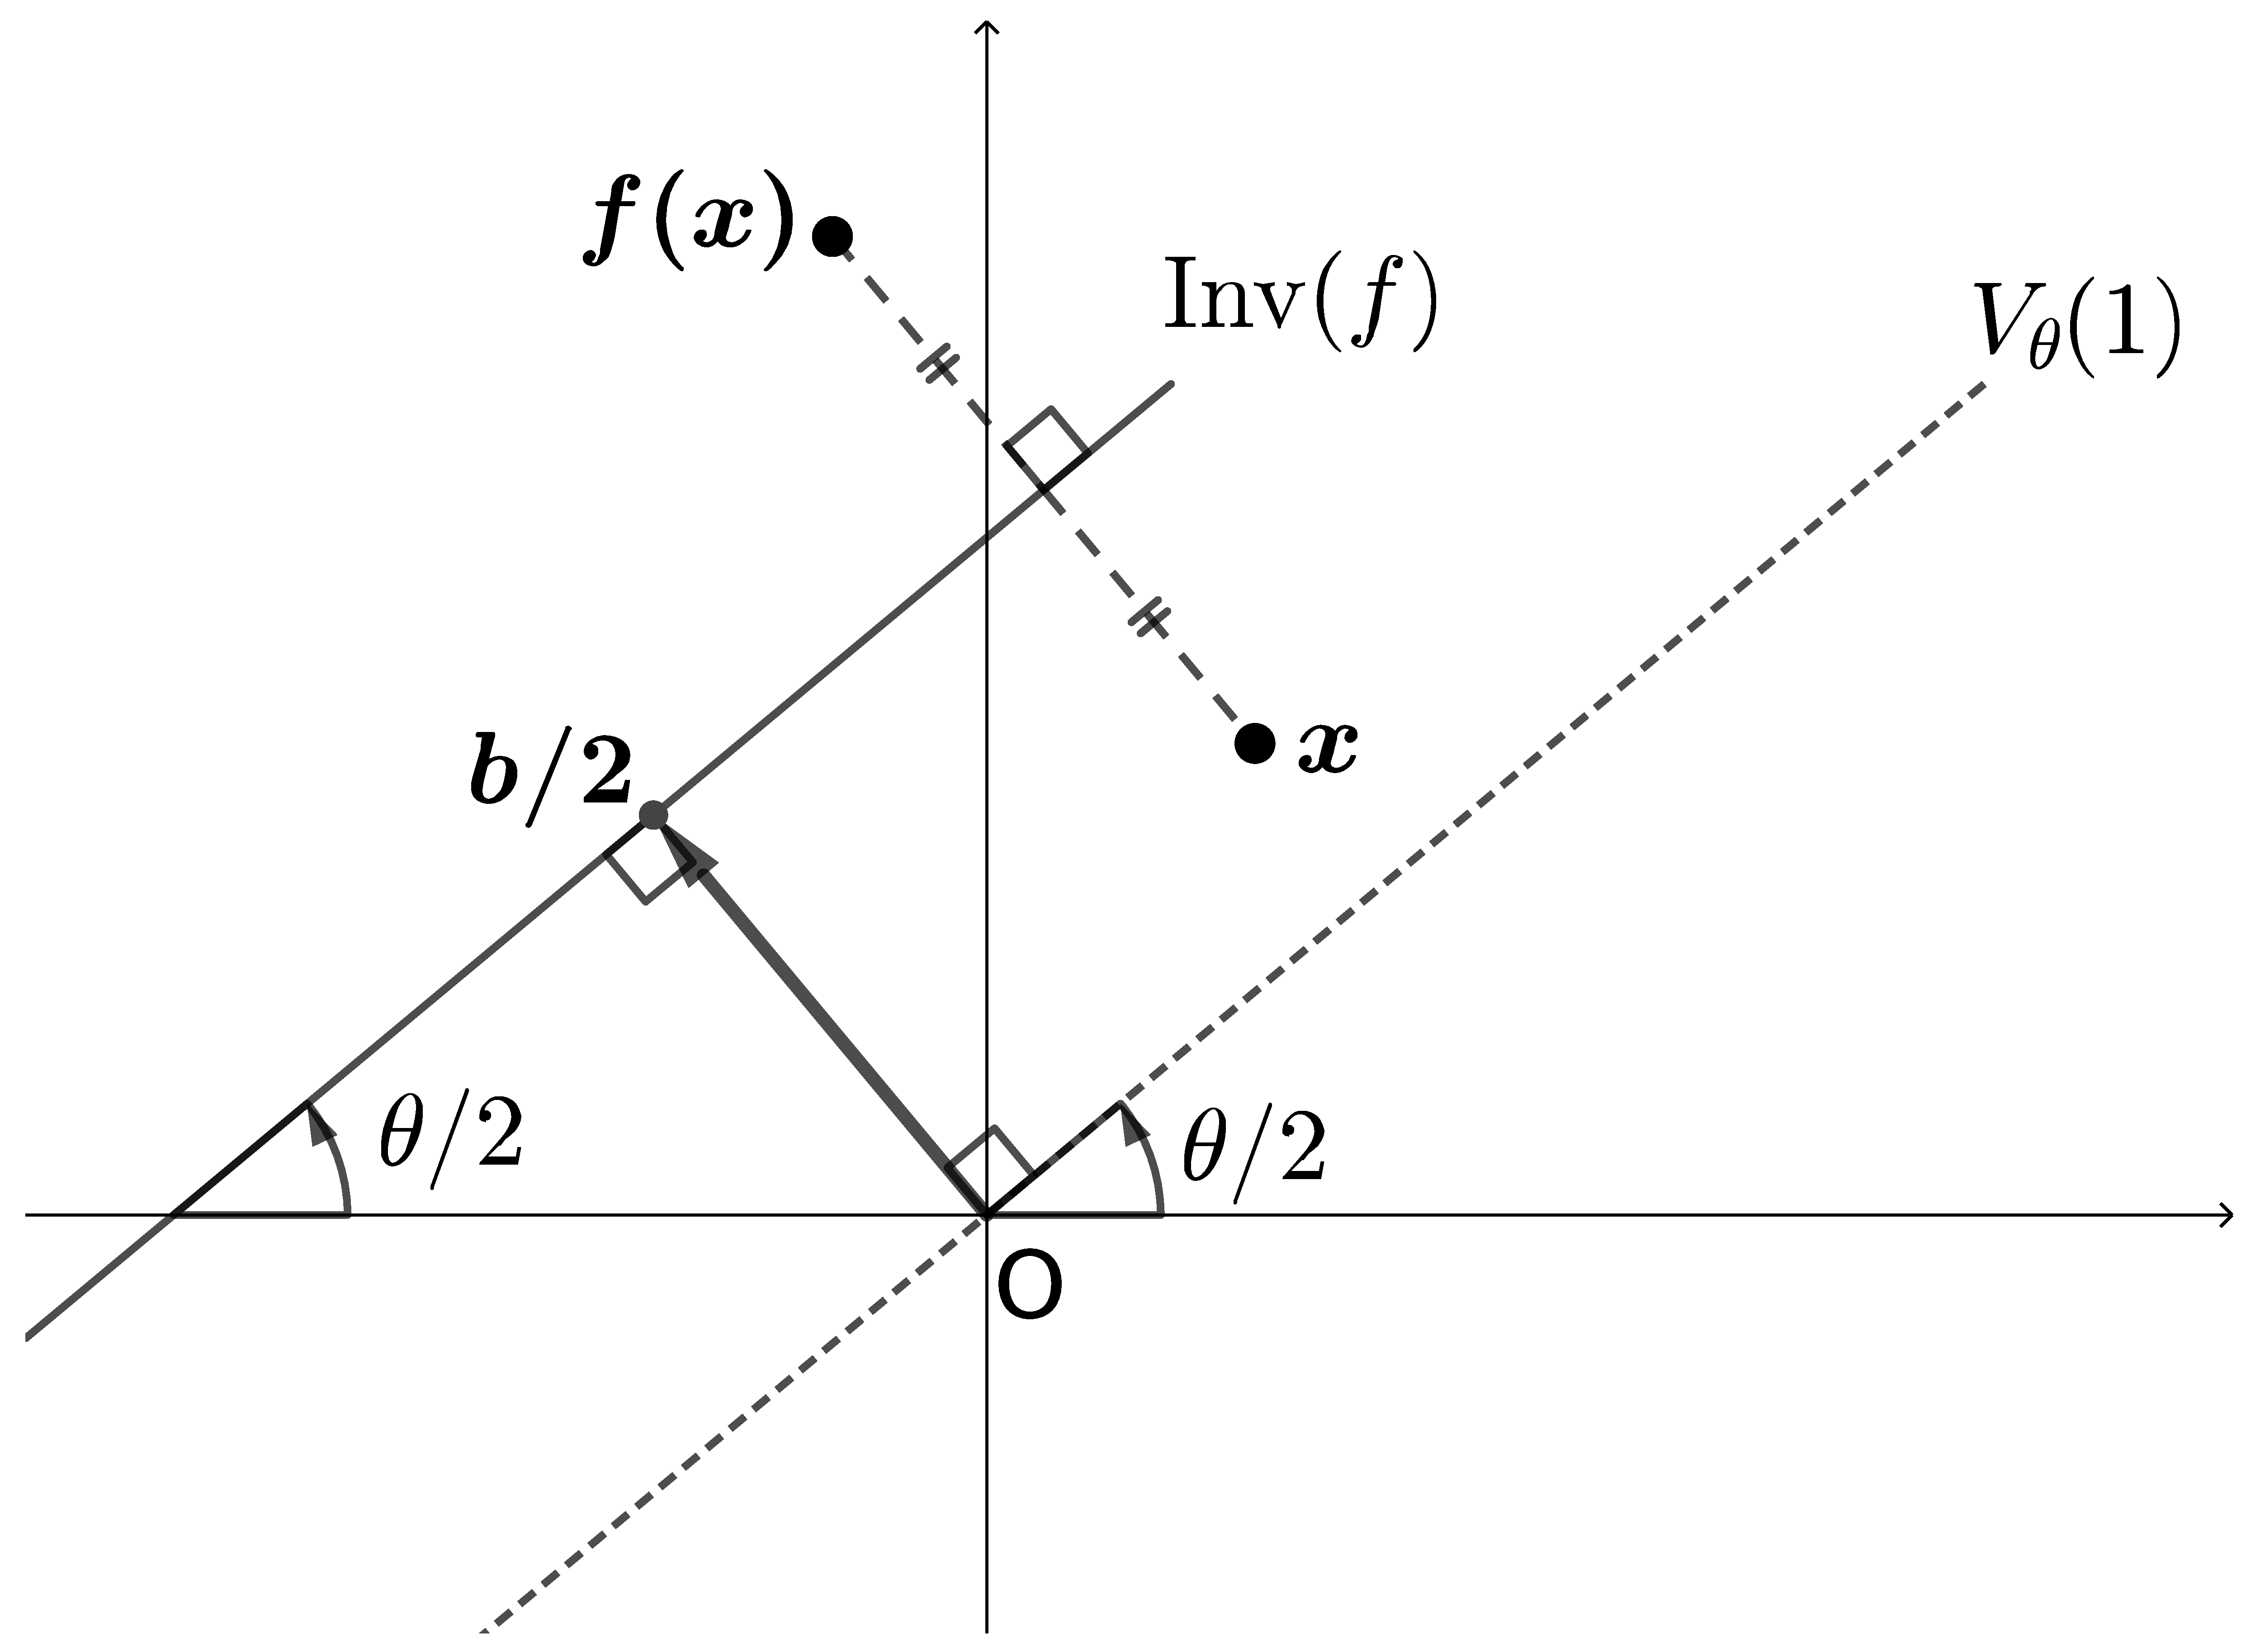
\includegraphics[height=5cm]{pictures/reflection2gen.pdf}
  \caption{直線 $\Fix(f)$ に関する鏡映}
  \label{fig:reflection2gen}
\end{figure}

なお,任意の $\bm{c} \in \Fix(f)$ に対して
\[
  f(\bm{x}) =  R_{\theta}\left( \bm{x} - \bm{c}\right) + \bm{c}
\]
が成り立つから,
\[
  f = t_{\bm{c}} \circ r_{\theta} \circ t_{-\bm{c}}
\]
である.すなわち,$\bm{c}$ を通り $V_{R_{\theta}}(1)$ に平行な直線に関する
鏡映は「一旦 $-\bm{c}$ 平行移動し,$V_{R_{\theta}}(1)$ に関する鏡映移動をし
た後に再び $\bm{c}$ 平行移動する変換」と言い換えることもできる(
図\ref{fig:reflection2gen2}).
\begin{figure}[h]
  \centering
  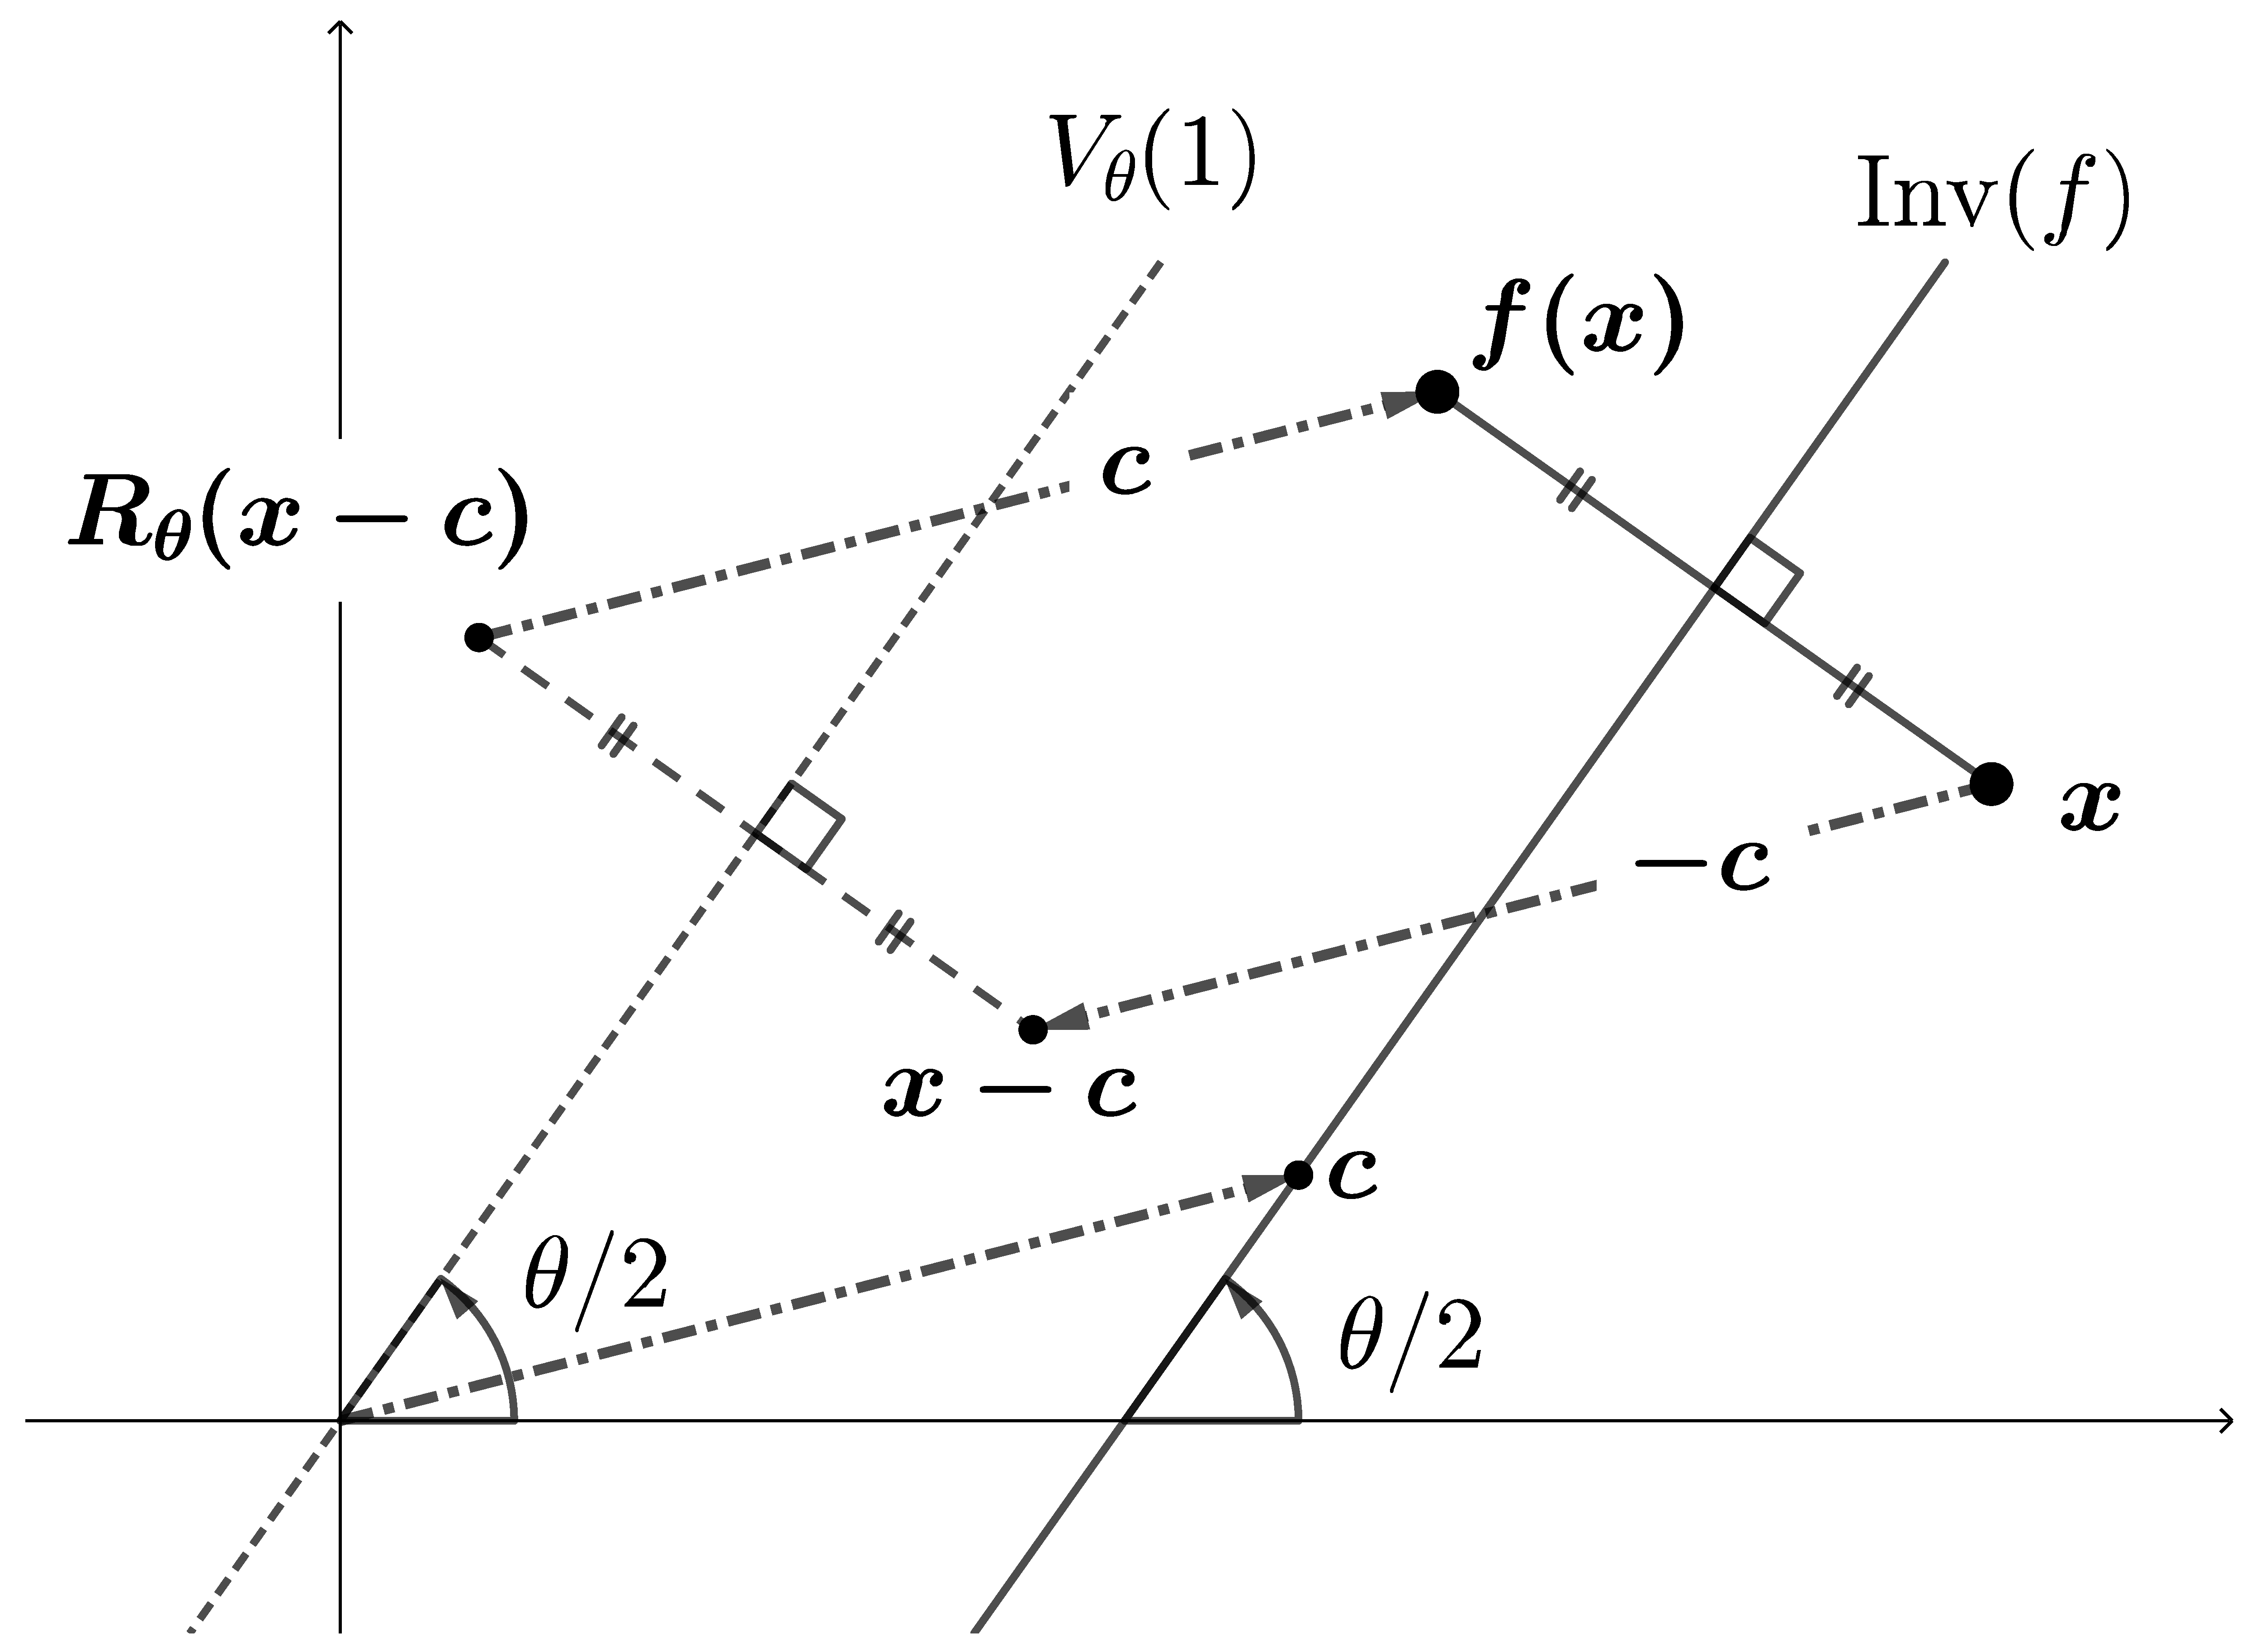
\includegraphics[height=5cm]{pictures/reflection2gen2.pdf}
  \caption{$\bm{c}$ を通り $V_{R_{\theta}}(1)$ に平行な直線に関する鏡映}
  \label{fig:reflection2gen2}
\end{figure}


続いて,$\bm{b} \notin V_{R_{\theta}}(-1)$ とする.このとき $f$ は滑り鏡映で
あることを確かめよう.なお,平面上の滑り鏡映の定義は次の通りである.

\begin{definition}
  平面上の直線 $L$ に関する鏡映 $g$ と $L$ に平行なベクトル $\bm{c}
  \in \mathbb{R}^2$ による平行移動 $t_{\bm{c}}$ との合成 $t_{\bm{c}}
  \circ g$ を $L$ と $\bm{c}$ に関する滑り鏡映または並進鏡
  映という.この定義に従えば滑り鏡映は鏡映($\bm{c}=\bm{0}$ のとき)
  を含むのだが,本稿では鏡映でないもののみを滑り鏡映と呼ぶことにする.
\end{definition}


今 $\bm{b} \notin V_{R_{\theta}}(-1)$ としているので,$\bm{b}$ を式 (\ref{eq:eigendecomp2})のように分解する
と $\bm{b}^{+} \neq \bm{0}$ である.従って,
\[
  f(\bm{x}) = \left(R_{\theta}\bm{x} + \bm{b}^{-}\right) + \bm{b}^{+}
\]
である.$g(\bm{x}) = R_{\theta}\bm{x}+\bm{b}^{-}$
とおくと,$f= t_{\bm{b}^{+}} \circ g$ である.$\bm{b}^{-} \in
V_{R_{\theta}}(-1)$ だから $g$ は直線 $\Fix(g)$ に関する鏡映である.ま
た,$\bm{b}^{+} \in V_{R_{\theta}}(1)$ より $\bm{b}^{+}$ は $\Fix(g)$ と平
行である.よって,$f$ は $\bm{b}^{-}/2$ を通り $V_A(1)$ に平行な直線と
ベクトル $\bm{b}^{+}$ に関する滑り鏡映である(図\ref{fig:glide2}).
 \begin{figure}[h]
   \centering
   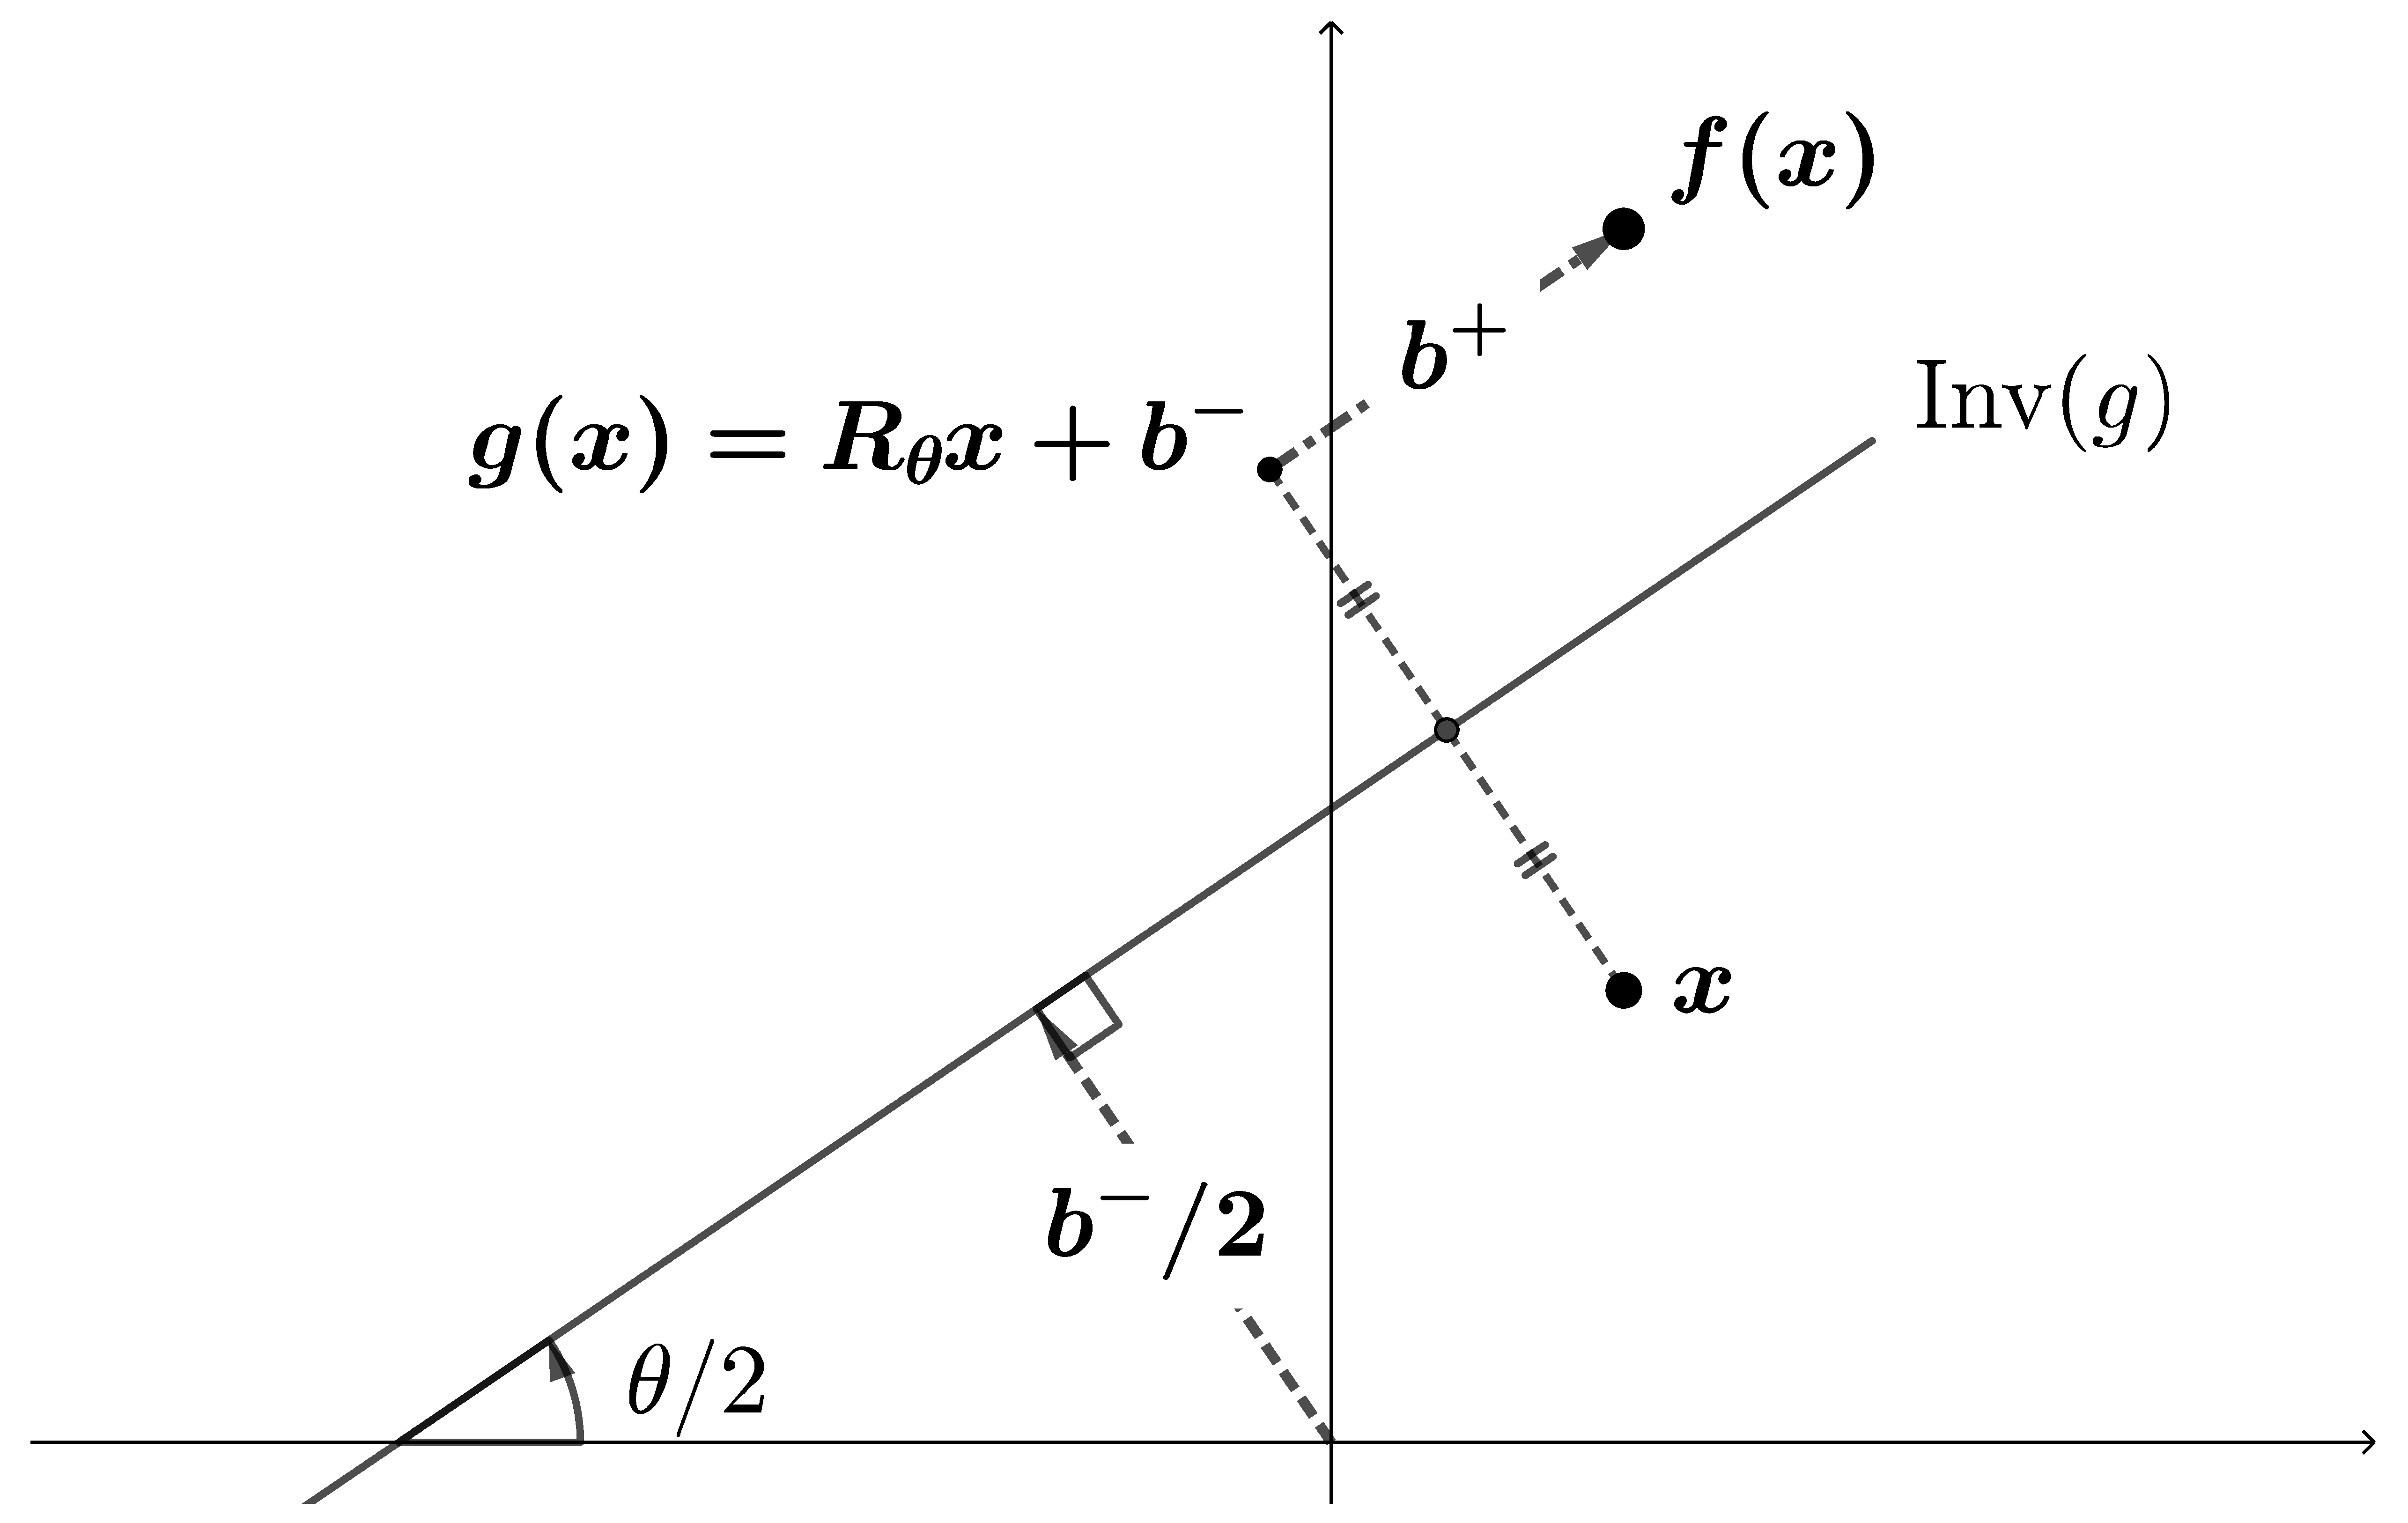
\includegraphics[height=5cm]{pictures/glide2.pdf}
   \caption{滑り鏡映}
   \label{fig:glide2}
 \end{figure}

 なお,鏡映と平行移動を合成する順番はどちらでもよい.実際,$R_{\theta}\bm{b}^{+}=\bm{b}^{+}$ より
\[
  g \left(t_{\bm{b}^{+}}(\bm{x})\right) = R_{\theta}\left(\bm{x} + \bm{b}^{+}\right) + \bm{b}^{-}
  = \left(R_{\theta}\bm{x} + \bm{b}^{-}\right) + \bm{b}^{+} = t_{\bm{b}^{+}}\left(g(\bm{x})\right)
\]
であるから,$g \circ t_{\bm{b}^{+}} = t_{\bm{b}^{+}} \circ g$ である.

 最後に,内積による鏡映と滑り鏡映の判別方法をまとめておこ
 う.$R_{\theta}$ の単位固有ベクトルに
 \[
   \bm{p}^{+}_{\theta} = \left[
     \begin{array}{r}
       \cos(\theta/2)\\
       \sin(\theta/2)
     \end{array}
   \right] \in V_{R_{\theta}}(1), \quad \bm{p}^{-}_{\theta} = \left[
     \begin{array}{r}
       -\sin(\theta/2)\\
       \cos(\theta/2)
     \end{array}
   \right] \in V_{R_{\theta}}(-1)
 \]
 と名前を付ける.$\left(\bm{p}_{\theta}^{+}, \bm{p}_{\theta}^{-}\right)$ は $\mathbb{R}^2$ の
 正規直交基底だから式(\ref{eq:eigendecomp2})における $\bm{b}^{+},
 \bm{b}^{-}$ はそれぞれ
 \[
   \bm{b}^{+} = (\bm{b}, \bm{p}_{\theta}^{+}) \bm{p}_{\theta}^{+} ,
   \quad  \bm{b}^{-} =  (\bm{b}, \bm{p}_{\theta}^{-})\bm{p}_{\theta}^{-}
 \]
 と表せる.これより,合同変換 $f(\bm{x}) = R_{\theta} \bm{x} + \bm{b}$
 は以下の2つに分けられる.
 \begin{itemize}
   \setlength{\itemsep}{1zh}
 \item $\bm{b} \cdot \bm{p}_{\theta}^{+}=0$ のと
   き,$f$ は $\bm{b}/2$ を通り $V_{R_{\theta}}(1)$ に平行な直線に関する鏡
   映である.
   
 \item $\bm{b} \cdot  \bm{p}_{\theta}^{+} \neq 0$ のと
   き,$f$ は
   $\left(\bm{b} \cdot \bm{p}_{\theta}^{-}\right)\bm{p}_{\theta}^{-}/2$ を通
   り $V_{R_{\theta}}(1)$ に平行な直線とベクト
   ル $(\bm{b}\cdot \bm{p}_{\theta}^{+})\bm{p}_{\theta}^{+}$ に関する滑り鏡
   映である.
 \end{itemize}



\subsection{鏡映の個数}

平面の合同変換それぞれに対し,それを合成する鏡映を全て調べ上げ,分
類表\ref{tab:classification2}を完成させよう.

% \begin{definition}
%   平面上の $3$ 点が同一直線上にないとき,その $3$ 点は一般の位置にある
%   という.
% \end{definition}

% \begin{theorem}\label{thm:identity2}
%   平面上の一般の位置にある $3$ 点を固定する合同変換は恒等変換である.
% \end{theorem}

% \begin{proof}
%   $\bm{p}_0, \bm{p}_1, \bm{p}_2 \in \mathbb{R}^2$ は一般の位置にあると
%   し,平面の合同変換 $f$ は $\bm{p}_0, \bm{p}_1, \bm{p}_2$ を固定すると
%   する.このとき,$\bm{p}_0, \bm{p}_1, \bm{p}_2 \in \Fix(f)$ だか
%   ら $\Fix(f)$ 空でも $1$ 点集合でもない.さらに,$\bm{p}_0, \bm{p}_1,
%   \bm{p}_2$ は同一直線上にないから $\Fix(f)$ は直線でもない.よっ
%   て,\ref{sec:inv2}節で見たように $\Fix(f)=\mathbb{R}^2$ であるか
%   ら $f$ は恒等変換である.
% \end{proof}





\begin{theorem}\label{thm:generate2}
  平面 $\mathbb{R}^2$ の任意の合同変換は
  $3$個以下の鏡映の合成として表せる.特に,各合同変換に対してそれを合成
  する鏡映の最小個数は表\ref{tab:classification2}にある通りである.
\end{theorem}
\begin{proof}
  恒等変換は $0$ 個,鏡映は $1$ 個の鏡映の合成であり,またそれ以外の合
  同変換は $1$ 個以下の鏡映の合成として表せないは明らかである.残りの平
  行移動,回転,滑り鏡映に関しては以下に続く補
  題\ref{lem:translation2ref},補題\ref{lem:rotaion2ref},補
  題\ref{lem:glide2ref}により証明が完成する.
\end{proof}

  
\begin{lemma}\label{lem:translation2ref}
  \begin{enumerate}[(1)]
  \item 平面 $\mathbb{R}^2$ の平行移動 $t_{\bm{b}} \; (\bm{b} \neq
    \bm{0})$ は平行な $2$ 直線に関する $2$ 個の鏡映の合成である.このと
    き,$2$ つの鏡映軸は共に $\bm{b}$ に直交し,その距離
    は $\|\bm{b}\|/2$ である.
    
  \item 逆に,平面 $\mathbb{R}^2$ の平行な $2$ 直線 $L_1, L_2 \;(L_1
    \neq L_2)$ に関する鏡映 $g_1, g_2$ の合成 $g_2 \circ g_1$ は平行移
    動である.移動方向は $L_1$ から $L_2$ の方へ両直線に直交する方向で,
    移動距離は $2$ 直線の距離の $2$ 倍である.
  \end{enumerate}
  
\end{lemma}

\begin{proof}
  (1) $\bm{b} \in V_{R_{\theta}}(-1)$ となる $\theta \in \mathbb{R}$ をとる.
  このとき,合同変換 $g(\bm{x})=R_{\theta}\bm{x}+\bm{b}$ は $\bm{b}/2$
  を通り $V_{R_{\theta}}(1)$ を通る直線 $L$ に関する鏡映である.従って,任
  意の $\bm{x} \in \mathbb{R}^2$ に対して
  \[
    g\left(r_{\theta}(\bm{x})\right) =
    R_{\theta}\left(R_{\theta}\bm{x}\right)+\bm{b} =
    \bm{x}+\bm{b}=t_{\bm{b}}(\bm{x})
  \]
  であるから $t_{\bm{b}}$ は $2$ 個の鏡映の合成 $g \circ r_{\theta}$ で
  ある.また,図\ref{fig:translation2}のように $g, r_{\theta}$ の鏡映
  軸 $L, V_{R_{\theta}}(1)$ はそれぞれ $\bm{b}/2, \bm{0}$ を通り共
  に $\bm{b}$ に直交し,$2$ 直線の距離は $\|\bm{b}\|/2$ である.
  \begin{figure}[h]
    \centering
    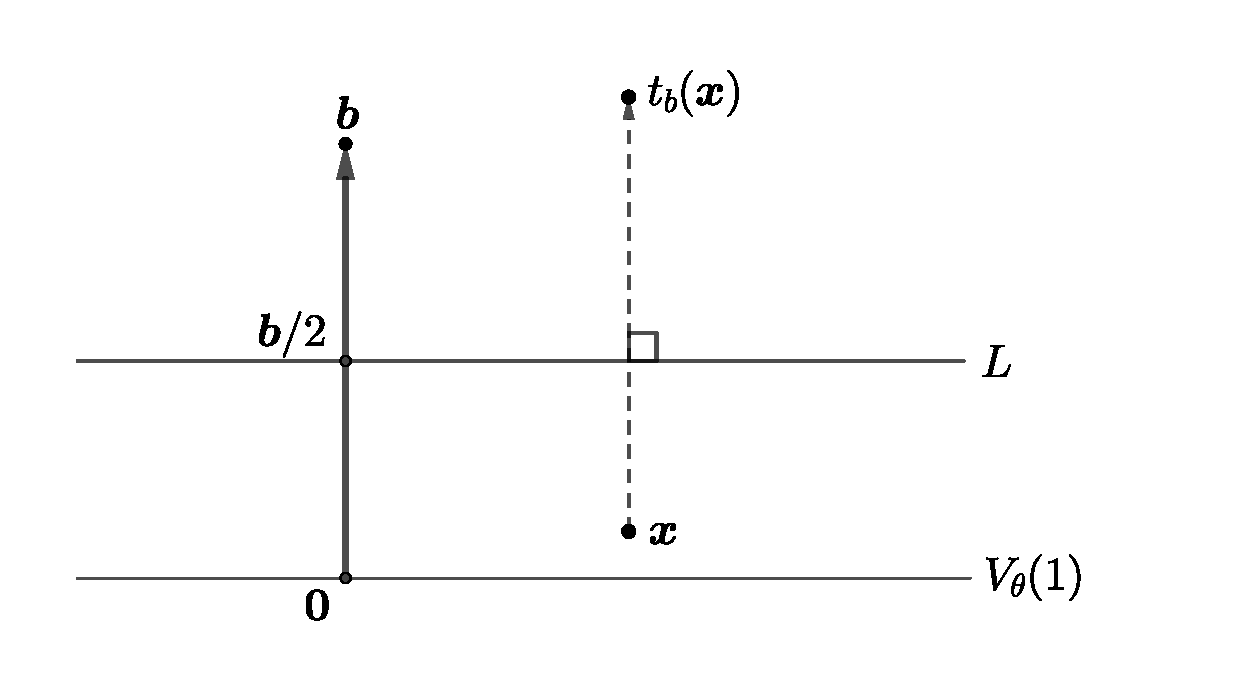
\includegraphics[height=5cm]{pictures/translation2.pdf}
    \caption{平行移動は平行な $2$ 直線に関する鏡映の合成である.}
    \label{fig:translation2}
  \end{figure}

  \noindent
  (2) 逆に,平行な $2$ 直線 $L_1, L_2 \; (L_1 \neq L_2)$ に関する鏡映の
  合成が平行移動となることを示す.$L_1, L_2$ が $x$ 軸とのなす角
  を $\theta/2$ とすると,$L_1, L_2$ に関する鏡映 $g_1, g_2$ は
  \[
    g_1(\bm{x}) = R_{\theta} \bm{x} + \bm{b}_1, \quad  g_2(\bm{x}) =R_{\theta}\bm{x} + \bm{b}_2 
    \quad \left( \bm{b}_1, \bm{b}_2 \in V_{R_{\theta}}(-1), \; \bm{b}_1 \neq \bm{b}_2\right)
  \]
  と書ける.ただし,$L_1, L_2$ はそれぞれ $\bm{b}_1/2, \bm{b}_2/2$ を通
  る.これより任意の $\bm{x} \in \mathbb{R}^2$ に対して
  \[
    g_2 \circ g_1 (\bm{x}) = R_{\theta}\left(R_{\theta}\bm{x} + \bm{b}_1\right)+\bm{b}_2
    = \bm{x} + \bm{b}_2 - \bm{b}_1
  \]
  だから,$g_2 \circ g_1$ は平行移動 $t_{\bm{b}_2-\bm{b}_1}$ である.ま
  た,図\ref{fig:translation2gen}のようにその移動方向
  は $L_1$ から $L_2$ の方へ両直線に直交する方向であり,移動距
  離 $\|\bm{b}_2-\bm{b}_1\|$ は $L_1, L_2$ の距離の $2$ 倍である.
  \begin{figure}[h]
    \centering
    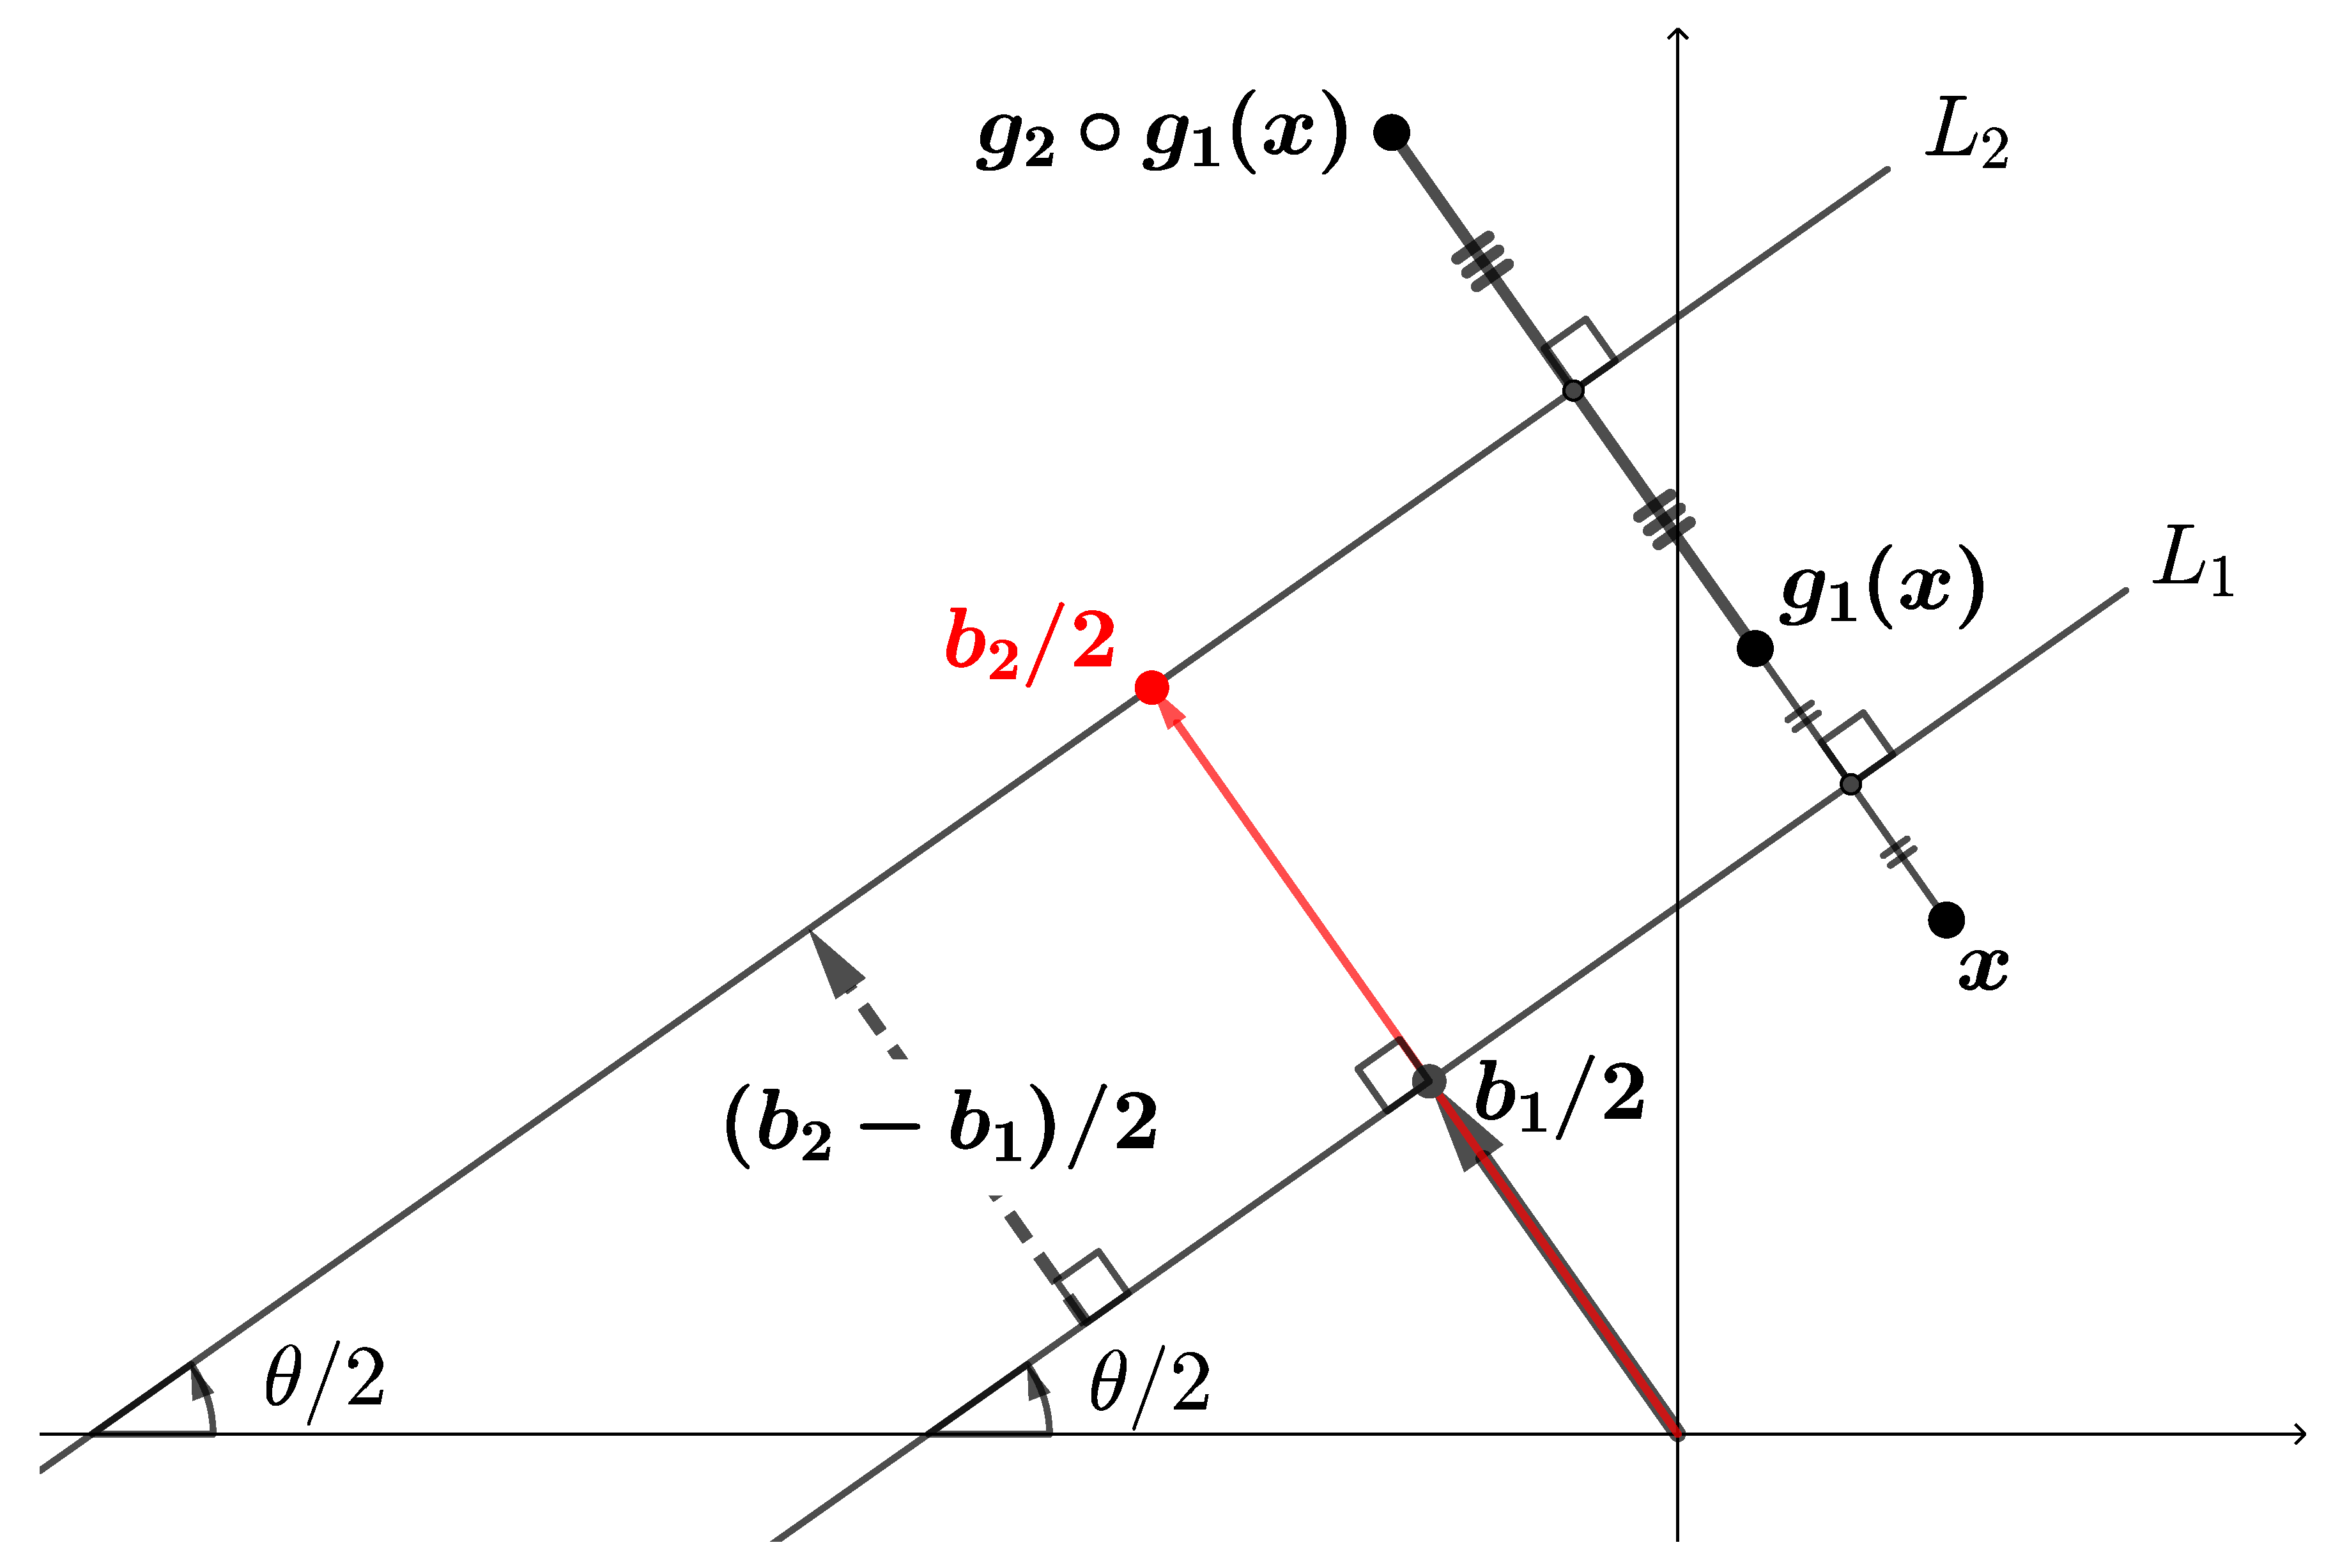
\includegraphics[height=5cm]{pictures/translation2gen.pdf}
    \caption{鏡映軸が平行な2つの鏡映の合成は平行移動である.}
    \label{fig:translation2gen}
  \end{figure}
\end{proof}

\begin{lemma}\label{lem:rotaion2ref}
  \begin{enumerate}[(1)]
  \item 平面 $\mathbb{R}^2$ の $\theta$ 回転は回転の中心で交わる $2$ 直
    線に関する $2$ 個の鏡映の合成である.このとき,鏡映軸同士のなす角
    は $\theta/2$ である.

  \item 逆に,平面 $\mathbb{R}^2$ の平行でない $2$ 直線 $L_1, L_2$ に関
    する鏡映 $g_1, g_2$ の合成 $g_2 \circ g_1$ は $2$ 直線の交点を中心
    とする $L_1$ から $L_2$ の方への回転である.回転角は $2$ 直線
    のなす角の $2$ 倍である.
  \end{enumerate}
\end{lemma}

\begin{proof}
  (1) $f$ を $\bm{c} \in \mathbb{R}^2$ を中心とする平面の $\theta$ 回転
  とする.$f(\bm{x}) = S_{\theta}(\bm{x}-\bm{c})+\bm{c}$ と書ける.
  \[
    g_1(\bm{x})=R_0(\bm{x}-\bm{c})+\bm{c}, \quad g_2 (\bm{x}) = R_{\theta}(\bm{x}-\bm{c})+\bm{c}
    \quad (\theta \neq 0)
  \]
  とすると,$g_1$ は $x$ 軸に平行で $\bm{c}$ を通る直線 $L_1$ に関する
  鏡映であり,$g_2$ は $V_{R_{\theta}}(1)$に平行で $\bm{c}$ を通る直
  線 $L_2$ に関する鏡映である.このとき,任意の $\bm{x} \in
  \mathbb{R}^2$ に対して
  \begin{align*}
    g_2 \circ g_1(\bm{x}) = R_{\theta}\left( R_{0}(\bm{x}-\bm{c}) + \bm{c} - \bm{c} \right) + \bm{c}
    = S_{\theta} (\bm{x}-\bm{c}) +\bm{c} = f(\bm{x})
  \end{align*}
  より,$f$ は $2$ 個の鏡映の合成 $g_2 \circ g_1$ である.
  図\ref{fig:rotation2ref}のように鏡映軸 $L_1, L_2$ のなす角
  は $\theta/2$ である.
  \begin{figure}[h]
    \centering
    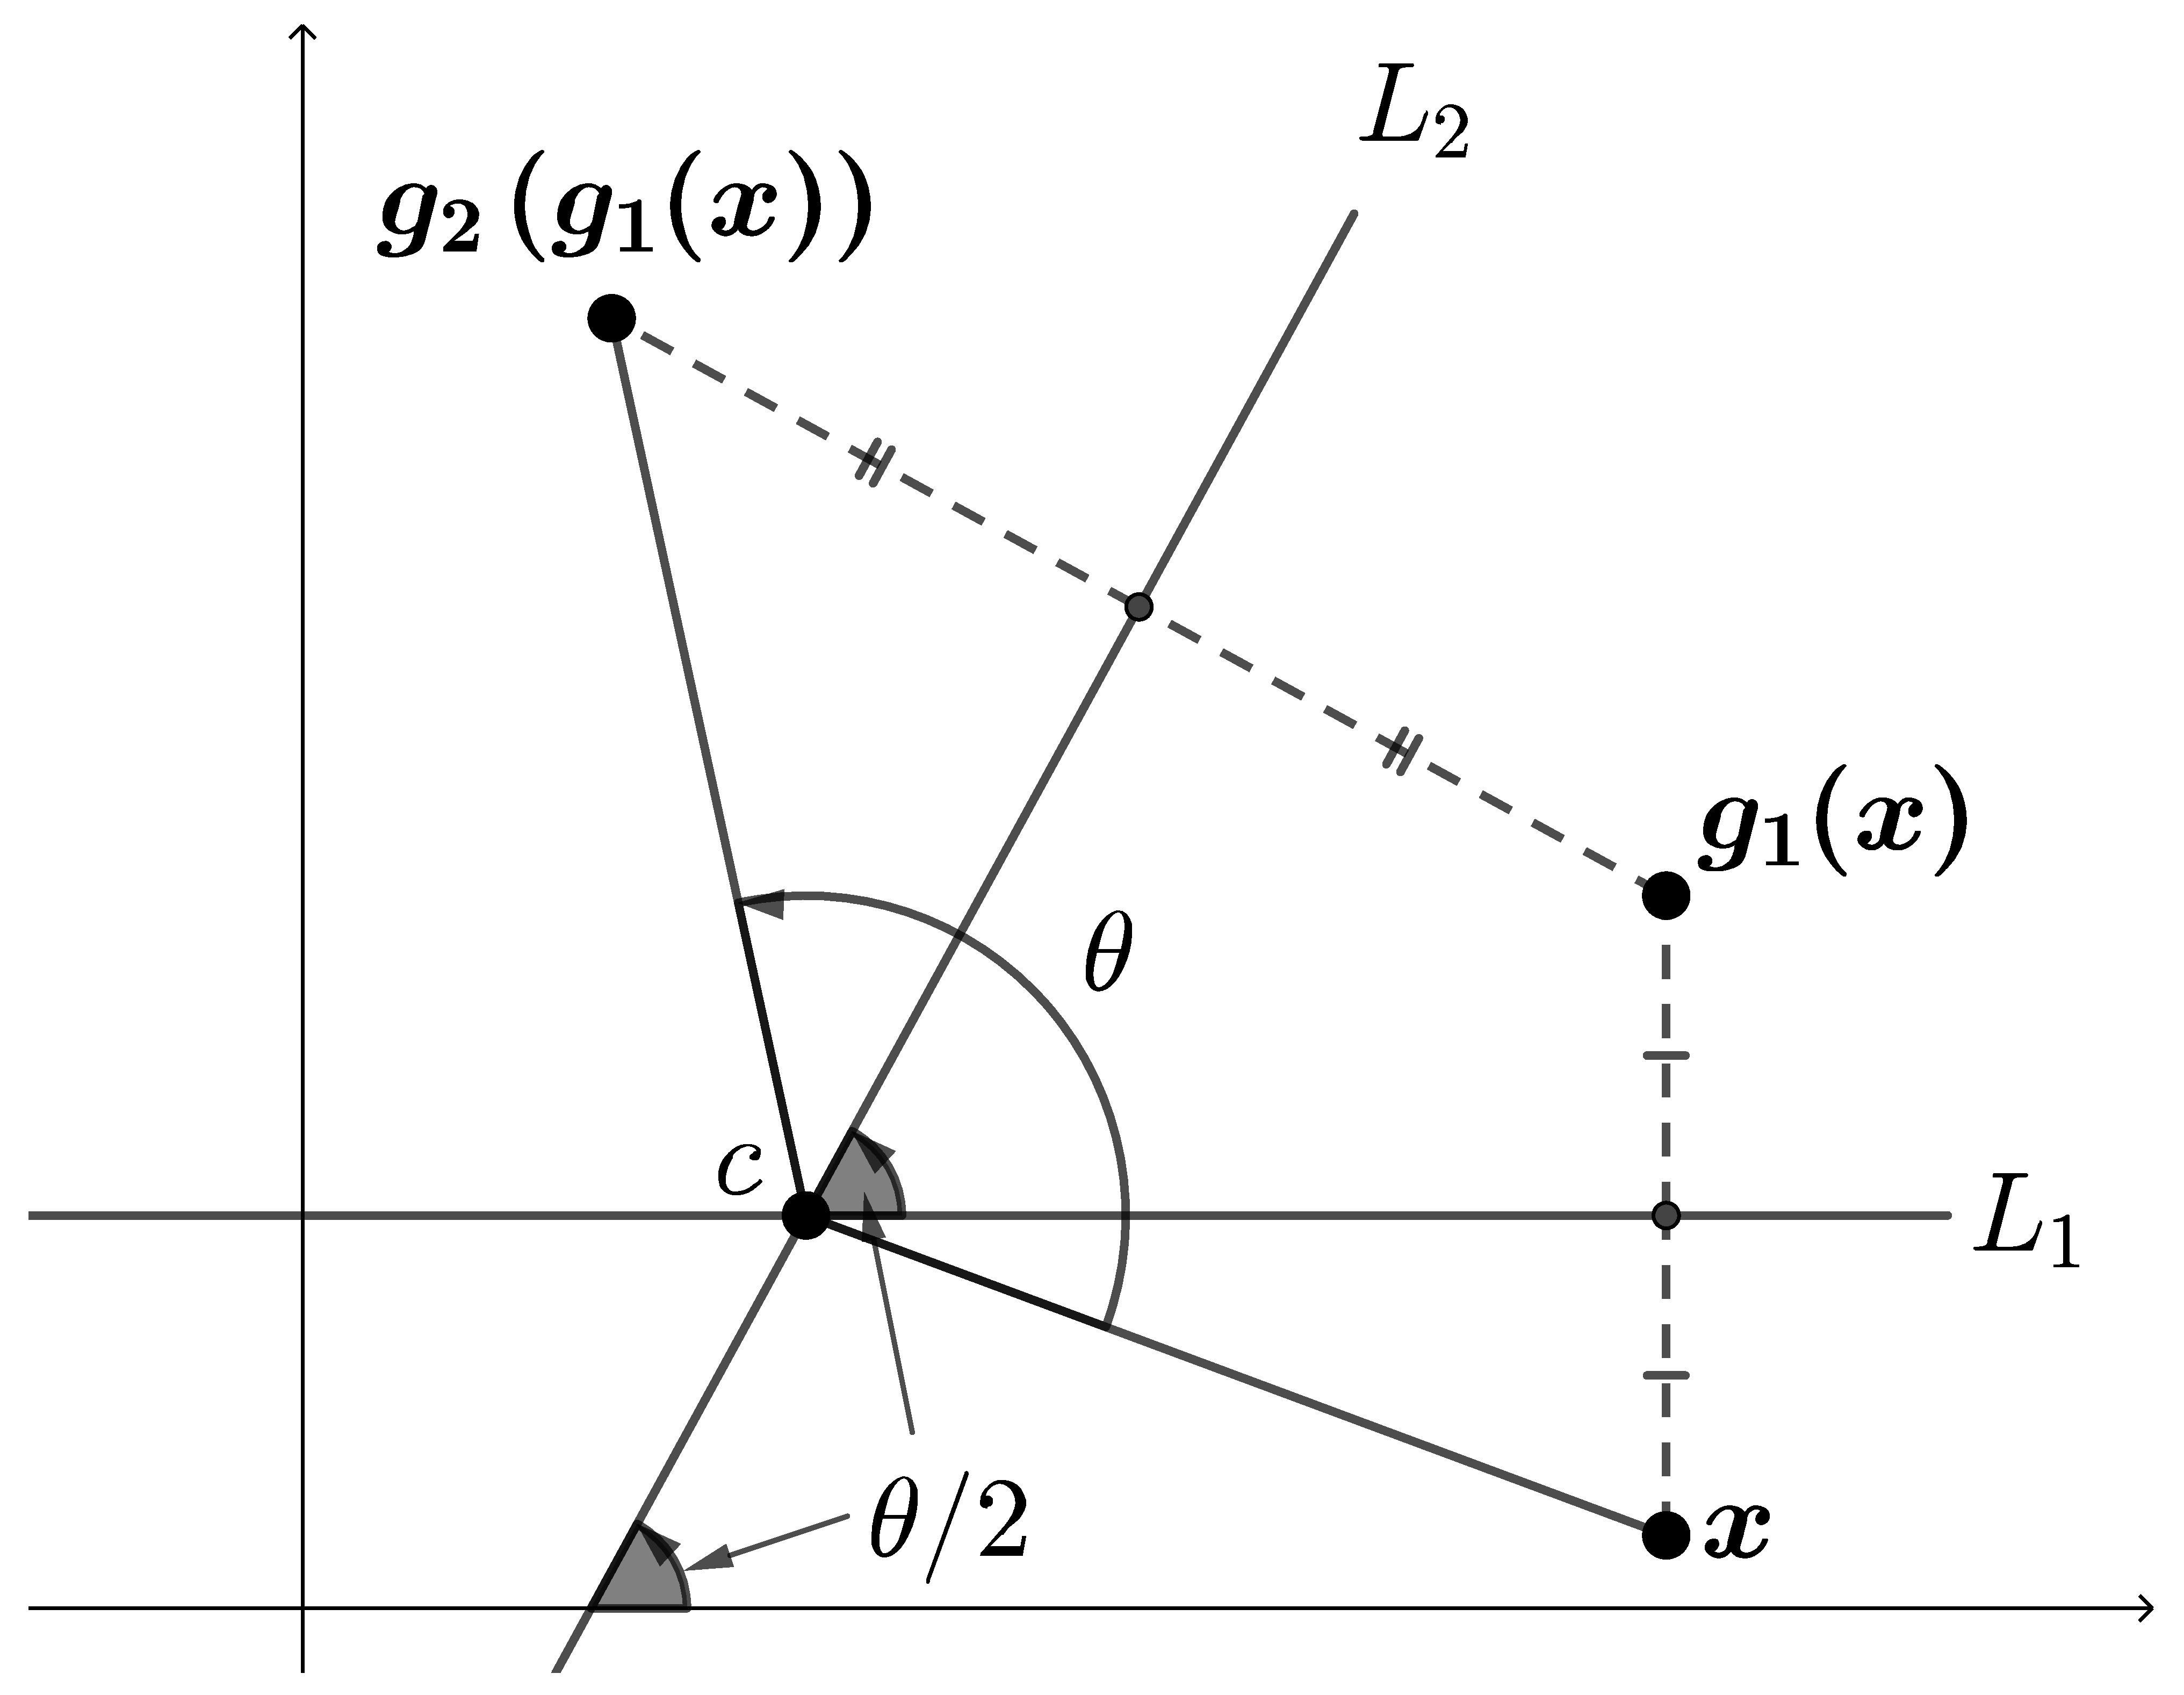
\includegraphics[height=5cm]{pictures/rotation2ref.pdf}
    \caption{回転は平行でない $2$ 直線に関する鏡映の合成である.}\label{fig:rotation2ref}
  \end{figure}

  \noindent
  (2) 逆に,平行でない $2$ 直線 $L_1, L_2$ に関する鏡映の合成が回転とな
  ることを示す.$L_1, L_2$ が $x$ 軸となす角をそれぞれ $\theta/2,
  \phi/2$ とすると,$L_1, L_2$ に関する鏡映 $g_1, g_2$ は
  \[
    g_1(\bm{x}) = R_{\theta} \bm{x} + \bm{b}_1, \quad g_2(\bm{x}) = R_{\phi}\bm{x} + \bm{b}_2 \quad
    \left(\bm{b}_1 \in V_{R_{\theta}}(-1), \; \bm{b}_2 \in V_{\phi}(-1) \right)
  \]
  と書ける.ただし,$L_1, L_2$ はそれぞれ $\bm{b}_1/2, \bm{b}_2/2$ を通
  る.これより任意の $\bm{x} \in \mathbb{R}^2$ に対して
  \[
    g_2 \circ g_1(\bm{x}) = R_{\phi}( R_{\theta}\bm{x}+\bm{b}_1) + \bm{b}_2
    = S_{\phi-\theta} \bm{x} + R_{\phi}\bm{b}_1 +\bm{b}_2
  \]
  だから,$g_2 \circ
  g_1$ は
  $\bm{c}:=(E-S_{\phi-\theta})^{-1}\left(R_{\phi}\bm{b}_1+\bm{b}_2\right)$
  を中心とする $\phi-\theta$ 回転である.鏡映軸 $L_1, L_2$ の交点
  を $\bm{c}' \in L_1 \cap L_2$ とすると,$\bm{c}' \in \Fix(g_2 \circ
  g_1)$ である.回転の固定点は中心点だけなので $\bm{c}'=\bm{c}$ である.
  また,図\ref{fig:rotation2refgen}のように回転方向は $L_1$ から $L_2$
  の方へ,回転角 $\phi-\theta$ は $L_1$ と $L_2$ のなす角の $2$ 倍である.
  \begin{figure}[h]
    \centering
    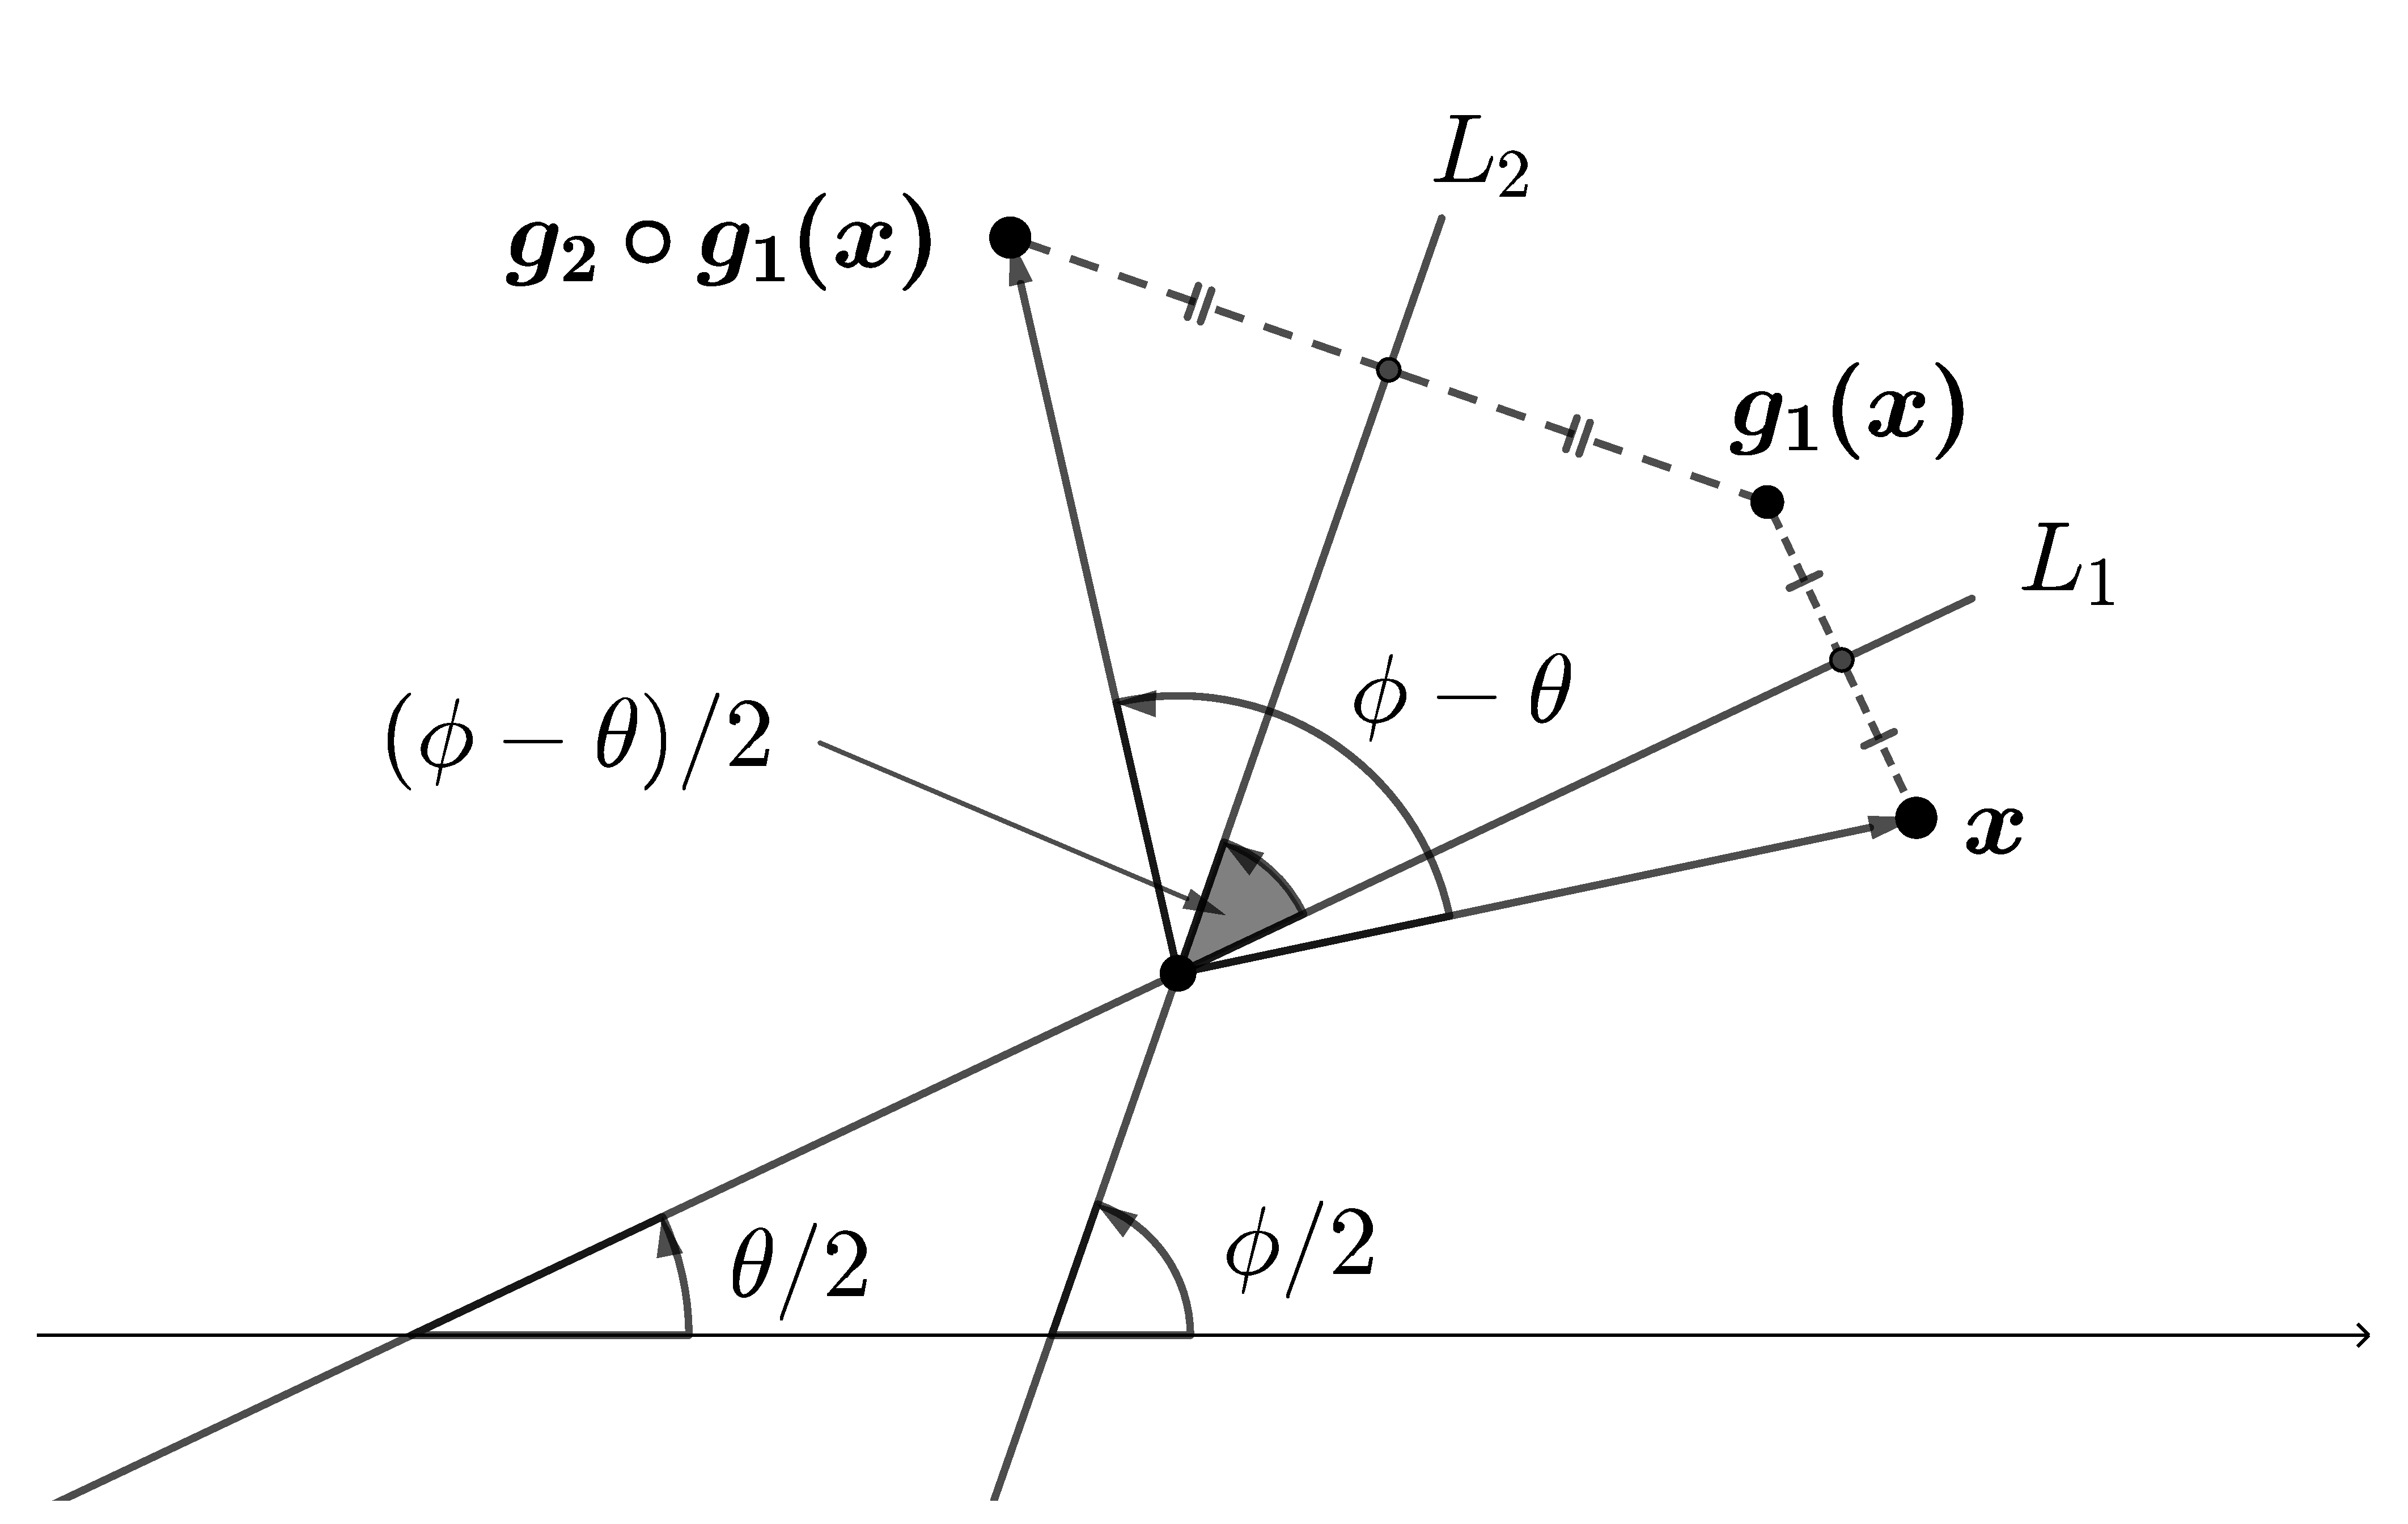
\includegraphics[height=5cm]{pictures/rotation2refgen.pdf}   
    \caption{鏡映軸が平行でない2つの鏡映の合成は回転である.}
    \label{fig:rotation2refgen}
  \end{figure}
\end{proof}


\begin{lemma}\label{lem:glide2ref}
  平面 $\mathbb{R}^2$ の滑り鏡映は $3$ 個の鏡映の合成として表せる.また,
  滑り鏡映は $2$ 個以下の鏡映の合成としては表せない.
\end{lemma}
  
\begin{proof}
  $f$ を平面 $\mathbb{R}^2$
  の滑り鏡映とする.$f(\bm{x}) = R_{\theta}\bm{x} + \bm{b} \; (\theta
  \neq 0, \; \bm{b} \notin V_{R_{\theta}}(-1))$ と書ける.
  \[
    \bm{b} = \bm{b}^{+} + \bm{b}^{-}, \quad \bm{b}^{+} \in
    V_{R_{\theta}}(1), \quad \bm{b}^{-} \in V_{R_{\theta}}(-1),
    \quad \bm{b}^{+} \neq \bm{0}
  \]
  とし,$g_1(\bm{x}) = R_{\theta} \bm{x} + \bm{b}^{-}$ とす
  る.$g_1$ は $\bm{b}^{-}/2$ を通り $V_{R_{\theta}}(1)$ に平行な直
  線 $L_1$ に関する鏡映である.
  \[
    f(\bm{x}) = \left( R_{\theta}\bm{x} + \bm{b}^{-}\right) +
    \bm{b}^{+} = t_{\bm{b}^{+}}\left( g_1(\bm{x})\right)
  \]
  より,$f=t_{\bm{b}^{+}}\circ g_1$ である.さらに,補
  題\ref{lem:translation2ref}(1)より平行移
  動 $t_{\bm{b}^{+}}$ は図\ref{fig:glide2ref}のように平行
  な $2$ 直線 $L_2, L_3$ に関する鏡映 $g_2, g_3$ の合成として表せる.実
  際,$L_2, L_3$ をそれぞれ $\bm{0}, \bm{b}^{+}/2$ を通り共
  に $\bm{b}^{+}$ に垂直な直線とすれば $t_{\bm{b}^{+}} = g_2 \circ
  g_1$ である.よって,
  \[
    f = g_3 \circ g_2 \circ g_1
  \]
  より $f$ は $3$ 個の鏡映の合成である.また,補
  題\ref{lem:translation2ref}(2)と補題\ref{lem:rotaion2ref}(2)から $2$
  個の鏡映の合成は恒等変換か平行移動か回転なので,滑り鏡映を $2$ 個以下
  の鏡映の合成として表すことはできない.
  \begin{figure}[h]
    \centering
    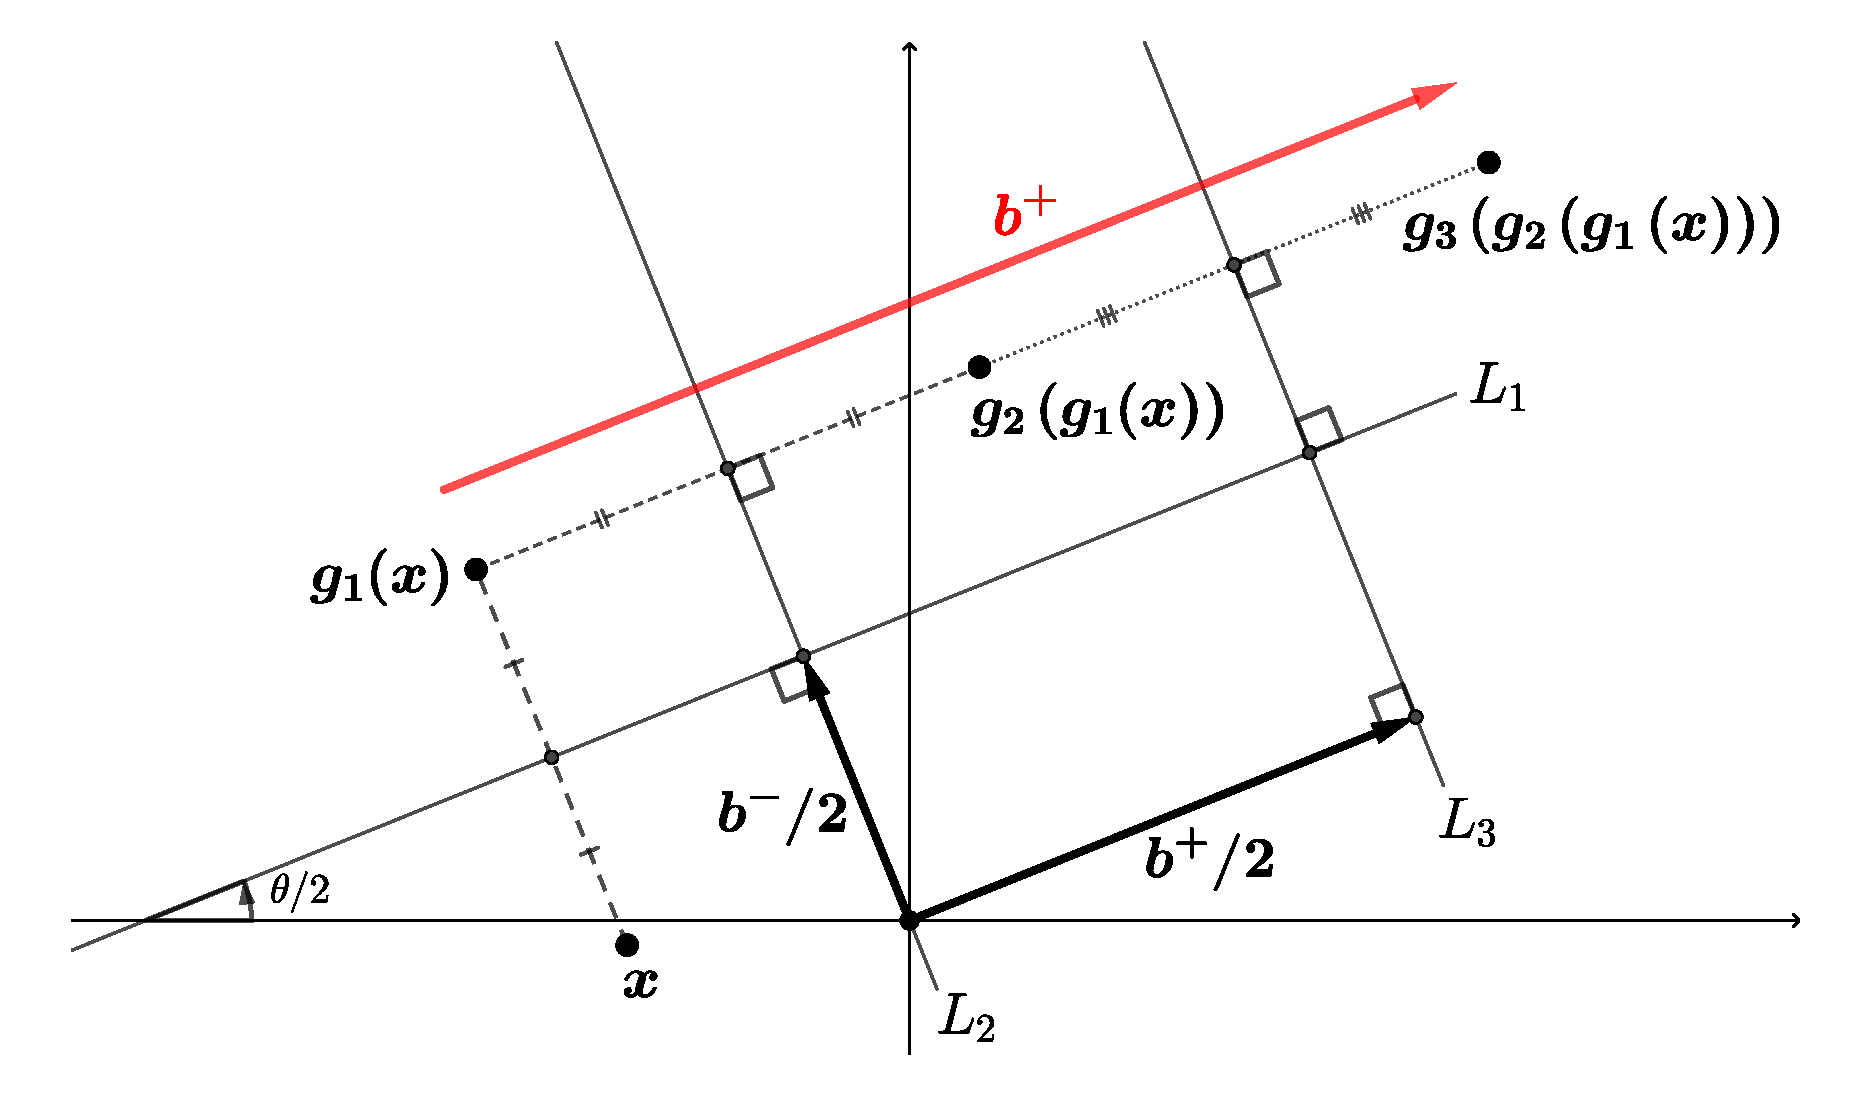
\includegraphics[height=5cm]{pictures/glide2ref.pdf}
    \caption{滑り鏡映は $3$ 個の鏡映の合成である.}
    \label{fig:glide2ref}
  \end{figure}
\end{proof}



\subsection{平面の合同変換と $3$ 次正方行列}

平面 $\mathbb{R}^2$ の合同変換 $f(\bm{x}) = A\bm{x} + \bm{b}$ は $3$ 次
正方行列と $3$ 次列ベクトルの積を用いて
\begin{align*}
  \left[
  \begin{array}{c}
    f(\bm{x})\\
    1
  \end{array}
  \right] = \left[
  \begin{array}{cc}
    A & \bm{b}\\
    \bm{0} & 1
  \end{array}
             \right] \left[
             \begin{array}{c}
               \bm{x}\\
               1
             \end{array}
  \right]
\end{align*}
と表すことができる.さらに,合同変換
$f_1(\bm{x})=A_1 \bm{x} + \bm{b}_1, \, f_2(\bm{x}) = A_2\bm{x} +
\bm{b}_2$ の合成
\[
  f_1\circ f_2(\bm{x}) =  f_1\left( f_2\left( \bm{x}\right) \right) 
  = f_1\left( A_2 \bm{x}+\bm{b}_2\right) = A_1 A_2 \bm{x} + \bm{b}_1+A_1\bm{b}_2
\]
は $3$ 次正方行列同士の積として
\begin{align*}
  \left[
  \begin{array}{cc}
    A_1 & \bm{b}_1\\
    \bm{0} & 1
  \end{array}
             \right] \left[
             \begin{array}{cc}
               A_2 & \bm{b}_2\\
               \bm{0} & 1
             \end{array}
                        \right] = \left[
                        \begin{array}{cc}
                          A_1 A_2 & \bm{b}_1+A_1\bm{b}_2\\
                          \bm{0} & 1
                        \end{array}
                                   \right]
\end{align*}
と表せる.これにより平面 $\mathbb{R}^2$ の合同変換を $3$ 次正方行列の演算で記述できる.

例えば,$2$ つの合同変換
\[
  f_1(\bm{x}) = \left[
    \begin{array}{rr}
      0 & -1\\
      1 & 0
    \end{array}
  \right] \bm{x} + \left[
    \begin{array}{r}
      1\\
      2
    \end{array}
  \right], \qquad f_2(\bm{x}) = \left[
    \begin{array}{rr}
      0 & 1\\
      1 & 0
    \end{array}
  \right] \bm{x} + \left[
    \begin{array}{r}
      -1\\
      1
    \end{array}
  \right]
\]
の合成 $f_1 \circ f_2$ は
\[
  f_1( f_2(\bm{x})) = \left[
    \begin{array}{rr}
      0 & -1\\
      1 & 0
    \end{array}
  \right] \left( \left[
      \begin{array}{rr}
        0 & 1\\
        1 & 0
      \end{array}
    \right] \bm{x} + \left[
      \begin{array}{r}
        -1\\
        1
      \end{array}
    \right] \right) + \left[
    \begin{array}{r}
      1\\
      1
    \end{array}
  \right] = \left[
    \begin{array}{rr}
      -1 & 0\\
      0 & 1
    \end{array}
  \right] \bm{x} + \left[
    \begin{array}{r}
      0\\
      1
    \end{array}
  \right]
\]
であるが,これが $3$ 次正方行列同士の積として
\[
  \left[
    \begin{array}{rr|r}
      0 & -1 & 1\\
      1 & 0 & 2\\ \hline
      0 & 0 & 1
    \end{array}
  \right] \left[
    \begin{array}{rr|r}
      0 & 1 & -1\\
      1 & 0 & 1\\ \hline
      0 & 0 & 1
    \end{array}
  \right] = \left[
    \begin{array}{rr|r}
      -1 & 0 & 0\\
      0 & 1 & 1\\ \hline
      0 & 0 & 1
    \end{array}
  \right]
\]
と計算できる.この右辺の $3$ 次正方行列の左上部分と右上部分が,それぞれ
合成 $f_1(f_2(\bm{x}))=A\bm{x} + \bm{b}$ の直交行列 $A$ と平面ベクト
ル $\bm{b}$ である.このように全てを行列演算にしてしまうことで計算機で
合同変換が扱いやすくなる.なお,これは平面上のアフィン変換や射影平面上
の射影変換を $3$ 次正方行列によって表現する手法の特殊な場合でもある.

\newpage

\subsection*{演習問題\ref{sec:2dim}}

\begin{enumerate}
  \setlength{\itemsep}{1zh}

\item 次の平面の合同変換を $f(\bm{x}) = A\bm{x} + \bm{b}$
  の形に書き下そう.
  \begin{enumerate}[(1)]
  \item 点 $(c_1, c_2)$ を中心とする $\theta$ 回転 
  \item 直線 $\alpha x + \beta y + \gamma =0$ に関する鏡映
  \item 点 $(c_1, c_2)$ を通り $x$ 軸とのなす角が $\theta$ の直線
    と,$x$ 軸とのなす角が $\theta$ で大きさが $k >0$ のベクトルに関す
    る滑り鏡映
  \end{enumerate}

\item 次の平面の合同変換が分類表\ref{tab:classification2}のどれに当て
  はまるか判定しよう.また,回転に対しては中心と回転角を,鏡映に対して
  は軸の方程式を,滑り鏡映に対しては軸の方程式と平行移動ベクトルを明示
  しよう.

  \vspace{1zh}

  \begin{enumerate}[(1)]
    \setlength{\itemsep}{1zh}

  \item $\ds f_1(\bm{x}) = \frac{1}{5}\left[
      \begin{array}{rr}
        3 & -4\\
        4 & 3
      \end{array}
    \right]\bm{x}+\left[
      \begin{array}{r}
        2\\
        1
      \end{array}
    \right]$

  \item $\ds f_2(\bm{x})=\frac{1}{5} \left[
      \begin{array}{rr}
        4 & 3\\
        3 & -4
      \end{array}
    \right]\bm{x} + \left[
      \begin{array}{r}
        2\\
        -6
      \end{array}
    \right]$
    
  \item $\ds f_3(\bm{x})=\frac{1}{13}\left[
      \begin{array}{rr}
        12 & 5\\
        5 & -12
      \end{array}
    \right]\bm{x}+ \left[
      \begin{array}{r}
        1\\
        1
      \end{array}
    \right]$
    
  \item $f_4=f_1 \circ f_2$

  \item $f_5=f_2 \circ f_1$

  \item $\ds f_6(\bm{x}) = f_2\left( \frac{1}{5}\left[
      \begin{array}{rr}
        4 & 3\\
        3 & -4
      \end{array}
    \right] \bm{x} + \left[
      \begin{array}{r}
        -1\\
        3
      \end{array}
    \right]\right)$

  \item $\ds f_7 (\bm{x})= f_3(\bm{x}) - \frac{1}{13}\left[
      \begin{array}{r}
        15\\
        3
      \end{array}
    \right]$

  \item $\ds f_8= f_7 \circ f_2$
  \end{enumerate}

\item 適当なプログラミング環境のもとで,$2$ 次直交行列 $A$ と $2$ 次列
  ベクトル $\bm{b}$ が与えられたときに平面の合同変換
  \[
    f(\bm{x}) = A\bm{x} + \bm{b}
  \]
  が表\ref{tab:classification2}のどれに当てはまるか判定するプログラムを
  作成しよう.また,回転に対しては中心と回転角,鏡映に対しては軸の方程
  式,滑り鏡映に対しては軸の方程式と平行移動ベクトルなどの情報も出力し
  よう.

\item 平面の合同変換 $f_1, f_2$ の合成$f_1 \circ f_2$ を分類しよう.
\end{enumerate}


\newpage

\section{空間の合同変換}\label{sec:3dim}

空間は $\mathbb{R}^3$ と同一視し,空間ベクトルを以下のように $3$ 次列ベクトルとして書く.
\[
  \bm{x} = \left[
  \begin{array}{c}
    x_1\\
    x_2\\
    x_3
  \end{array}
\right], \quad \bm{y}= \left[
  \begin{array}{c}
    y_1\\
    y_2\\
    y_3
  \end{array}
\right] 
\]
幾何学的にはこれらを空間の点として $\bm{x}=(x_1,x_2,x_3), \;
\bm{y}=(y_1,y_2, y_3)$ ともみなしつつ,代数的に $3$ 次列ベクトルとして扱っていく.
空間 $\mathbb{R}^3$ における内積とノルムは以下の通りである.
\[
  \bm{x} \cdot  \bm{y} = {}^{t}\bm{x} \bm{y} = \left[
    \begin{array}{ccc}
      x_1 & x_2 & x_3
    \end{array}
  \right] \left[
    \begin{array}{c}
      y_1\\
      y_2\\
      y_3
    \end{array}
  \right] = x_1 y_1 + x_2 y_2 + x_3 y_3, \quad \| \bm{x} \| =
  \sqrt{\bm{x} \cdot \bm{x}} = \sqrt{x_1^2+x_2^2+x_3^2}
\]

以下,$f$ を空間 $\mathbb{R}^3$ の合同変換とする.定理\ref{thm:affine_rep}か
ら $3$ 次直交行列 $A$ と空間ベクトル $\bm{b} \in \mathbb{R}^3$ によって
\[
  f(\bm{x}) = A \bm{x} + \bm{b}
\]
と書ける.この表示をもとに,$f$ を分類していく.なお,以
下 $\mathbb{R}^3$ の標準基底 $(\bm{e}_1, \bm{e}_2, \bm{e}_3)$は右手系を
なすとする.

\subsection{固定点集合}\label{sec:inv3}

$f(\bm{x}) = \bm{x}$ を満たす $\bm{x} \in \mathbb{R}^3$ を $f$ の固定点という.$f$ の固定点集合
\[
  \Fix(f) := \Set{\bm{x} \in \mathbb{R}^3 | f(\bm{x}) = \bm{x}}
\]
が空間 $\mathbb{R}^3$ の中でどのような図形になるかを考えよう.
\[
  f(\bm{x}) = \bm{x} \Leftrightarrow A\bm{x} + \bm{b} = \bm{x}
  \Leftrightarrow (E-A)\bm{x} = \bm{b}
\]
なので,$\Fix(f)$ は $3$ 変数連立 $1$ 次方程
式 $(E-A)\bm{x}=\bm{b}$ の解全体のなす集合である.従って,$\Fix(f)$ は
空集合,$1$ 点集合,直線,平面,空間全体のいずれかである.特に,$f$ が
恒等変換のとき,またそのときに限り,$\Fix(f) = \mathbb{R}^3$ となる.すなわち,
\[
  A=E \text{ かつ } \bm{b} = \bm{0} \Leftrightarrow f =
  \id_{\mathbb{R}^3} \Leftrightarrow \Fix(f) = \mathbb{R}^3
\]
である.また,
\[
  A=E \text{ かつ } \bm{b} \neq \bm{0} \Rightarrow \Fix(f) = \emptyset
\]
である.すなわち,$\bm{0}$ でないベクトル $\bm{b}$ による平行移
動 $t_{\bm{b}}$ は固定点を持たない.

$A$ が $1$ を固有値に持たないとき,$\det(E-A) \neq 0$ だから $E-A$ は正
則である.従って,このとき連立 $1$ 次方程式 $(E-A)\bm{x}=\bm{b}$ は唯一
つの解 $\bm{x} = (E-A)^{-1}\bm{b}$ を持つので,$\Fix(f)$ は $1$ 点集合
である.すなわち,以下が成り立つ.
\[
  \text{ $1$ は $A$ の固有値でない } \Rightarrow \Fix(f) =
  \Set{(E-A)^{-1}\bm{b}}
\]


$A$ が $1$ を固有値に持つとき,その固有空間 $V_A(1)$ は同次形連立 $1$
次方程式 $(E-A)\bm{x}=\bm{0}$ の解空間に等しい.さらに,連立 $1$ 次方程
式 $(E-A)\bm{x}=\bm{b}$ が解を持つなら,その一般解は特殊解 $\bm{x}_0$
を用いて$\bm{x} = \bm{x}_0 + \bm{x}_1 \; (\bm{x}_1 \in V_A(1))$ と書け
る.すなわち,
\[
  \text{$1$ が $A$ の固有値かつ } \Fix(f) \neq \emptyset \Rightarrow
  \Fix(f) = \Set{ \bm{x}_0 + \bm{x}_1 | \bm{x}_1 \in V_A(1)}
\]
である.特に,$\dim V_A(1) = 2$ なら $\Fix(f)$ は $\bm{x}_0$ を通
り $V_A(1)$ に平行な平面であり,$\dim
V_A(1)=1$ なら $\Fix(f)$ は $\bm{x}_0$ を通り $V_A(1)$ に平行な直線であ
る.なお,連立 $1$ 次方程式 $(E-A)\bm{x} = \bm{b}$ が解を持たなけれ
ば,$\Fix(f)$ は空集合である.

\subsection{空間の直交変換}

$3$ 次直交行列全体の集合を $O(3)$ と書く.また,$SO(3):=\Set{ A \in
  O(2) | \det A=1}$ とする.

$3$ 次直交行列は固有値の絶対値が $1$ で,
以下のどちらか一方の形に標準化できることを示そう.
\[
  S_{\theta} := \left[
    \begin{array}{ccc}
      \cos \theta & -\sin\theta & 0\\
      \sin \theta & \cos\theta & 0\\
      0 & 0 & 1
    \end{array}
  \right], \quad R_{\theta} := \left[
    \begin{array}{ccc}
      \cos\theta & -\sin\theta & 0\\
      \sin\theta & \cos\theta & 0\\
      0 & 0 & -1
    \end{array}
  \right] \quad ( \theta \in \mathbb{R})
\]

\begin{theorem}\label{thm:eigenvalue3}
  $3$ 次直交行列 $A$ は $\det A \; \left( = \pm 1\right)$ を固有値に持つ.
\end{theorem}

\begin{proof}
  $A$ を $3$ 次直交行列とする.$A$ の固有方程式 $\det(x E -A)=0$ は実数
  係数 $3$ 次方程式なので,中間値の定理から実解を持つ.つまり,$A$ は実
  固有値 $\alpha$ を持つ.直交変換 $T_A(\bm{x}) = A\bm{x}$ は内積を保つ
  から,固有値 $\alpha$ の固有ベクトル $\bm{x} \left( \neq
    \bm{0}\right)$ に対して
  \[
    (\bm{x}, \bm{x}) = \left(T_A(\bm{x}), T_A(\bm{x}) \right)=
    (A\bm{x}, A\bm{x}) = (\alpha \bm{x}, \alpha \bm{x}) = \alpha^2
    (\bm{x}, \bm{x})
  \]
  より $\alpha^2 = 1$ である.従って,$\alpha=1$ または $\alpha=-1$ で
  ある.

  $A$ の3個の固有値が全て実数の場合,可能な組み合わせ
  は,$1,1,1$ か $1,-1,-1$ か $-1, 1,1$ か $-1,-1,-1$ であり,
  全固有値の積は $\det A$ に等しいので,いずれも $\det A$ は $A$ の固有値であ
  る.

  $3$ 個の固有値が実数 $\alpha \left( = \pm 1\right) $ と $2$
  個の互いに共役な複素数 $\lambda, \bar{\lambda}$の場合,$|\det A|=1$
  なので
  \[
    1 = |\det A| = |\alpha \lambda \bar{\lambda}| = |\lambda \bar{\lambda}| = \lambda \bar{\lambda}
  \]
  である.よって,$\det A = \alpha \lambda \bar{\lambda}=\alpha$ より $\det A$ は $A$ の固有値であ
  る.
\end{proof}


\begin{theorem}\label{thm:stdform3}
  任意の $A \in O(3)$ に対して,以下を満たす直交行列 $P \in
  SO(3)$が存在する.
  \[
    P^{-1} A P = {}^{t}P A P = 
    \begin{cases}
      S_{\theta} & (\det A=1)\\
      R_{\theta} & (\det A=-1)
    \end{cases}
  \]
\end{theorem}

\begin{proof}
  $A \in O(3)$ とし,$\det A=1$ とする.定
  理\ref{thm:eigenvalue3}より $A$ は $1$ を固有値に持つ.$\bm{p}_3$ を
  固有値 $1$ の単位固有ベクトルとし,$(\bm{p}_1,
  \bm{p}_2)$ を $\langle \bm{p}_3 \rangle$ の直交補空間
  $\langle \bm{p}_3 \rangle^{\perp} \subset \mathbb{R}^3$ の正規直交基
  底とすると,$(\bm{p}_1, \bm{p}_2, \bm{p}_3)$ は $\mathbb{R}^3$ の正規
  直交基底である.従って,$P=\left[
    \begin{array}{ccc}
      \bm{p}_1 & \bm{p}_2 & \bm{p}_3
    \end{array}
  \right]$ とすると $P$ は直交行列である.さらに,$\det
  P=-1$ なら $\bm{p}_1$ と $\bm{p}_2$ を入れ替えることで $\det P=1$ と
  できるので $P \in SO(3)$ としてよい.$\mathbb{R}^3$ の直交変
  換 $T_A(\bm{x}) = A\bm{x}$ に対して,$T_A(\bm{p}_3) = A\bm{p}_3=
  \bm{p}_3$ だから,
  \[
    T_A(\bm{p}_i) \cdot \bm{p}_3 = T_A(\bm{p}_i) \cdot T_A(\bm{p}_3) =
    \bm{p}_i \cdot \bm{p}_3 =0 \quad (i=1,2)
  \]
  である.これより,
  \[
    T_A(\bm{p}_1) = b_{11} \bm{p}_1 + b_{21} \bm{p}_2+ b_{31} \bm{p}_3, \quad 
    T_A(\bm{p}_2) = b_{12} \bm{p}_1 + b_{22} \bm{p}_2+ b_{32} \bm{p}_3 \quad (b_{ij} \in \mathbb{R})
  \]
  とすると,
  \[
    0 = T_A(\bm{p}_1)\cdot \bm{p}_3 = b_{31}, \quad 0= T_A(\bm{p}_2) \cdot  \bm{p}_3 = b_{32}
  \]
  であるから,
  \[
    \left[
      \begin{array}{ccc}
        T_A(\bm{p}_1) & T_A(\bm{p}_2) & T_A(\bm{p}_3)
      \end{array}
    \right] = \left[
      \begin{array}{ccc}
        \bm{p}_1 & \bm{p}_2 & \bm{p}_3
      \end{array}
    \right]\left[
      \begin{array}{ccc}
        b_{11} & b_{12} & 0\\
        b_{21} & b_{22} & 0\\
        0 & 0 & 1
      \end{array}
    \right]
  \]
  である.すなわち,基底 $(\bm{p}_1, \bm{p}_2, \bm{p}_3)$ に関する直交
  変換 $T_A$ の表現行列は
  \[
    P^{-1}AP= {}^{t}PAP = \left[
      \begin{array}{ccc}
        b_{11} &  b_{12} & 0\\
        b_{21} & b_{22} & 0\\
        0 & 0 & 1
      \end{array}
    \right]
  \]
  である.正規直交基底に関する直交変換の表現行列は直交行列なの
  で,$P^{-1}AP$ は直交行列である.これより,$2$ 次正方行列 $\left[
    b_{ij} \right]$
  は直交行列である.さらに,$\det \left( P^{-1}AP\right) = \det A=1$ よ
  り$\det \left[ b_{ij}\right] =1$ である.よって,ある $\theta \in
  \mathbb{R}$ によって
  \[
    P^{-1}AP = {}^{t}P AP = \left[
      \begin{array}{ccc}
        \cos \theta & -\sin \theta & 0\\
        \sin \theta & \cos \theta & 0\\
        0 & 0 & 1
      \end{array}
    \right]
  \]
  と書ける.$\det A=-1$ のときは固有値 $-1$ の単位固有ベクトル
  を $\bm{p}_3$ として同様に示せる.
\end{proof}

\begin{definition}
  $A,B \in O(3)$ に対して $B={}^{t}PAP$ となる $P \in SO(3)$ が存在する
  とき,$A \sim B$ と書く.
\end{definition}

$A \in O(3)$ が $P=\left[
  \begin{array}{ccc}
    \bm{p}_1 & \bm{p}_2 & \bm{p}_3
  \end{array}
\right] \in SO(3)$ によって $S_{\theta}, R_{\theta}$ に標準化されると
き,$\left( \bm{p}_1, \bm{p}_2, \bm{p}_3\right)$は $\mathbb{R}^3$ の右
手系正規直交基底である.このとき,$\mathbb{R}^3$ の直交変
換 $T_A(\bm{x}) = A\bm{x}$ は以下の $3$ つに分けられる.ただし,回転の
向きは $\bm{p}_3$ の方向に進む右ねじの回転方向を正とする.
\begin{itemize}
\item $A \sim S_{\theta}$ のとき,直交変換 $T_A$ は直
  線 $V_A(1)=\langle \bm{p}_3 \rangle$ を軸とする $\theta$ 回転である(
  図\ref{fig:rotation3}).
  
\item $A \sim R_{0}$ のとき,直交変換 $T_A$ は平面
  $V_A(1)=\langle \bm{p}_1, \bm{p}_2\rangle$ に関する鏡映である(
  図\ref{fig:reflection3}).

\item $A \sim R_{\theta} \neq R_{0}$ のとき,直交変換 $T_A$ は直
  線 $V_A(-1)=\langle \bm{p}_3\rangle$ を軸とする $\theta$ 回転と平
  面 $V_A(-1)^{\perp}=\langle \bm{p}_1, \bm{p}_2\rangle$ に関する鏡映の合
  成,すなわち,回転鏡映である.
  \begin{figure}[h]
    \centering
    \begin{tabular}{c}
      \begin{minipage}{0.5\linewidth}
        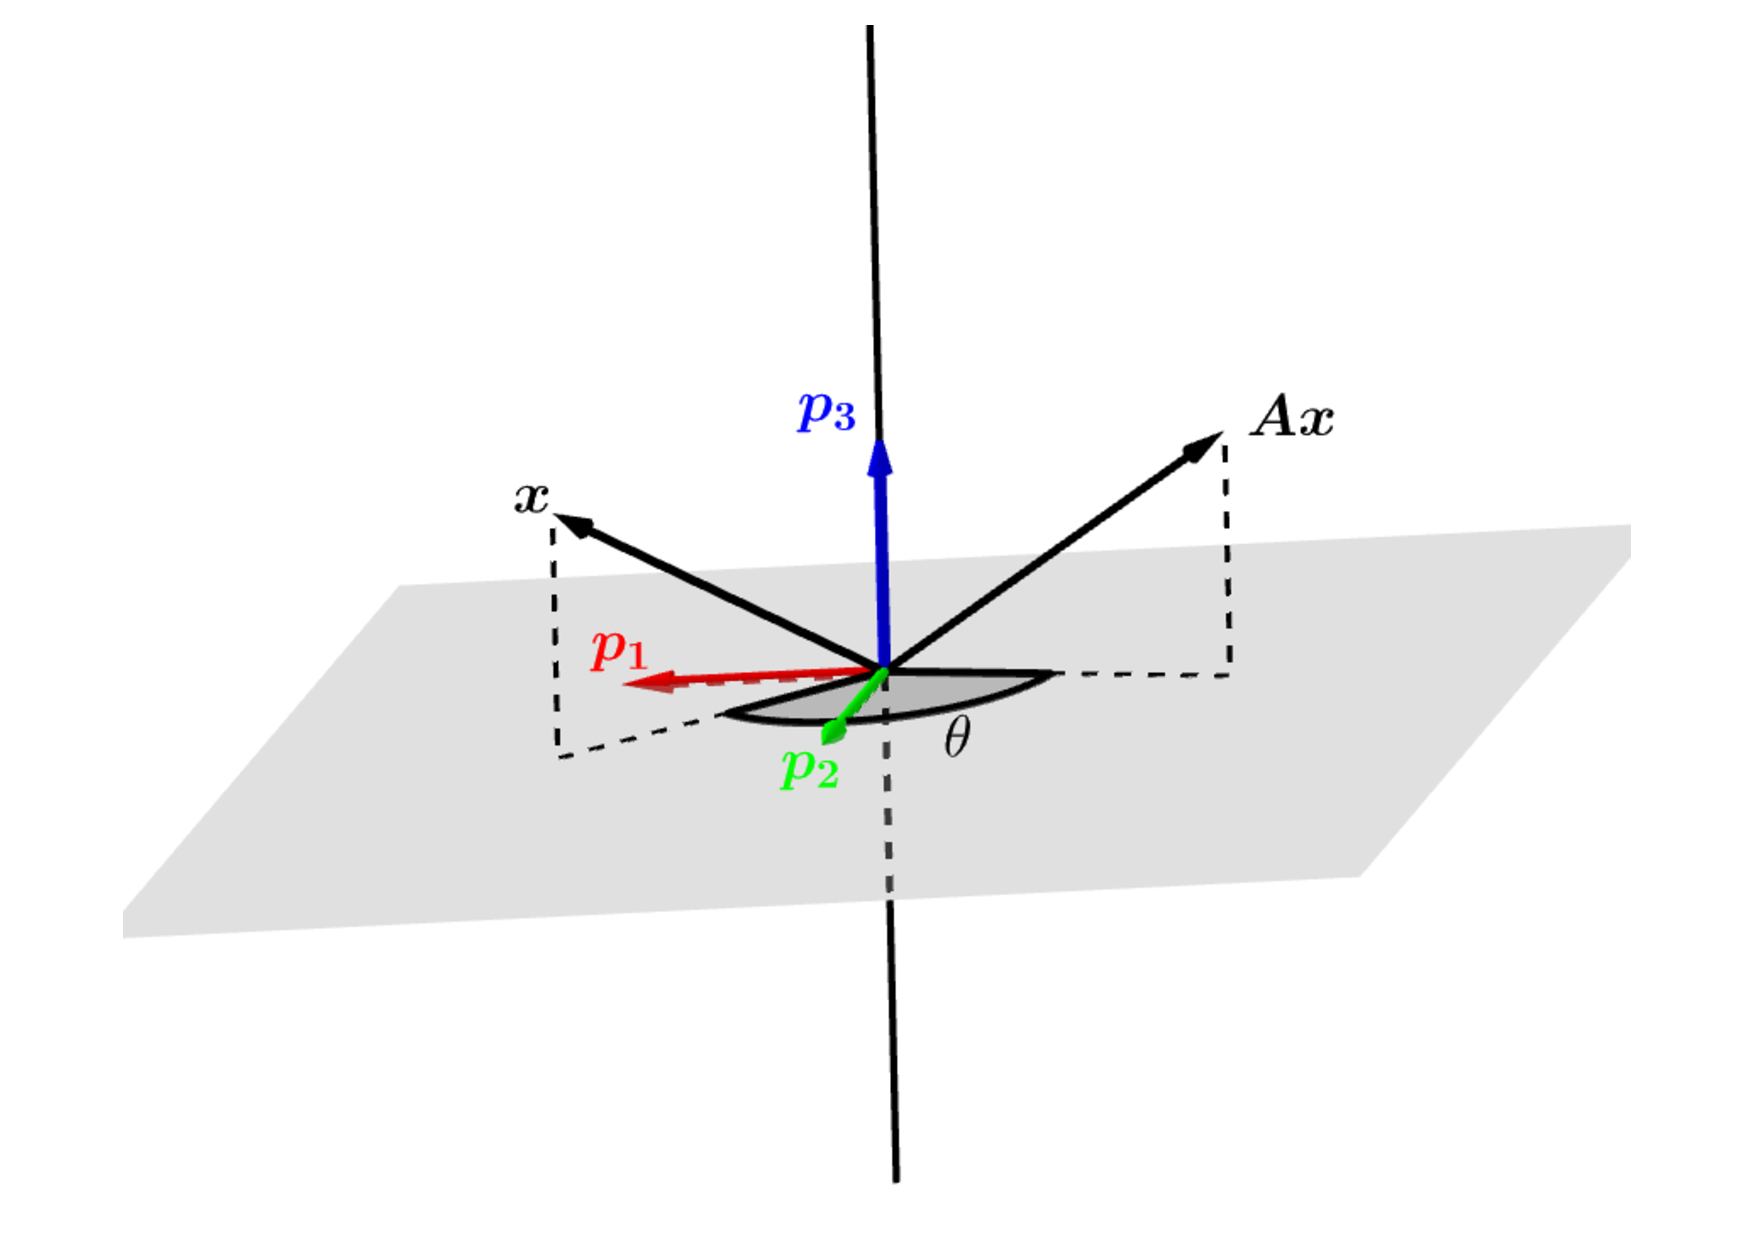
\includegraphics[height=4.3cm]{pictures/rotation3.pdf}
        \caption{$\bm{p}_3$ を軸とする回転角 $\theta$ の回転}\label{fig:rotation3}
      \end{minipage}
      \begin{minipage}{0.5\linewidth}
        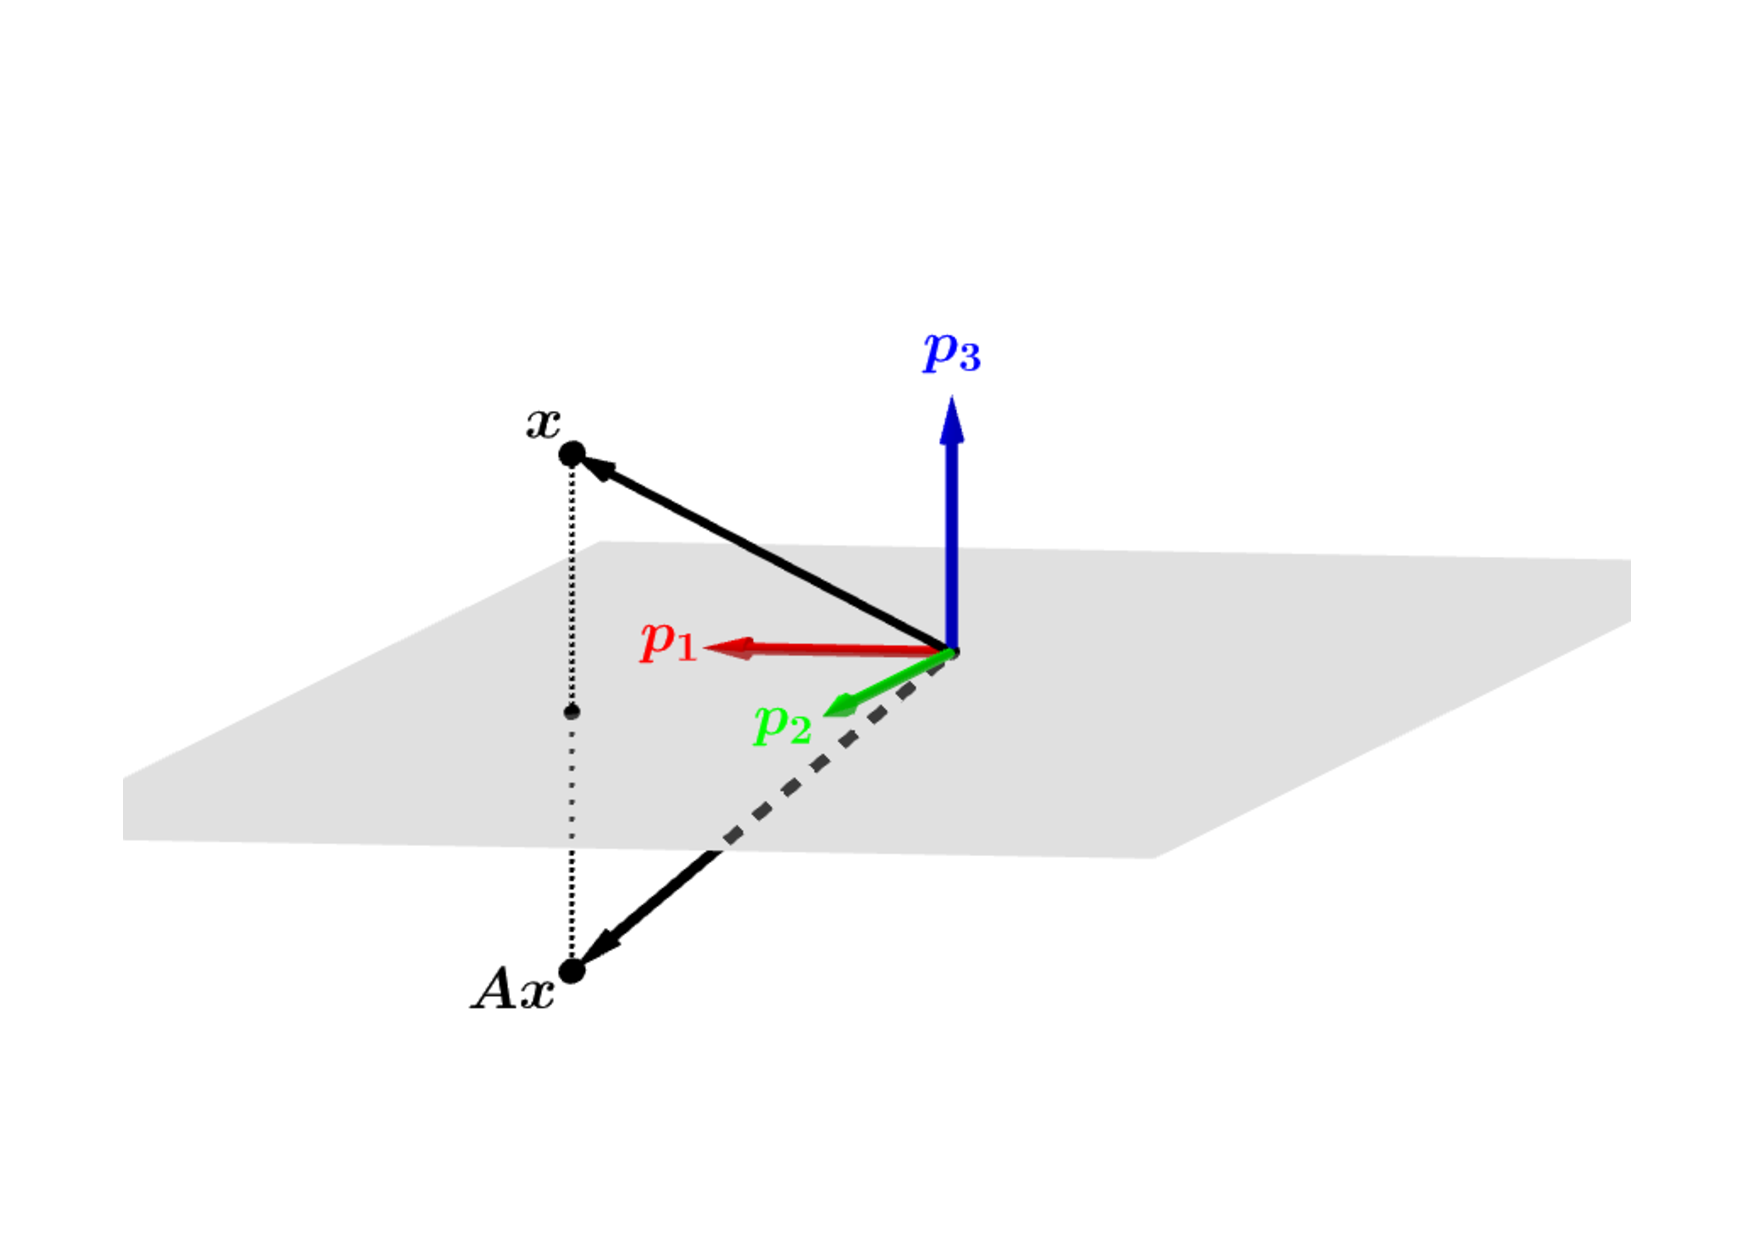
\includegraphics[height=4.3cm]{pictures/reflection3.pdf}
        \caption{平面 $\langle \bm{p}_1, \bm{p}_2\rangle$ に関する鏡映}\label{fig:reflection3}      
      \end{minipage}
    \end{tabular}
  \end{figure}


\end{itemize}

また,$3$ 次直交行列の標準形同士は以下の関係式を満たす.特
に,$S_{\theta}= R_{\theta}R_{0}, \; R_0^2=E$ である.
\[
  S_{\theta} S_{\phi} = R_{\theta}R_{\phi}=S_{\theta+\phi}, \quad  
  S_{\theta}R_{\phi} = R_{\phi}S_{\theta} = R_{\theta+\phi}
\]

\newpage

\subsection{空間の合同変換の分類}

空間 $\mathbb{R}^3$ の合同変換
\[
  f(\bm{x}) = A\bm{x} + \bm{b}
\]
は直交行列 $A$ の標準形と$3$ 次列ベクトル $\bm{b}$ によって
表\ref{tab:classification3}のように $7$ 種に分類できる.定
理\ref{thm:generate3}で示すように,$\mathbb{R}^3$ の合同変換は $4$ 個以
下の鏡映の合成として表せる.表\ref{tab:classification3}の4列目はその鏡
映の最小個数を表している.

\begin{table}[h]
  \centering
  \begin{tabular}[h]{|c|c|c|c|c|}\hline
    名前 & $A$ の標準形 & $\bm{b}$ & 鏡映の個数 & 固定点集合\\ \hline
    恒等変換 & $E$ & $\bm{0}$ & 0 & $\mathbb{R}^3$\\ 
    平行移動 & $E$ & $\bm{b} \neq \bm{0}$ & $2$ & 空集合\\
    回転 & $S_{\theta} (\neq E)$ & $\bm{b} \in V_{A}(1)^{\perp}$  & $2$ & 回転軸\\
    螺旋運動 & $S_{\theta} (\neq E)$ & $\bm{b} \notin V_{A}(1)^{\perp}$ & $4$ &  空集合\\ 
    鏡映 & $R_{0}$ & $\bm{b} \in V_A(-1)$ & $1$ & 鏡映面\\
    滑り鏡映 & $R_{0}$ & $\bm{b} \notin V_A(-1)$ & $3$ & 空集合\\
    回転鏡映 & $R_{\theta} (\neq R_{0})$ & $\bm{b} \in \mathbb{R}^3$ & $3$ &  中心点\\ \hline    
  \end{tabular}
  \caption{空間 $\mathbb{R}^3$ の合同変換の分類表}
  \label{tab:classification3}
\end{table}

ここでは,実際に $\mathbb{R}^3$ の合同変
換 $f$ が表\ref{tab:classification3}のいずれかに分類され,またそれで全
てであることを確かめていこう.恒等変換と平行移動に関しては明らかなので,
以下 $f$ は恒等変換でも平行移動でもない,すなわち,$A \neq E$ とする.


\subsubsection{回転と螺旋運動}\label{sec:RotSpiral3}

$A \sim S_{\theta}$ かつ $A \neq E$ とする.このとき,$f$ は回転か螺旋
運動である.これを詳しく見ていこう.なお,空間における螺旋運動の定義は
以下の通りである.

\begin{definition}
  空間内の直線 $L$ を軸とする角 $\theta$ の回転 $g$ と $L$ に平行なベク
  トル $\bm{c} \in \mathbb{R}^3$ による平行移動との合
  成 $t_{\bm{c}}\circ g$ を $L$ と $\bm{c}$ に関する角 $\theta$ の螺旋
  運動という.この定義に従えば螺旋運動は回転($\bm{c}=\bm{0}$ のとき)を含むのだが,本
  稿では回転でないもののみを螺旋運動と呼ぶことにする.
\end{definition}


直交行列 $A$ が直交行列 $P \in SO(3)$ によって標
準化される,すなわち,
\[
  S_{\theta} = P^{-1}AP = {}^{t}P A P, \quad P=\left[
    \begin{array}{ccc}
      \bm{p}_1 & \bm{p}_2 & \bm{p}_3
    \end{array}
  \right] \in SO(3)
\]
とする.$\det P=1$ なので $\left( \bm{p}_1, \bm{p}_2, \bm{p}_3\right)$
は $\mathbb{R}^3$ の右手系正規直交基底であり,
\[
  V_A(1)= \langle \bm{p}_3 \rangle, \quad V_A(1)^{\perp} = \langle \bm{p}_1, \bm{p}_2 \rangle
\]
である.このとき,次が成り立つ.

\begin{theorem}\label{thm:RotOrSpiral3}
  $A,\bm{p}_1, \bm{p}_2, \bm{p}_3$ を先の通りとする.このとき,合同変
  換 $f(\bm{x}) = A\bm{x} + \bm{b}$ は回転か螺旋運動である.特に,各々
  の詳細は次の通りである.
  \begin{enumerate}[(1)]
  \item $\bm{b} \in V_A(1)^{\perp}$ のと
    き:固定点集合 $\Fix(f)$ は $V_A(1)=\langle \bm{p}_3\rangle$ に平行な直線であ
    り,$f$ はこの直線を軸とする回転角 $\theta$ の回転である.
    
  \item $\bm{b} \not\in V_A(1)^{\perp}$ のとき: $f$ は固定点を持な
    い.$f$ は回転 $g(\bm{x}) = A\bm{x} +
    \bm{b}-(\bm{b} \cdot \bm{p}_3)\bm{p}_3$ の軸とベクトル
    $(\bm{b}\cdot \bm{p}_3)\bm{p}$ による平行移動に関する角 $\theta$ の螺
    旋運動である.このとき,$g$ の回転軸 $\Fix(g)$ は $V_A(1)=\langle
    \bm{p}_3 \rangle$ に平行である.
  \end{enumerate}
  ただし,いずれも回転の向きは $\bm{p}_3$ の方向に進む右ねじの回転方向
  を正とする.
\end{theorem}

以下,定理\ref{thm:RotOrSpiral3}を証明していこう.

まず,$f$ が固定点を持つかどうかは $\bm{b} \in V_A(1)^{\perp}$ か否かで
分かれる.つまり,次が成り立つ.

\begin{lemma}\label{lem:RotOrSpiral3}
  上の状況において,$\Fix(f)$ は $\bm{b} \in V_A(1)^{\perp}$ のとき,そ
  のときに限り,空集合でない.
\end{lemma}

\begin{proof}
  $\bm{b} \in V_A(1)^{\perp}$ とする.$\mathbb{R}^3$ の線形変
  換 $g(\bm{x}) = \bm{x}-A\bm{x}$ を考える.任意の $\bm{x} \in
  \mathbb{R}^3$ に対して
  \[
    g(\bm{x}) \cdot  \bm{p}_3 = \bm{x}\cdot \bm{p}_3 - (A\bm{x})\cdot \bm{p}_3 =
    \bm{x}\cdot \bm{p}_3 -(A\bm{x}) \cdot (A\bm{p}_3) =\bm{x} \cdot \bm{p}_3 -
    \bm{x}\cdot \bm{p}_3 = 0
  \]
  であるから,$g(\mathbb{R}^3) \subset \langle \bm{p}_3
  \rangle^{\perp}=V_A(1)^{\perp}=\langle \bm{p}_1, \bm{p}_2\rangle$
  である.さらに,$\ker g = V_A(1)$ なので線形変換の次元定理より
  \[
    \dim g(\mathbb{R}^3) = \dim \mathbb{R}^3 - \dim \ker g = 3 -1 =2
  \]
  であるから,$g(\mathbb{R}^3) = V_A(1)^{\perp}$ である.よっ
  て,$\bm{b} = g(\bm{c}) = \bm{c} - A\bm{c}$ となる
  $\bm{c} \in \mathbb{R}^3$ が存在する.すなわち,$\bm{c} \in \Fix(f)$
  なので $\Fix(f)$ は空集合でない.

  逆に,$\Fix(f)$ が空集合でないとする.任意の $\bm{x} \in \Fix(f)$ に対し
  て, $\bm{b} = \bm{x} - A\bm{x}$ だから
  \[
    \bm{b}\cdot \bm{p}_3 = \bm{x} \cdot \bm{p}_3 - (A\bm{x})\cdot  \bm{p}_3
    =\bm{x} \cdot \bm{p}_3 - (A\bm{x})\cdot ( A\bm{p}_3)
    =\bm{x}\cdot  \bm{p}_3 - \bm{x}\cdot  \bm{p}_3 = 0
  \]
  である.従って,$\bm{b} \in V_A(1)^{\perp}$ である.
\end{proof}

\begin{proof}[定理\ref{thm:RotOrSpiral3}の証明]

  \begin{enumerate}[(1)]
  \item $\bm{b} \in V_A(1)^{\perp}$ とする.補
    題\ref{lem:RotOrSpiral3}より $\Fix(f)$ は空集合でない.さら
    に,$\dim V_A(1)=1$ なので\ref{sec:inv3}節で見たよう
    に $\Fix(f)$ は $V_A(1)$ と平行な直線である.このとき,任意
    の $\bm{c} \in \Fix(f)$ と任意の $\bm{x} \in \mathbb{R}^3$ に対して
    \[
      f(\bm{x}) - \bm{c} = A(\bm{x}-\bm{c})
    \]
    である.よって,$f$ は $V_A(1)$ に平行な直線 $\Fix(f)$ を軸とする回
    転角 $\theta$ の回転である(図\ref{fig:rotation3gen}).ただし,回
    転の向きは $\bm{p}_3$ の方向に進む右ねじの回転方向を正とする.また,
    これより
    \[
      f= t_{\bm{c}} \circ T_A \circ t_{-\bm{c}} 
    \]
    とも表せる.すなわち,$\bm{c}$ を通る直線 $L$ を軸とする回転は「一
    旦 $-\bm{c}$ 平行移動し,原点を通り $\Fix(f)$ に平行な直線を軸とし
    て回転させた後に再び $\bm{c}$ 平行移動する変換」とも言い換えるられ
    る.
    \begin{figure}[h]
      \centering
      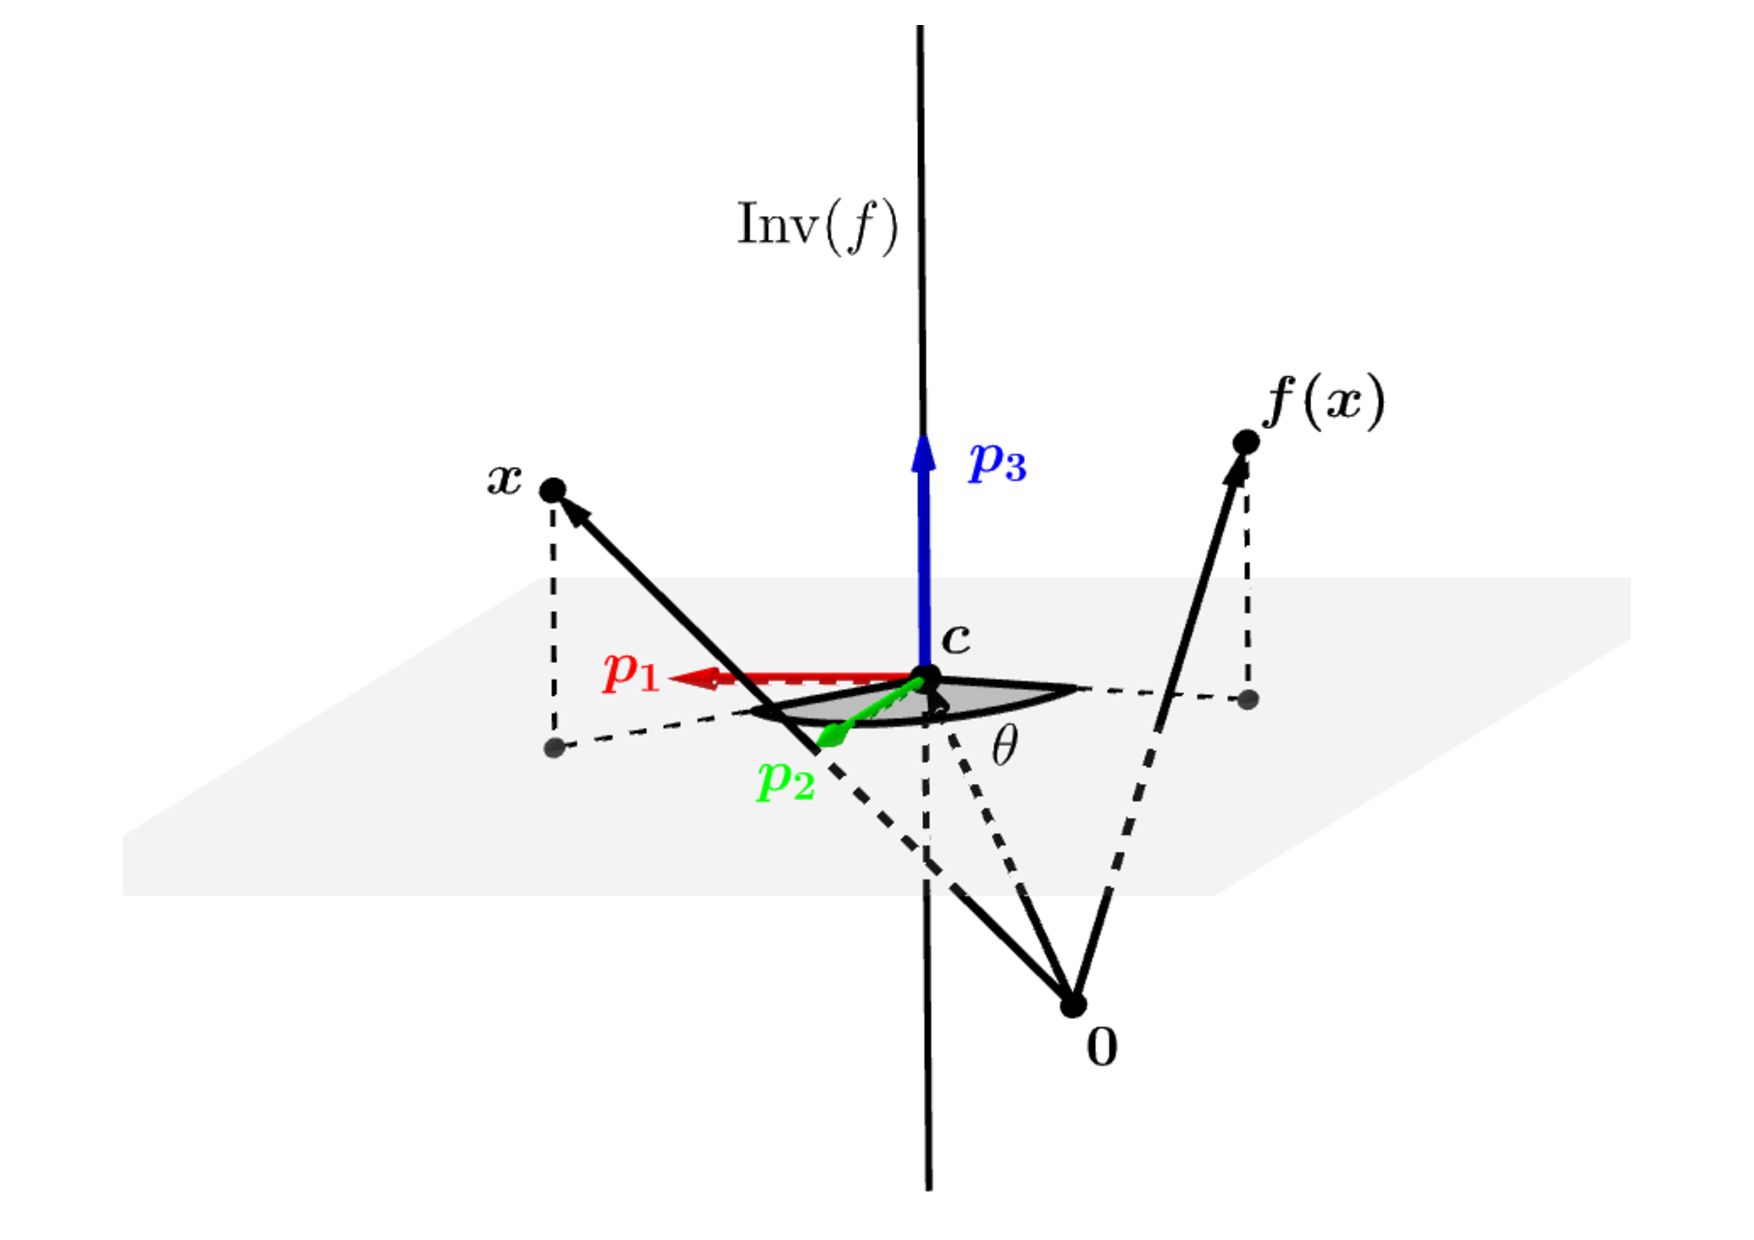
\includegraphics[height=4.5cm]{pictures/rotation3gen.pdf}
           \caption{直線 $\Fix(f)$ を軸とする角度 $\theta$ の回転}
      \label{fig:rotation3gen}
    \end{figure}

  \item $\bm{b} \notin V_A(1)^{\perp}$ とする.補
    題\ref{lem:RotOrSpiral3}より $f$ は固定点を持たない.このと
    き $\bm{b}$ を
    \[
      \bm{b} = \bm{b}_{12} + \bm{b}_3 , \quad \bm{b}_{12} \in
      V_A(1)^{\perp}=\langle \bm{p}_1, \bm{p}_2 \rangle, \; \bm{b}_{3} \in
      V_A(1)=\langle \bm{p}_3\rangle
    \]
    と分解すると,$\bm{b}_{12} \neq \bm{0}$ である.従って,
    \[
      f(\bm{x}) = \left( A\bm{x} + \bm{b}_{12}\right) + \bm{b}_3
    \]
    より $f$ は合同変換 $g(\bm{x}) = A\bm{x} + \bm{b}_{12}$ と平行移
    動 $t_{\bm{b}_3}$ の合成 $t_{\bm{b}_{3}} \circ g$ である(
    図\ref{fig:spiral3}).(1)より $g$ は直線 $\Fix(g)$ を軸とす
    る $\theta$ 回転であり,$\bm{b}_3 (\neq \bm{0})$ は $\Fix(g)$ と平
    行だから,$f$ は螺旋運動である.また,$(\bm{p}_1, \bm{p}_2,
    \bm{p}_3)$ は $\mathbb{R}^3$ の正規直交基底だから
    \[
      \bm{b}_{3} = (\bm{b}\cdot  \bm{p}_3) \bm{p}_3,\quad \bm{b}_{12} =
      \bm{b}-\bm{b}_{3} = \bm{b} - (\bm{b}\cdot \bm{p}_3)\bm{p}_3
    \]
    である.なお,
    \[
      g \circ t_{\bm{b}_3} (\bm{x}) = A(\bm{x} + \bm{b}_3) + \bm{b}_{12} =
      A\bm{x} + \bm{b}_3 + \bm{b}_{12} = f(\bm{x})
    \]
    より $t_{\bm{b}_3} \circ g = g \circ t_{\bm{b}_3} = f$ であるから合
    成の順番はどちらでもよい.
    \begin{figure}[h]
      \centering
      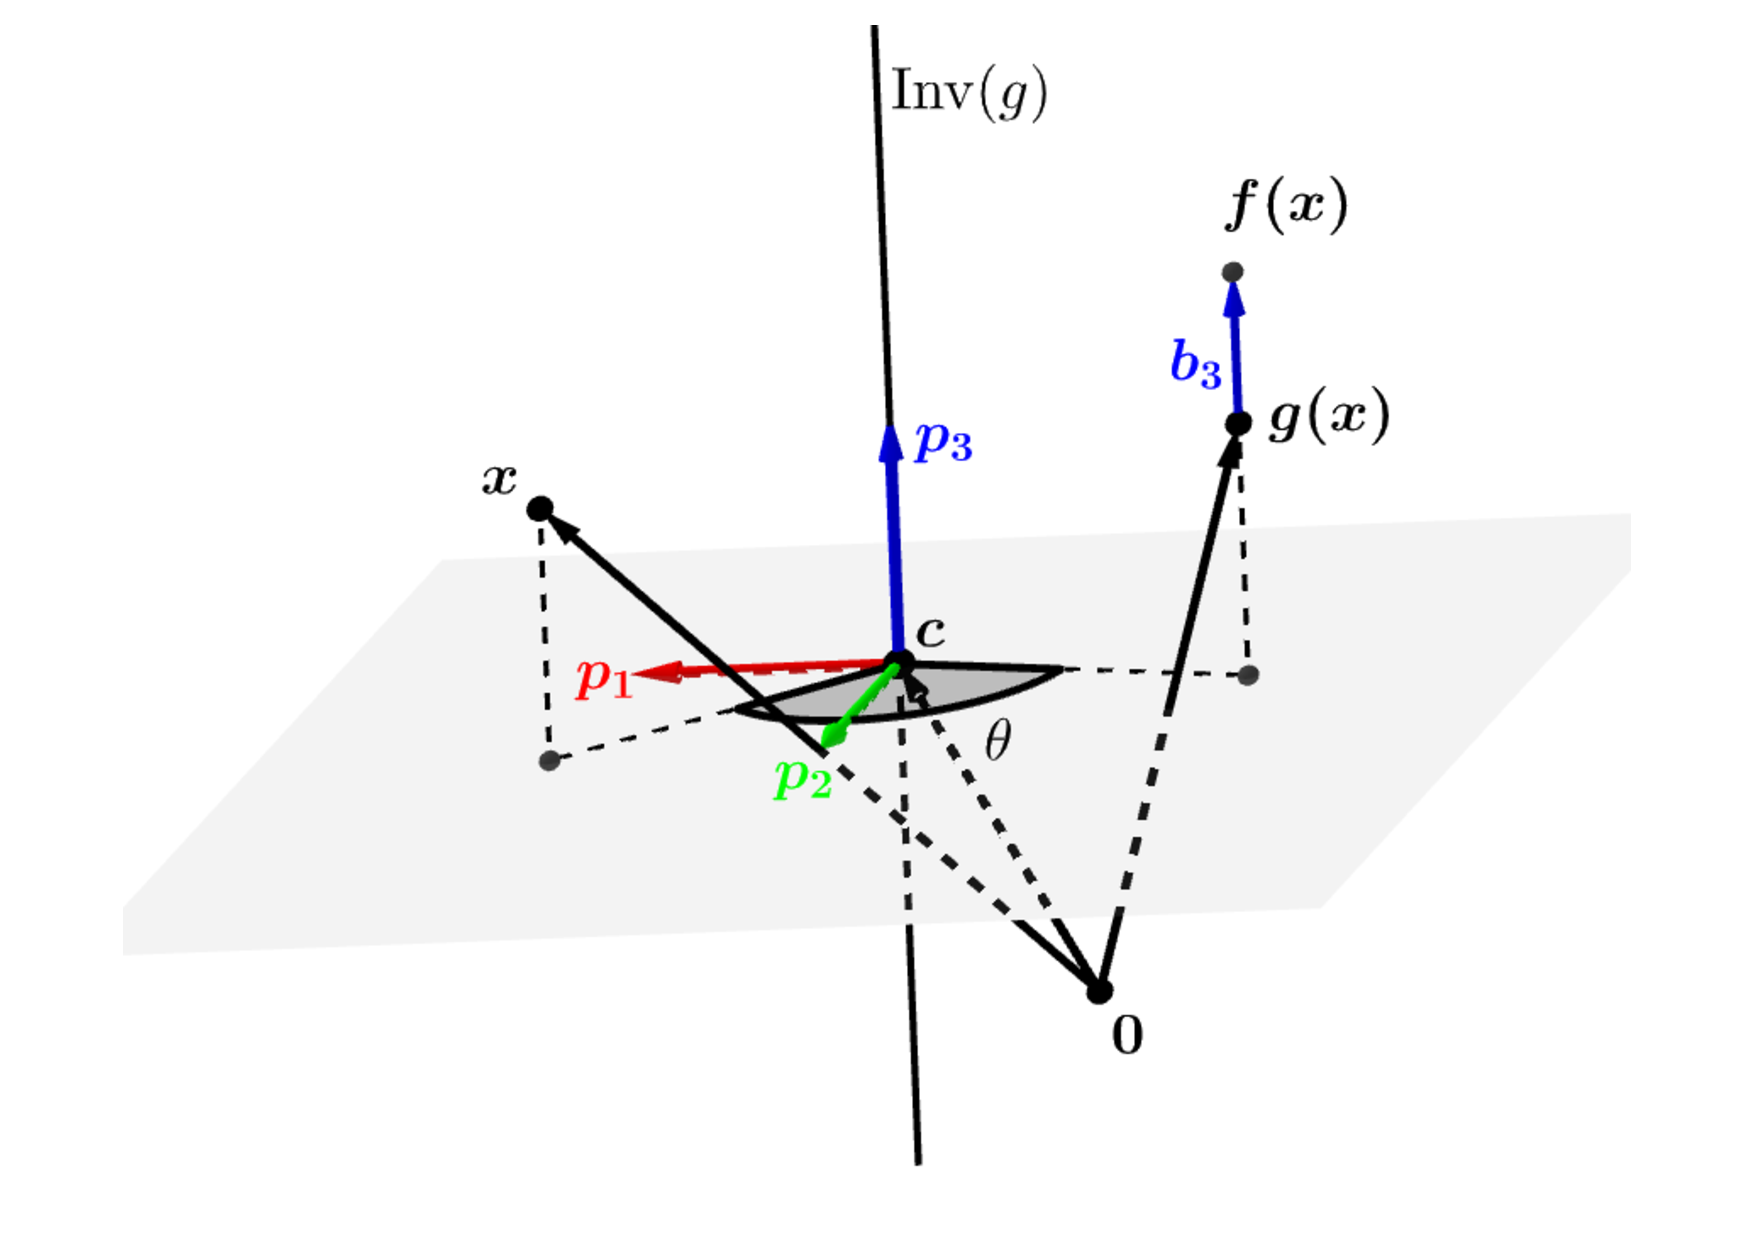
\includegraphics[height=4.5cm]{pictures/spiral3.pdf}
      \caption{$\Fix(g)$ と $\bm{b}_3$ に関する螺旋運動}
      \label{fig:spiral3}
    \end{figure}
  \end{enumerate}
\end{proof}

\subsubsection{鏡映と滑り鏡映}\label{sec:RefGlide3}

$A \sim R_0$ とする.このとき,$f$ は鏡映か滑り鏡映である.これを詳しく
見ていこう.なお,空間における滑り鏡映の定義は以下の通りである.

\begin{definition}
  空間内の平面 $H$ に関する鏡映 $g$ と $H$ に平行なベクトル $\bm{c}
  \in \mathbb{R}^3$ による平行移動との合成 $t_{\bm{c}} \circ
  g$ を $H$と $\bm{c}$ に関する滑り鏡映という.この定義に従えば滑り鏡映
  は鏡映($\bm{c}=\bm{0}$ のとき)を含むのだが,本稿では鏡映でないもの
  のみを滑り鏡映と呼ぶことにする.
\end{definition}


直交行列 $A$ が直交行列 $P \in SO(3)$ によって $R_{0}$ に標準化される,すなわち,
\[
  R_{0} = P^{-1}AP = {}^{t}PAP, \quad P=\left[
    \begin{array}{ccc}
      \bm{p}_1 & \bm{p}_2 & \bm{p}_3
    \end{array}
  \right] \in SO(3)
\]
とする.$A$ の固有値は $-1$ と $1$ である.$\det P=1$ なの
で $(\bm{p}_1, \bm{p}_2, \bm{p}_3)$ は $\mathbb{R}^3$ の右手系正規直交
基底であり,
\[
  V_A(-1) = \langle \bm{p}_3\rangle, \quad V_A(-1)^{\perp} = V_A(1)
  =\langle \bm{p}_1, \bm{p}_2 \rangle
\]
である.このとき,次が成り立つ.

\begin{theorem}\label{thm:RefOrGlide3}
  $A, \bm{p}_1, \bm{p}_2, \bm{p}_3$ を上の通りとする.このとき,合同変
  換 $f(\bm{x}) = A\bm{x} + \bm{b}$ は鏡映か滑り鏡映である.特に,各々
  の詳細は次の通りである.
  \begin{enumerate}[(1)]
  \item $\bm{b} \in V_A(-1)$ のとき:固定点集
    合 $\Fix(f)$ は $\bm{b}/2$ を通り $V_A(1)$ に平行な平面であり,$f$
    はこの平面に関する鏡映である.

  \item $\bm{b} \not\in V_A(-1)$ のとき:$f$ は固定点を持たない.$f$ は
    鏡映 $g(\bm{x})=A\bm{x} + (\bm{b}\cdot \bm{p}_3)\bm{p}_3$ とベクト
    ル $\bm{b}-(\bm{b}\cdot \bm{p}_3)\bm{p}_3$ の鏡映面 $\Fix(g)$ に関
    する滑り鏡映である.このとき,$g$ は $(\bm{b}\cdot
    \bm{p}_3)\bm{p}_3/2$ を通り $V_A(1)$ に平行な平面に関する鏡映であ
    る.
  \end{enumerate}
\end{theorem}

以下,定理\ref{thm:RefOrGlide3}を証明していこう.

まず,$f$ が固定点を持つかどうかは $\bm{b} \in V_A(-1)$ か否かで分かれ
る.つまり,次が成り立つ.

\begin{lemma}\label{lem:RefOrGlide3}
  上の状況において,$\Fix(f) \neq \emptyset$ であることと $\bm{b} \in
  V_A(-1)$ であることは同値である.
\end{lemma}

\begin{proof}
  直交行列 $A$ による固有空間分解 $\mathbb{R}^3 = V_A(1) \oplus V_A(-1)$ に
  よって $\bm{b}$ を次のように分解する.
\[
  \bm{b} = \bm{b}^{+} + \bm{b}^{-}, \quad \bm{b}^{+}   \in V_A(1), \; \bm{b}^{-}  \in V_A(-1)
\]

まず,$\Fix(f) \neq \emptyset$ とする.$x \in \Fix(f)$
に対して $f(\bm{x}) = \bm{x}$ なので
\begin{equation}\label{eq:xinFix3}
  A \bm{x} + \bm{b}^{+} + \bm{b}^{-} = x
\end{equation}
である.$A^2=PR_0^2P^{-1} = E, \; A\bm{b}^{\pm} = \pm
\bm{b}^{\pm}$ なので,この (\ref{eq:xinFix3}) の両辺に左から $A$ を掛けて
\begin{equation}\label{eq:AxinFix3}
  \bm{x}  + \bm{b}^{+} - \bm{b}^{-} = A\bm{x}
\end{equation}
が得られる.これ
ら (\ref{eq:xinFix3}) と (\ref{eq:AxinFix3}) から $\bm{b}^{+}=\bm{0}$
より, $\bm{b} \in V_A(-1)$ である.

逆に,$\bm{b} \in V_A(-1)$ とする.$A\bm{b} = -\bm{b}$ なので
\[
  f\left(\frac{\bm{b}}{2}\right) = A\left(\frac{\bm{b}}{2}\right)
  +\bm{b} = -\frac{\bm{b}}{2} + \bm{b} = \frac{\bm{b}}{2}
\]
より, $\bm{b}/2 \in \Fix(f)$ だから $\Fix(f) \neq \emptyset$ である.


あるいは,$V_A(-1)= V_A(1)^{\perp}$ なので補題\ref{lem:RotOrSpiral3}と
同様の議論によって示すこともできる.
\end{proof}

\begin{proof}[定理\ref{thm:RefOrGlide3}の証明]
  
  \begin{enumerate}[(1)]
  \item $\bm{b} \in V_A(-1)$ とする.補
    題\ref{lem:RefOrGlide3}より $\Fix(f)$は空集合でない.$\dim
    V_A(1)=2$ なので\ref{sec:inv3}節で見たよう
    に $\Fix(f)$ は $V_A(1)$ と平行な平面である.特に,
    \[
      f\left(\frac{\bm{b}}{2}\right) = A\left(\frac{\bm{b}}{2}\right)
      + \bm{b} = -\frac{\bm{b}}{2} + \bm{b} = \frac{\bm{b}}{2}
    \]
    より,$\bm{b}/2 \in \Fix(f)$ だから $\Fix(f)$ は $\bm{b}/2$ を通
    る.$f$ は平面 $\Fix(f)$ に関する鏡映である.実際,任意の $\bm{x}
    \in \mathbb{R}^3$ と任意の $\bm{p} \in V_A(1)$ に対して,
    \begin{align*}
      \left(f(\bm{x})-\bm{x}\right)\cdot  \bm{p} &= (A\bm{x})\cdot  \bm{p} + \bm{b}\cdot \bm{p}
                                                   - \bm{x}\cdot \bm{p}
      =(A\bm{x})\cdot ( A\bm{p}) - \bm{x}\cdot \bm{p} = \bm{x}\cdot \bm{p} - \bm{x}\cdot \bm{p} =0,\\
      f\left(\frac{f(\bm{x})+\bm{x}}{2}\right) &= A\left( \frac{A\bm{x}+\bm{b}+\bm{x}}{2}\right)+\bm{b}
      = \frac{\bm{x}-\bm{b}+A\bm{x}}{2} + \bm{b} 
      = \frac{A\bm{x}+\bm{b}+\bm{x}}{2} = \frac{f(\bm{x})+\bm{x}}{2}
    \end{align*}
    であるから,$f(\bm{x})-\bm{x}$ が $V_A(1)$ に,従って $\Fix(f)$ に,
    直交し,$f(\bm{x})$ と $\bm{x}$ の中点が $\Fix(f)$ 上にあるの
    で,$f$ は平面 $\Fix(f)$ に関する鏡映である.



    また,任意の $\bm{c} \in \Fix(f)$ と任意
    の $\bm{x} \in \mathbb{R}^3$ に対し
    \[
      f(\bm{x}) = A(\bm{x}-\bm{c}) + \bm{c}
    \]
    が成り立つから
    \[
      f=t_{\bm{c}} \circ T_A \circ t_{-\bm{c}}
    \]
    である.すなわち,$\bm{c}$ を通り平面 $V_A(1)$ に平行な平面に関する鏡映
    は「一旦 $-\bm{c}$ 平行移動し,$V_A(1)$ に関する鏡映移動をした後に再
    び $\bm{c}$ 平行移動する変換」と言い換えることもできる.

  \item $\bm{b} \notin V_A(-1)$ とする.空間 $\mathbb{R}^3$ の固有分
    解 $\mathbb{R}^3 = V_A(1) \oplus V_A(-1)$ により $\bm{b}$ を
    \[
      \bm{b} = \bm{b}^{+} + \bm{b}^{-}, \quad \bm{b}^{+} \in V_A(1),
      \; \bm{b}^{-} \in V_A(-1)
    \]
    と分解する.このとき,$\bm{b}^{+} \neq \bm{0}$ である.
    \[
      f(\bm{x}) = \left(A\bm{x} + \bm{b}^{-}\right) + \bm{b}^{+}
    \]
    であるから,$g(\bm{x}) = A\bm{x} + \bm{b}^{-}$
    とおくと,$f = t_{\bm{b}^{+}} \circ g$ であ
    る.(1)より $g$ は $\bm{b}^{-}$ を通り $V_A(1)$ に平行な平
    面 $\Fix(g)$ に関する鏡映である.さらに,$\bm{b}^{+} \in V_A(1)$ で
    あるから $\bm{b}^{+}$ は $\Fix(g)$ に平行である.よって,$f$ は滑り
    鏡映である.また,$(\bm{p}_1, \bm{p}_2,
    \bm{p}_3)$ は $\mathbb{R}^3$ の正規直交基底だから
    \[
      \bm{b}^{-} = (\bm{b}\cdot \bm{p}_3)\bm{p}_3, \quad
      \bm{b}^{+}=\bm{b}-\bm{b}^{-}=\bm{b}-(\bm{b}\cdot \bm{p}_3)\bm{p}_3
    \]
    である.なお,鏡映と平行移動を合成する順番はどちらでもよい.実
    際,$A\bm{b}^{+}=\bm{b}^{+}$ より
    \[
      g\left(t_{\bm{b}^{+}}(\bm{x})\right) = A\left(\bm{x}+\bm{b}^{+}\right)+\bm{b}^{-}
      = \left(A\bm{x}+\bm{b}^{-}\right) + \bm{b}^{+} = t_{\bm{b}^{+}}\left( g(\bm{x})\right)
    \]
    であるから $g\circ t_{\bm{b}^{+}} = t_{\bm{b}^{+}}\circ g=f$ である.
  \end{enumerate}
\end{proof}


\subsubsection{回転鏡映}

$A \sim R_{\theta} \neq R_0$ とする.このとき $f$ は回転鏡映である.こ
れを詳しく見ていこう.

直交行列 $A$ が直交行列 $P \in SO(3)$ によって $R_{\theta}$ に標準化される,すなわち,
\[
  R_{\theta}=P^{-1}AP = {}^{t}PAP, \quad P=\left[
    \begin{array}{ccc}
      \bm{p}_1 & \bm{p}_2 & \bm{p}_3
    \end{array}
  \right] \in SO(3)
\]
とする.$\det P=1$ なので $(\bm{p}_1, \bm{p}_2,
\bm{p}_3)$ は $\mathbb{R}^3$ の右手系正規直交基底であり,
\[
  V_A(-1) = \langle \bm{p}_3\rangle, \quad V_A(-1)^{\perp}=\langle
  \bm{p}_1, \bm{p}_2\rangle
\]
である.このとき,次が成り立つ.

\begin{theorem}\label{thm:rotref3}
  $A, P, \bm{p}_1, \bm{p}_2, \bm{p}_3$ を上の通りとする.このとき,合同
  変換 $f(\bm{x}) = A\bm{x}+\bm{b}$ は回転鏡映である.特に,固定点
  は $1$ 点 $\bm{c}:=(E-A)^{-1}\bm{b}$ のみであり,$f$ は $V_A(-1)$ に
  平行で $\bm{c}$ を通る直線に関する $\theta$ 回転 $g$ と $\bm{c}$ を通
  り $V_A(-1)^{\perp}$ に平行な平面に関する鏡映 $h$ の合成 $g \circ h$
  に等しい.ただし,回転の向きは $\bm{p}_3$ の向きに進む右ねじの回転方
  向を正とする.
\end{theorem}

\begin{remark}
  この定理は幾何学的には明らかだが,ここでは(線形)代数的にきっちり証明して
  いこう.  
\end{remark}

\begin{proof}
$R_{\theta}=S_{\theta}R_{0}$ であるから,$B=PS_{\theta}P^{-1}, \; C=PR_{0}P^{-1}$ とおくと
\[
  BC = \left(PS_{\theta}P^{-1}\right)\left(PR_{0}P^{-1}\right) = P
  \left( S_{\theta}R_{0}\right)P^{-1} = P R_{\theta} P^{-1}=A
\]
である.$\mathbb{R}^3$ の直交分解 $\mathbb{R}^3 = V_B(1) \oplus
V_B(1)^{\perp}$ によって $\bm{b}$ を
\[
  \bm{b}=\bm{b}_{1} + \bm{b}_{2}, \quad \bm{b}_{1} \in
  V_B(1), \; \bm{b}_2 \in V_B(1)^{\perp}
\]
と分解する.$B \bm{b}_1 = \bm{b}_1$
だから,$g(\bm{x}) = B\bm{x} + \bm{b}_{2}, \; h(x) = C\bm{x}+\bm{b}_1$
とおくと
\[
  f(\bm{x}) = A\bm{x} + \bm{b} = BC\bm{x}+\bm{b}_{1}+\bm{b}_{2} =
  B\left(C\bm{x}+\bm{b}_{1}\right) + \bm{b}_{2} = g(h(\bm{x}))
\]
より,$f= g \circ h$ である.$B, C$ はいずれも $P$ によってそれ
ぞれ $S_{\theta}, \; R_0$ に標準化されるので
\[
  V_A(-1) = \langle \bm{p}_3 \rangle = V_B(1)=V_C(-1), \quad
  V_A(-1)^{\perp} = \langle \bm{p}_1, \bm{p}_2\rangle = V_B(1)^{\perp}
  = V_C(-1)^{\perp}=V_C(1)
\]
である.これより $g(\bm{x})=B\bm{x}+\bm{b}_2$ が回転
で,$h(\bm{x})=C\bm{x}+\bm{b}_1$ が鏡映であることを示せばよい.


まず,$B \sim S_{\theta} \neq E$ かつ $\bm{b}_{2} \in V_B(1)^{\perp}$
だから,定理\ref{thm:RotOrSpiral3}より $\Fix(g)$ は $V_B(1)=V_A(-1)$ に
平行な直線で,$g$ はこの直線に関する $\theta$ 回転である.ただし,回転
の向きは $\bm{p}_3$ の向きに進む右ねじの回転方向を正とする.

次に,$C \sim R_0$ かつ $\bm{b}_1 \in V_B(1)=V_C(-1)$ だから,定
理\ref{thm:RefOrGlide3}より $\Fix(h)$ は $V_C(1)=V_A(-1)^{\perp}$ に平
行な平面で,$h$ はこの平面に関する鏡映である.

最後に,$A$ は $1$ を固有値に持たないので\ref{sec:inv3}節で見たよう
に $f$ の固定点は $\bm{c}:=(E-A)^{-1}\bm{b}$ のみであるが,これ
は $\Fix(g)$ と $\Fix(h)$ の交点である.実際,空間 $\mathbb{R}^3$ の中
で直線 $\Fix(g)$ と平面 $\Fix(h)$ は直交するので $1$ 点で交わるが,その
交点は $g, h$ の固定点なので $f$ の固定点でもあり,従って,$\bm{c}$ に
等しい.よって,$\Fix(g)$ も $\Fix(h)$ も $\bm{c}$ を通る.
\end{proof}


\subsection{鏡映の個数}

空間の合同変換それぞれに対し,それを合成する鏡映を全て調べ上げ,分類
表\ref{tab:classification3}を完成させよう.

\begin{theorem}\label{thm:generate3}
  空間 $\mathbb{R}^3$ の合同変換は $4$ 個以
  下の鏡映の合成として表せる.特に,各合同変換に対してそれを合成
  する鏡映の最小個数は表\ref{tab:classification3}にある通りである.
\end{theorem}

定理の証明の前に,合同変換の合成と固定点集合に関する補題を与えておく.

\begin{lemma}\label{lem:inv-comp3}
  空間 $\mathbb{R}^3$ の任意の合同変換 $f_1,
  f_2$に対し,$ \Fix(f_1) \cap \Fix(f_2) \subset \Fix(f_1 \circ f_2)$
  が成り立つ.特に,$\Fix(f_1 \circ f_2)$ が空集合なら $\Fix(f_1) \cap
  \Fix(f_2)$ は空集合である.
\end{lemma}

\begin{proof}
  任意の $\bm{c} \in \Fix(f_1) \cap \Fix(f_2)$ に対して,以下が成り立つので $\bm{c} \in \Fix(f_1 \circ f_2)$ である.
  \[
    f_1 \circ f_2(\bm{c}) = f_1\left( f_2(\bm{c})\right) = f_1(\bm{c}) = \bm{c}
  \]
  よって,$\Fix(f_1) \cap \Fix(f_2) \subset \Fix(f_1 \circ f_2)$ である.
  後半の主張は明らかである.
\end{proof}


\begin{proof}[定理\ref{thm:generate3}の証明]
  恒等変換は $0$ 個,鏡映は $1$ 個の鏡映の合成であり,またそれ以外の合
  同変換が $1$ 個以下の鏡映の合成として表せないことは明らかである.残り
  の平行移動,回転,滑り鏡映,回転鏡映,螺旋運動に関しては以下に続く4つの補
  題\ref{lem:translation3}から\ref{lem:spiral3}により証明が完成す
  る.
\end{proof}


\begin{lemma}\label{lem:translation3}
  \begin{enumerate}[(1)]
  \item 空間 $\mathbb{R}^3$ の平行移動
    $t_{\bm{b}} \; (\bm{b} \neq \bm{0})$は鏡映面が平行な2個の鏡映の合成
    である.このとき,2つの鏡映面は共に $\bm{b}$ に直交し,その距離
    は $\|\bm{b}\|/2$ である.

\item 逆に,空間 $\mathbb{R}^3$ の平行な $2$ 平面 $H_1, H_2 \; (H_1
  \neq H_2)$ に関する鏡映$r_1, r_2$ の合成 $r_2 \circ r_1$は平行移動で
  ある.移動方向は $H_1$ から $H_2$ の方へ両平面に直交する方向で,移動
  距離は $2$ 平面の距離の $2$ 倍である.
  \end{enumerate}
\end{lemma}



\begin{proof}
  (1)原点 $\bm{0}$ と $t_{\bm{b}}(\bm{0})=\bm{b}$ の垂直二等分面 $H$ に
  関する鏡映を $g$ とする.$g(\bm{0})=\bm{b}$ だから,$g$ は
  $A \sim R_0, \; \bm{b} \in V_A(-1)$ を満たす $3$ 次直交行列 $A$ によっ
  て $g(\bm{x}) = A\bm{x} + \bm{b}$ と書ける.このとき,
  \[
    g\left( t_{\bm{b}}(\bm{x})\right) = A(\bm{x}+\bm{b})+\bm{b} =
    A\bm{x} + A\bm{b} + \bm{b} = A\bm{x} -\bm{b} +\bm{b}=A\bm{x} = T_A(\bm{x})
  \]
  より $g\circ t_{\bm{b}} = T_A$ である.$A \sim R_0$ だから直交変
  換 $T_A$ は平面 $H_0:=V_A(1)$ に関する鏡映である.さらに,$g\circ g =
  \id_{\mathbb{R}^3}$ より
  \[
    t_{\bm{b}}= \left( g \circ g\right) \circ t_{\bm{b}} = g\circ \left( g \circ t_{\bm{b}}\right) = g \circ T_A
  \]
  だから平行移動 $t_{\bm{b}}$ は $2$ 個の鏡映 $g$ と $T_A$ の合成である.
  また,$g$ の鏡映面 $H$ は $T_A$ の鏡映面 $H_0$ に平行であり,
  図\ref{fig:translation3}のように $H, H_0$ はそれぞれ $\bm{b}/2,
  \bm{0}$ を通り $\bm{b}$ に直交する平面なので,$2$ 平面間の距離
  は $\|\bm{b}\|/2$ である.
  % (1) 平行移動 $t_{\bm{b}} \; (\bm{b} \neq \bm{0})$ が $2$ 個の鏡映の合成で
  % あることを示す.
  % \[
  %   H_0:=\Set{ \bm{x} \in \mathbb{R}^3 | (\bm{b}, \bm{x})=0}
  % \]
  % とする.$H_0$ は原点 $\bm{0}$ を通り $\bm{b}$ に直交する平面であるか
  % ら,線形空間 $\mathbb{R}^3$ の $2$ 次元部分空間である.$(\bm{p}_1,
  % \bm{p}_2)$ を $H_0$ の正規直交基底とし,$\bm{p}_3 =
  % \bm{b}/\|\bm{b}\|$ とすると,$(\bm{p}_1, \bm{p}_2,
  % \bm{p}_3)$ は $\mathbb{R}^3$ の正規直交基底であるから,$P:=\left[
  %   \begin{array}{ccc}
  %     \bm{p}_1 & \bm{p}_2 & \bm{p}_3
  %   \end{array}
  % \right] \in O(3)$ である.$\det P =-1$ なら $\bm{p}_1$ と $\bm{b}_2$
  % を入れ替えて $P \in SO(3)$ とし,$A=P R_0 P^{-1}$ とする.$A \sim
  % R_0$ より直交変換 $T_A(\bm{x}) = A\bm{x}$ は平面
  % $V_A(1) = \langle \bm{p}_1, \bm{p}_2 \rangle = H_0$ に関する鏡映であ
  % る.$\bm{b} \in \langle \bm{p}_3 \rangle = V_A(-1)$ より,定
  % 理\ref{thm:RefOrGlide3}から合同変
  % 換 $g(\bm{x})=A\bm{x}+\bm{b}$ は $\bm{b}/2$ を通り $V_A(1)$ に平行な
  % 平面 $H:=\Fix(g)$ に関する鏡映である.よって,
  % \[
  %   t_{\bm{b}}(\bm{x}) = \bm{x} + \bm{b} = A\left( A\bm{x} \right) +
  %   \bm{b} = g\left( T_A(\bm{x})\right)
  % \]
  % より $t_{\bm{b}} = g \circ T_A$ である.すなわち,平行移
  % 動 $t_{\bm{b}}$ は平行な $2$ 平面 $H_0, H$ に関する $2$ 個の鏡映の合
  % 成である.このとき,$2$ 平面 $H_0, H$ の距離は原点 $\bm{0}$ と $H$ の
  % 距離 $\|\bm{b}\|/2$ に等しい(図\ref{fig:translation3}).
  \begin{figure}[h]
    \centering
    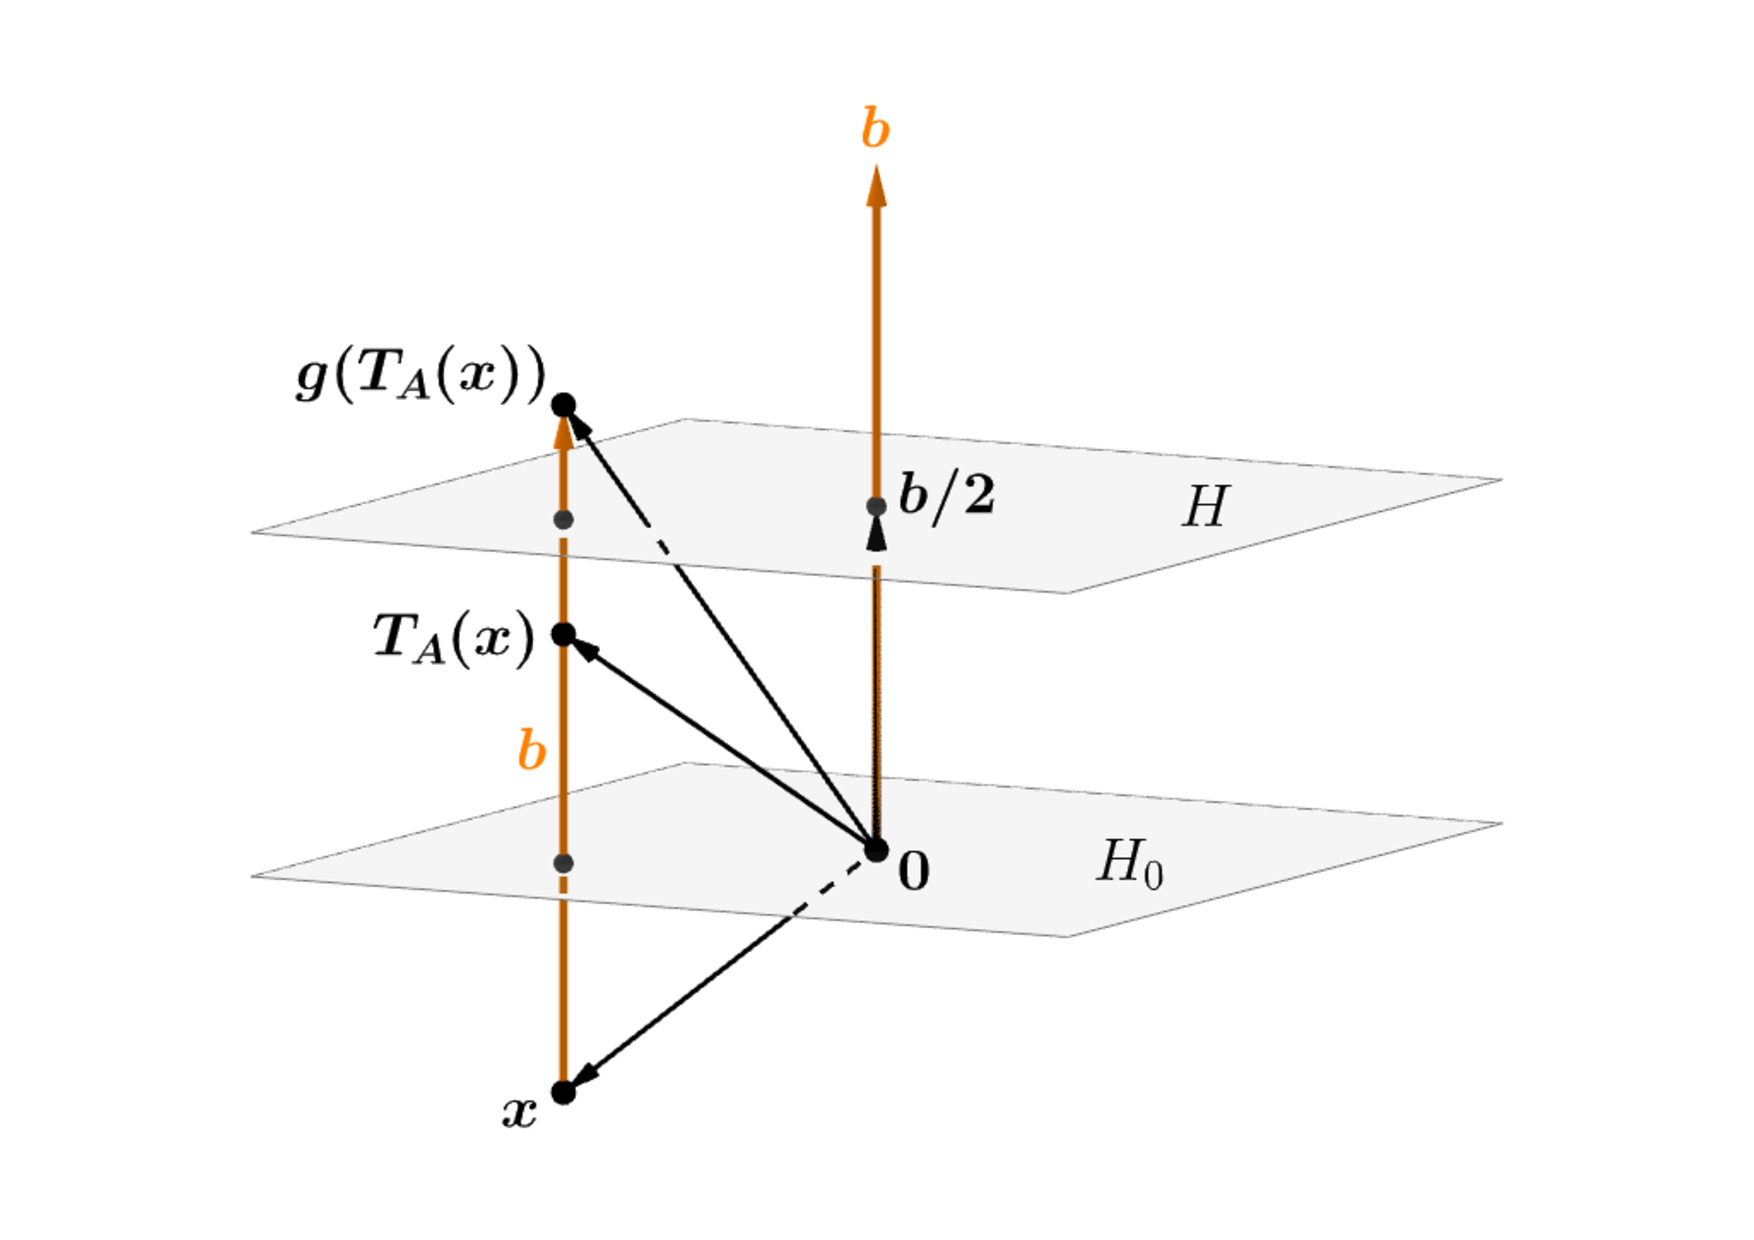
\includegraphics[height=4.5cm]{pictures/translation3.pdf}
    \caption{平行移動は平行な2平面に関する $2$ 個の鏡映の合成である.}
    \label{fig:translation3}
  \end{figure}

  \noindent
  (2) 逆に,平行な $2$ 平面 $H_1, H_2 \; (H_1 \neq H_2)$ に関する鏡
  映 $r_1, r_2$ に対して,その合成 $r_2 \circ r_1$ が平行移動であること
  を示す.$r_1(\bm{x})=A_1\bm{x}+\bm{b}_1, \; r_2(\bm{x}) =
  A_2\bm{x}+\bm{b}_2$ とすると,
  \[
    A_1 \sim R_0 \sim A_2, \quad \bm{b}_1 \in V_{A_1}(-1), \; \bm{b}_2 \in V_{A_2}(-1)
  \]
  である.$H_1$ と $H_2$ が平行なので $V_{A_1}(1) = V_{A_2}(1)$ であ
  る.$(\bm{p}_1, \bm{p}_2)$ を $V_{A_1}(1)$ の正規直交基底と
  し,$(\bm{p}_3)$ を
  $V_{A_1}(-1)=V_{A_1}(1)^{\perp} = V_{A_2}(1)^{\perp}=V_{A_2}(-1)$ の
  正規直交基底とする.必要なら $\bm{p}_1$ と $\bm{p}_2$ を入れ替えて,$P:=\left[
    \begin{array}{ccc}
      \bm{p}_1 & \bm{p}_2 & \bm{p}_3
    \end{array}
  \right] \in SO(3)$ とすると,$P^{-1}A_1 P = R_0 = P^{-1}A_2 P$ より $A_1=PR_0P^{-1}=A_2$
  である.従って,$A=A_1= A_2$ とおくと,$A^2= E, \; \bm{b}_1 \in V_{A}(-1)$ より
  \[
    r_2 \left( r_1 (\bm{x})\right) = A\left( A \bm{x}+\bm{b}_1\right) + \bm{b}_2
    = \bm{x} + A \bm{b}_1 + \bm{b}_2 = \bm{x} + \bm{b}_2 - \bm{b}_1
  \]
  だから $r_2 \circ r_1 = t_{\bm{b}_2-\bm{b}_1}$ である.すなわ
  ち,$r_2 \circ r_1$ は平行移動である.なお,$r_1 \neq r_2$ だか
  ら $\bm{b}_1 \neq \bm{b}_2$ より $t_{\bm{b}_2-\bm{b}_1}$ は恒等変換で
  はない.このとき,$\bm{b}_1, \bm{b}_2 \in V_{A}(-1)^{\perp}$ だか
  ら,$\bm{b}_2-\bm{b}_1$の向きは $H_1$ から $H_2$ の方へ両平面に直交す
  る方向である.さらに,図\ref{fig:translation3gen}のように $H_1, H_2$
  はそれぞれ $\bm{b}_1/2, \; \bm{b}_2/2$ を通り $V_{A}(1)$ に平行な平面
  だから,その距離は $\|\bm{b}_2-\bm{b}_1\|/2$ である.
  \begin{figure}[h]
    \centering
    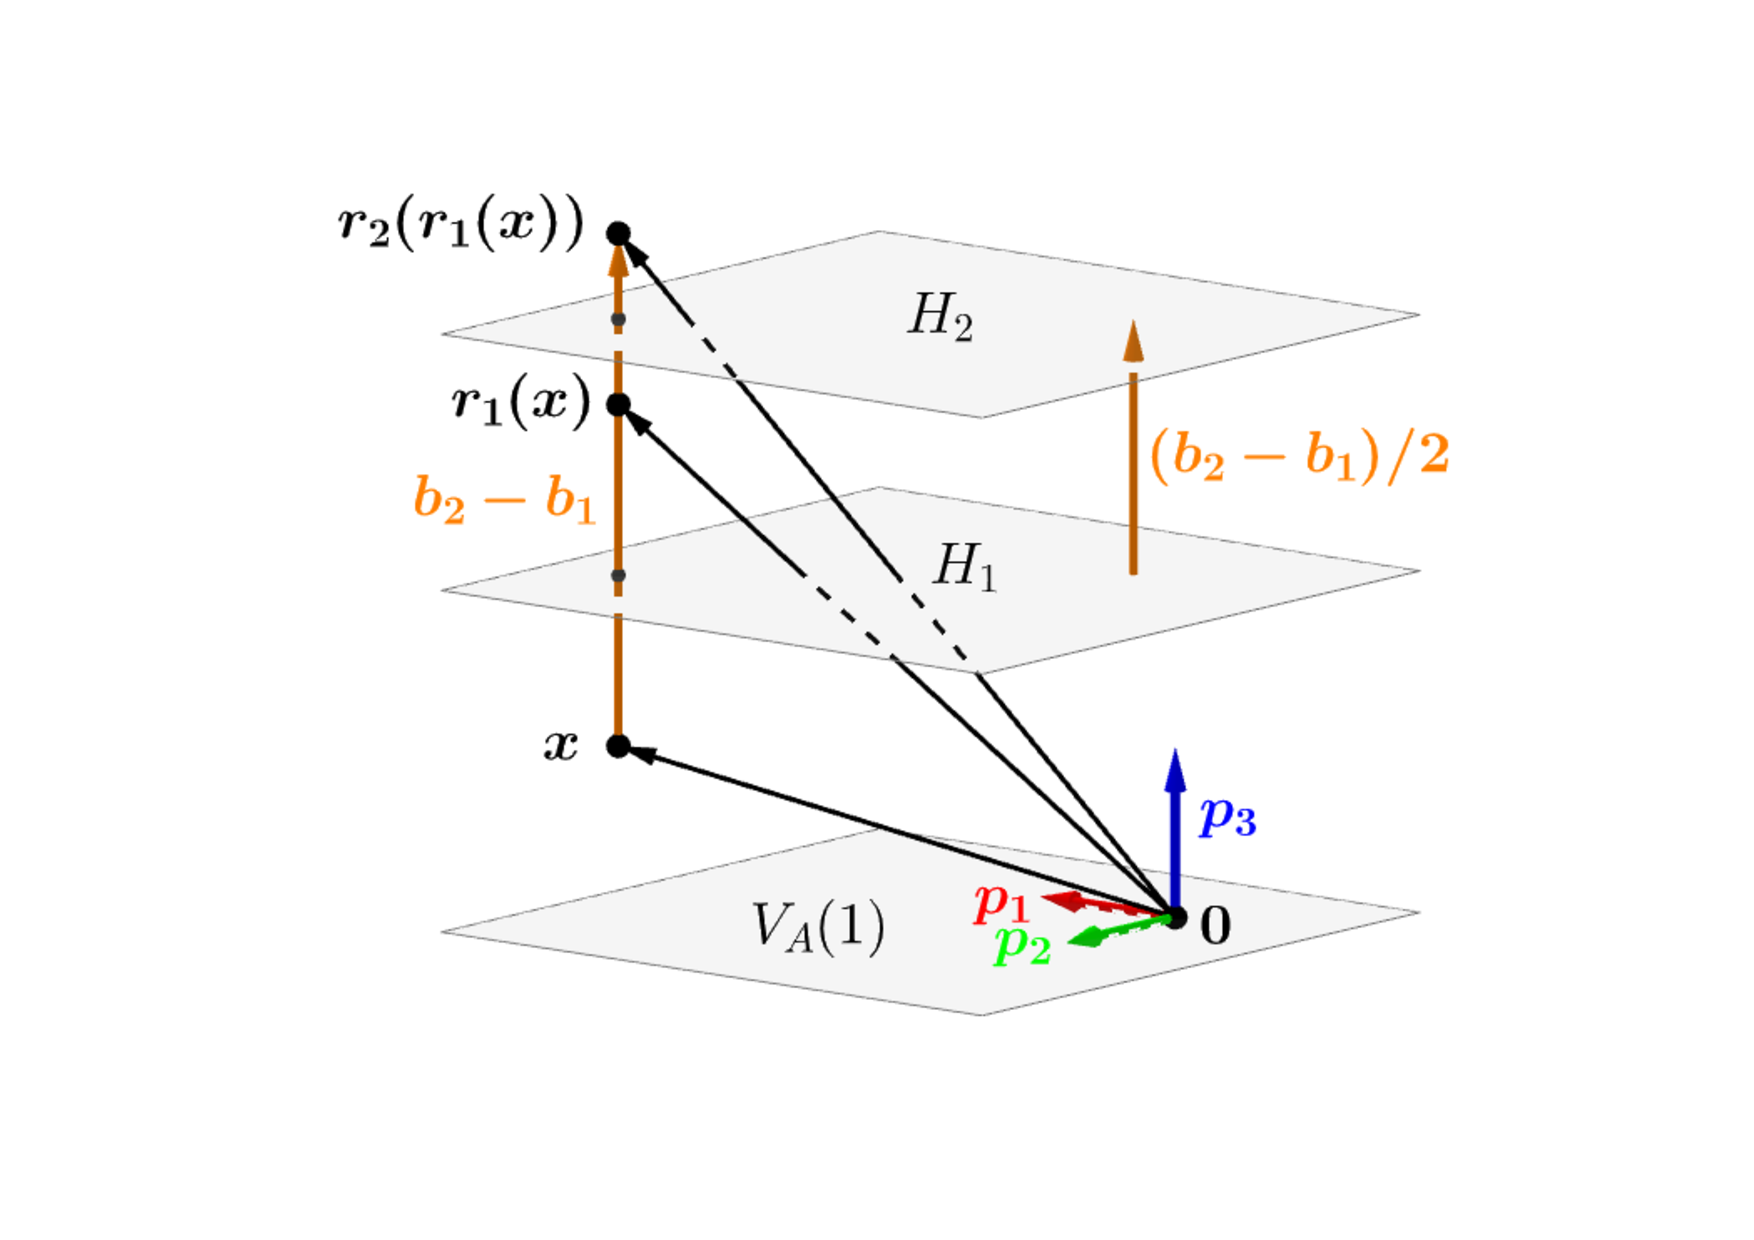
\includegraphics[height=4.5cm]{pictures/translation3gen.pdf}
    \caption{平行な $2$ 平面に関する $2$ 個の鏡映の合成は平行移動である.}
    \label{fig:translation3gen}
  \end{figure}
\end{proof}

\begin{lemma}\label{lem:rotation3}
  \begin{enumerate}[(1)]
  \item 空間 $\mathbb{R}^3$ の $\theta$ 回転 $f$ は鏡映面が平行でな
    い $2$ 個の鏡映の合成である.このとき,$2$ つの鏡映面の交線が $f$
    の回転軸であり,2つの鏡映面のなす角は $\theta/2$ である.
    
  \item 逆に,平行でない $2$ 平面 $H_1, H_2$ に
  関する鏡映を $g_1, g_2$ とすると,合成 $g_2 \circ g_1$ は $2$ 平面の
  交線を軸とする回転であり,回転方向は $H_1$ から $H_2$ へ,回転角
  は $2$ 平面の交わる角の $2$ 倍である.
  \end{enumerate}
\end{lemma}

\begin{proof}
  (1) 任意に $\bm{c} \in \Fix(f)$ をとる.$f$ は $A \sim S_{\theta}$ と
  なる直交行列 $A \in SO(3)$ によって
  \[
    f(\bm{x}) = A(\bm{x} - \bm{c}) + \bm{c}
  \]
  と書ける.$f$ の回転軸 $\Fix(f)$ は直線 $V_A(1)$ に平行である.そこ
  で,$f$ の回転の正の方向に回転する右ねじの進む方向の単位ベクトル
  を $\bm{p}_3$ とすと,$\bm{p}_3 \in V_A(1)$
  である.$\bm{p}_1, \bm{p}_2 \in V_A(1)^{\perp}$ を
  $(\bm{p}_1, \bm{p}_2, \bm{p}_3)$ が空間 $\mathbb{R}^3$ の右手系正規直
  交基底となるように選ぶ.このとき,
  \[
     S_{\theta} = {}^{t}PAP, \quad P := \left[
      \begin{array}{ccc}
        \bm{p}_1 & \bm{p}_2 & \bm{p}_3
      \end{array}
    \right]\in SO(3)
  \]
  である.$g_2$ を $\bm{c}+\bm{p}_1$ と $f(\bm{c}+\bm{p}_1)$ の垂直二等
  分面 $H_2$ に関する鏡映とし,$g_1 = g_2 \circ f$
  とする.$\Fix(f) \subset H_2 = \Fix(g_2)$ だから補
  題\ref{lem:inv-comp3}より
  \[
    \Fix(f) = \Fix(g_2) \cap \Fix(f) \subset \Fix(g_2 \circ f) = \Fix(g_1)
  \]
  である.さらに,$\bm{p}_1$ は $\Fix(f)$ に直交し,
  \[
    g_1 (\bm{c}+\bm{p}_1) = g_2 \left( f(\bm{c}+\bm{p}_1)\right) = \bm{c}+\bm{p}_1
  \]
  より $\bm{c}+\bm{p}_1 \in \Fix(g_1)$ であるか
  ら,$\Fix(g_1)$ は $\Fix(f)$ を含み $\bm{p}_1$ に平行な平面,すなわ
  ち,$\bm{c}$ を通り $\bm{p}_2$ に直交する平面 $H_1$ を含む.一方,
  図\ref{fig:cutplane3}から
  \[
    g_1(\bm{c} + \bm{p}_2) = g_2 \left( f(\bm{c}+\bm{p}_2) \right) = c-\bm{p}_2 \neq c+\bm{p}_2
  \]より $c+\bm{p}_2 \notin \Fix(g_1)$ である.従って,
  $\Fix(g_1) \neq \mathbb{R}^3$ であるから \ref{sec:inv3}節で見たよう
  に $\Fix(g_1)$ は平面 $H_1$ である.分類表\ref{tab:classification3}か
  ら,固定点集合が平面となるのは鏡映であるから $g_1$ は鏡映である.よって,
  \[
    f = (g_2 \circ g_2) \circ f = g_2 \circ (g_2 \circ f) = g_2 \circ g_1
  \]
  より,$f$ は $2$ 個の鏡映 $g_1, g_2$ の合成である.また,空
  間 $\mathbb{R}^3$ の中で$2$ 平面 $H_1, H_2$ が共に直線 $\Fix(f)$ を含
  むので,$H_1 \cap H_2 = \Fix(f)$ である.すなわち,$2$ 平面の交線
  が $f$ の回転軸である.さらに,図\ref{fig:cutplane3}のように $H_1,
  H_2$ のなす角は $\theta/2$ である.
  \begin{figure}[h]
    \centering
    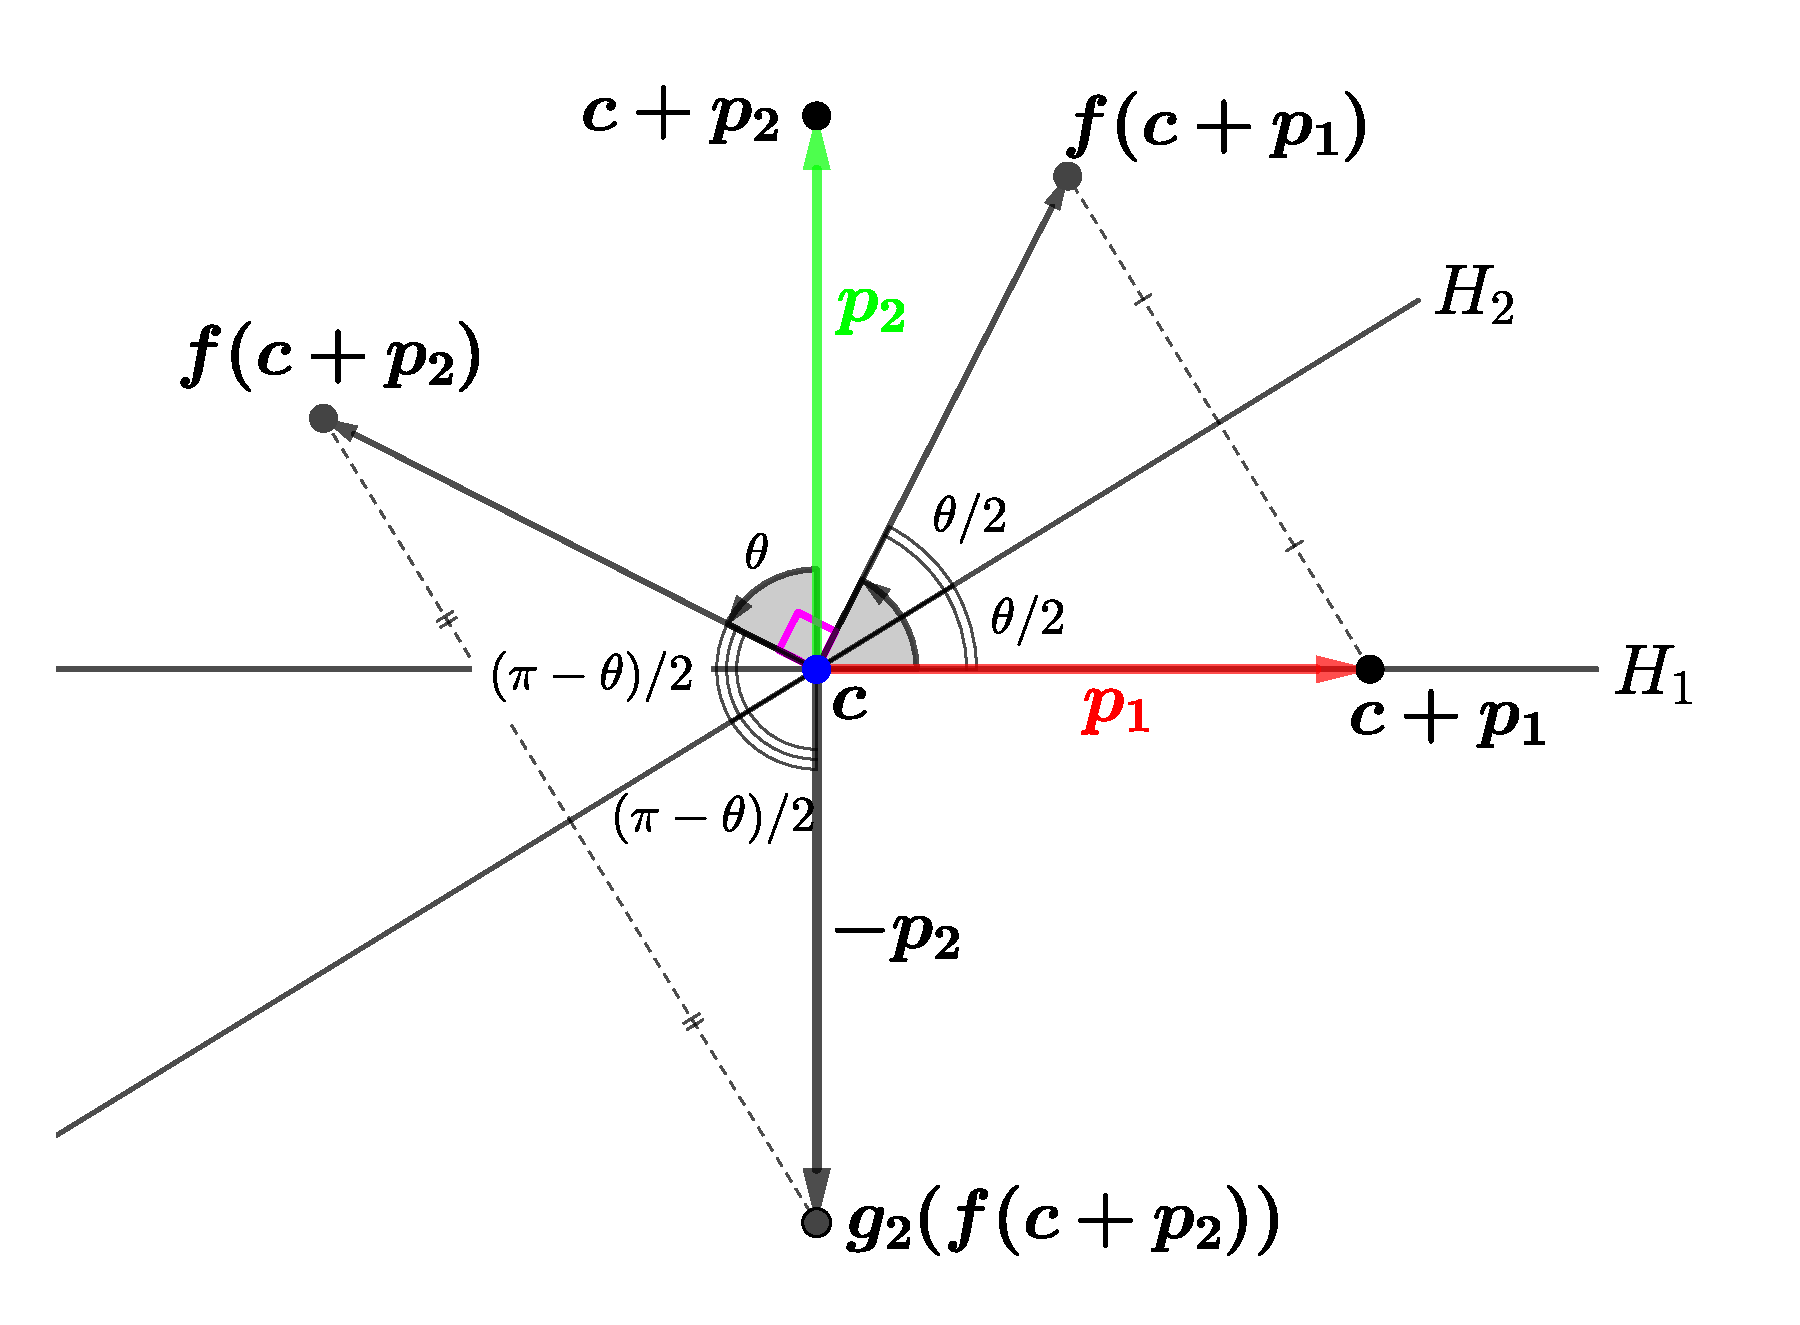
\includegraphics[height=4.5cm]{pictures/cutplane3.pdf}
    \caption{$g_1(\bm{c}+\bm{p}_2) = g_2\left( f(\bm{c}+\bm{p}_2)\right) = \bm{c}-\bm{p}_2$}\label{fig:cutplane3}
  \end{figure}

 
  
  % 以上の準備のもとで実
  % 際に証明に入る前に,証明の幾何学的な背景を説明しておこう.幾何学的
  % な感覚が十分に備わっているなら以下の枠内は読み飛ばしてもよい.
  
  % \begin{screen}
  %    $f=g_2 \circ g_2$ となる空間の鏡映 $g_1, g_2$ を見つけるために,
  %   そのような $g_1, g_2$ がどのようなものでなければならないかを考え
  %   よう.

  %    2つの鏡映面 $H_1:=\Fix(g_1)$ と $H_2:=\Fix(g_2)$ が平行なときは補
  %   題\ref{lem:translation3}から $g_2 \circ g_1$ は平行移動になってしま
  %   うので,$H_1, H_2$ は平行ではない.空間の中で平行でない $2$ 平面は
  %   必ず交わり,その交点全体 $H_1 \cap H_2$ は直線をなす.今 $f=g_2
  %   \circ g_1$ であって欲しいが,$\Fix(f)$ は直線なので補
  %   題\ref{lem:inv-comp3}から $H_1 \cap H_2 \subset \Fix(g_2 \circ
  %   g_1)$ より $H_1 \cap H_2 =\Fix(f)$ となる,すなわち,$2$ 平面の交線
  %   が回転の軸になるはずである.

  %    $2$ つの鏡映面のなす角を考えよう.下図のように,$f$ の回転
  %   軸 $\Fix(f)$ に $\bm{c} \in \Fix(f)$ で直交する平面 $H_0$ 上で $f$
  %   を見ると,$f$ は $c$ を中心とした平面 $H_0$ 上での $\theta$ 回転で
  %   ある.これは,平面 $H_0$ 上では直線 $H_1 \cap H_0$ に関する鏡映と直
  %   線 $H_2 \cap H_0$ に関する鏡映の合成である.従って,定
  %   理\ref{thm:generate2}で見たように $2$ 直線 $H_1 \cap H_0$ と $H_2
  %   \cap H_0$ のなす角は $\theta /2$ である.$2$ つの鏡映面 $H_1, H_2$
  %   は共に $H_0$ に直交するので,結局 $H_1, H_2$ のなす
  %   角は $\theta/2$ に等しいはずである.
  %   \begin{center}
  %     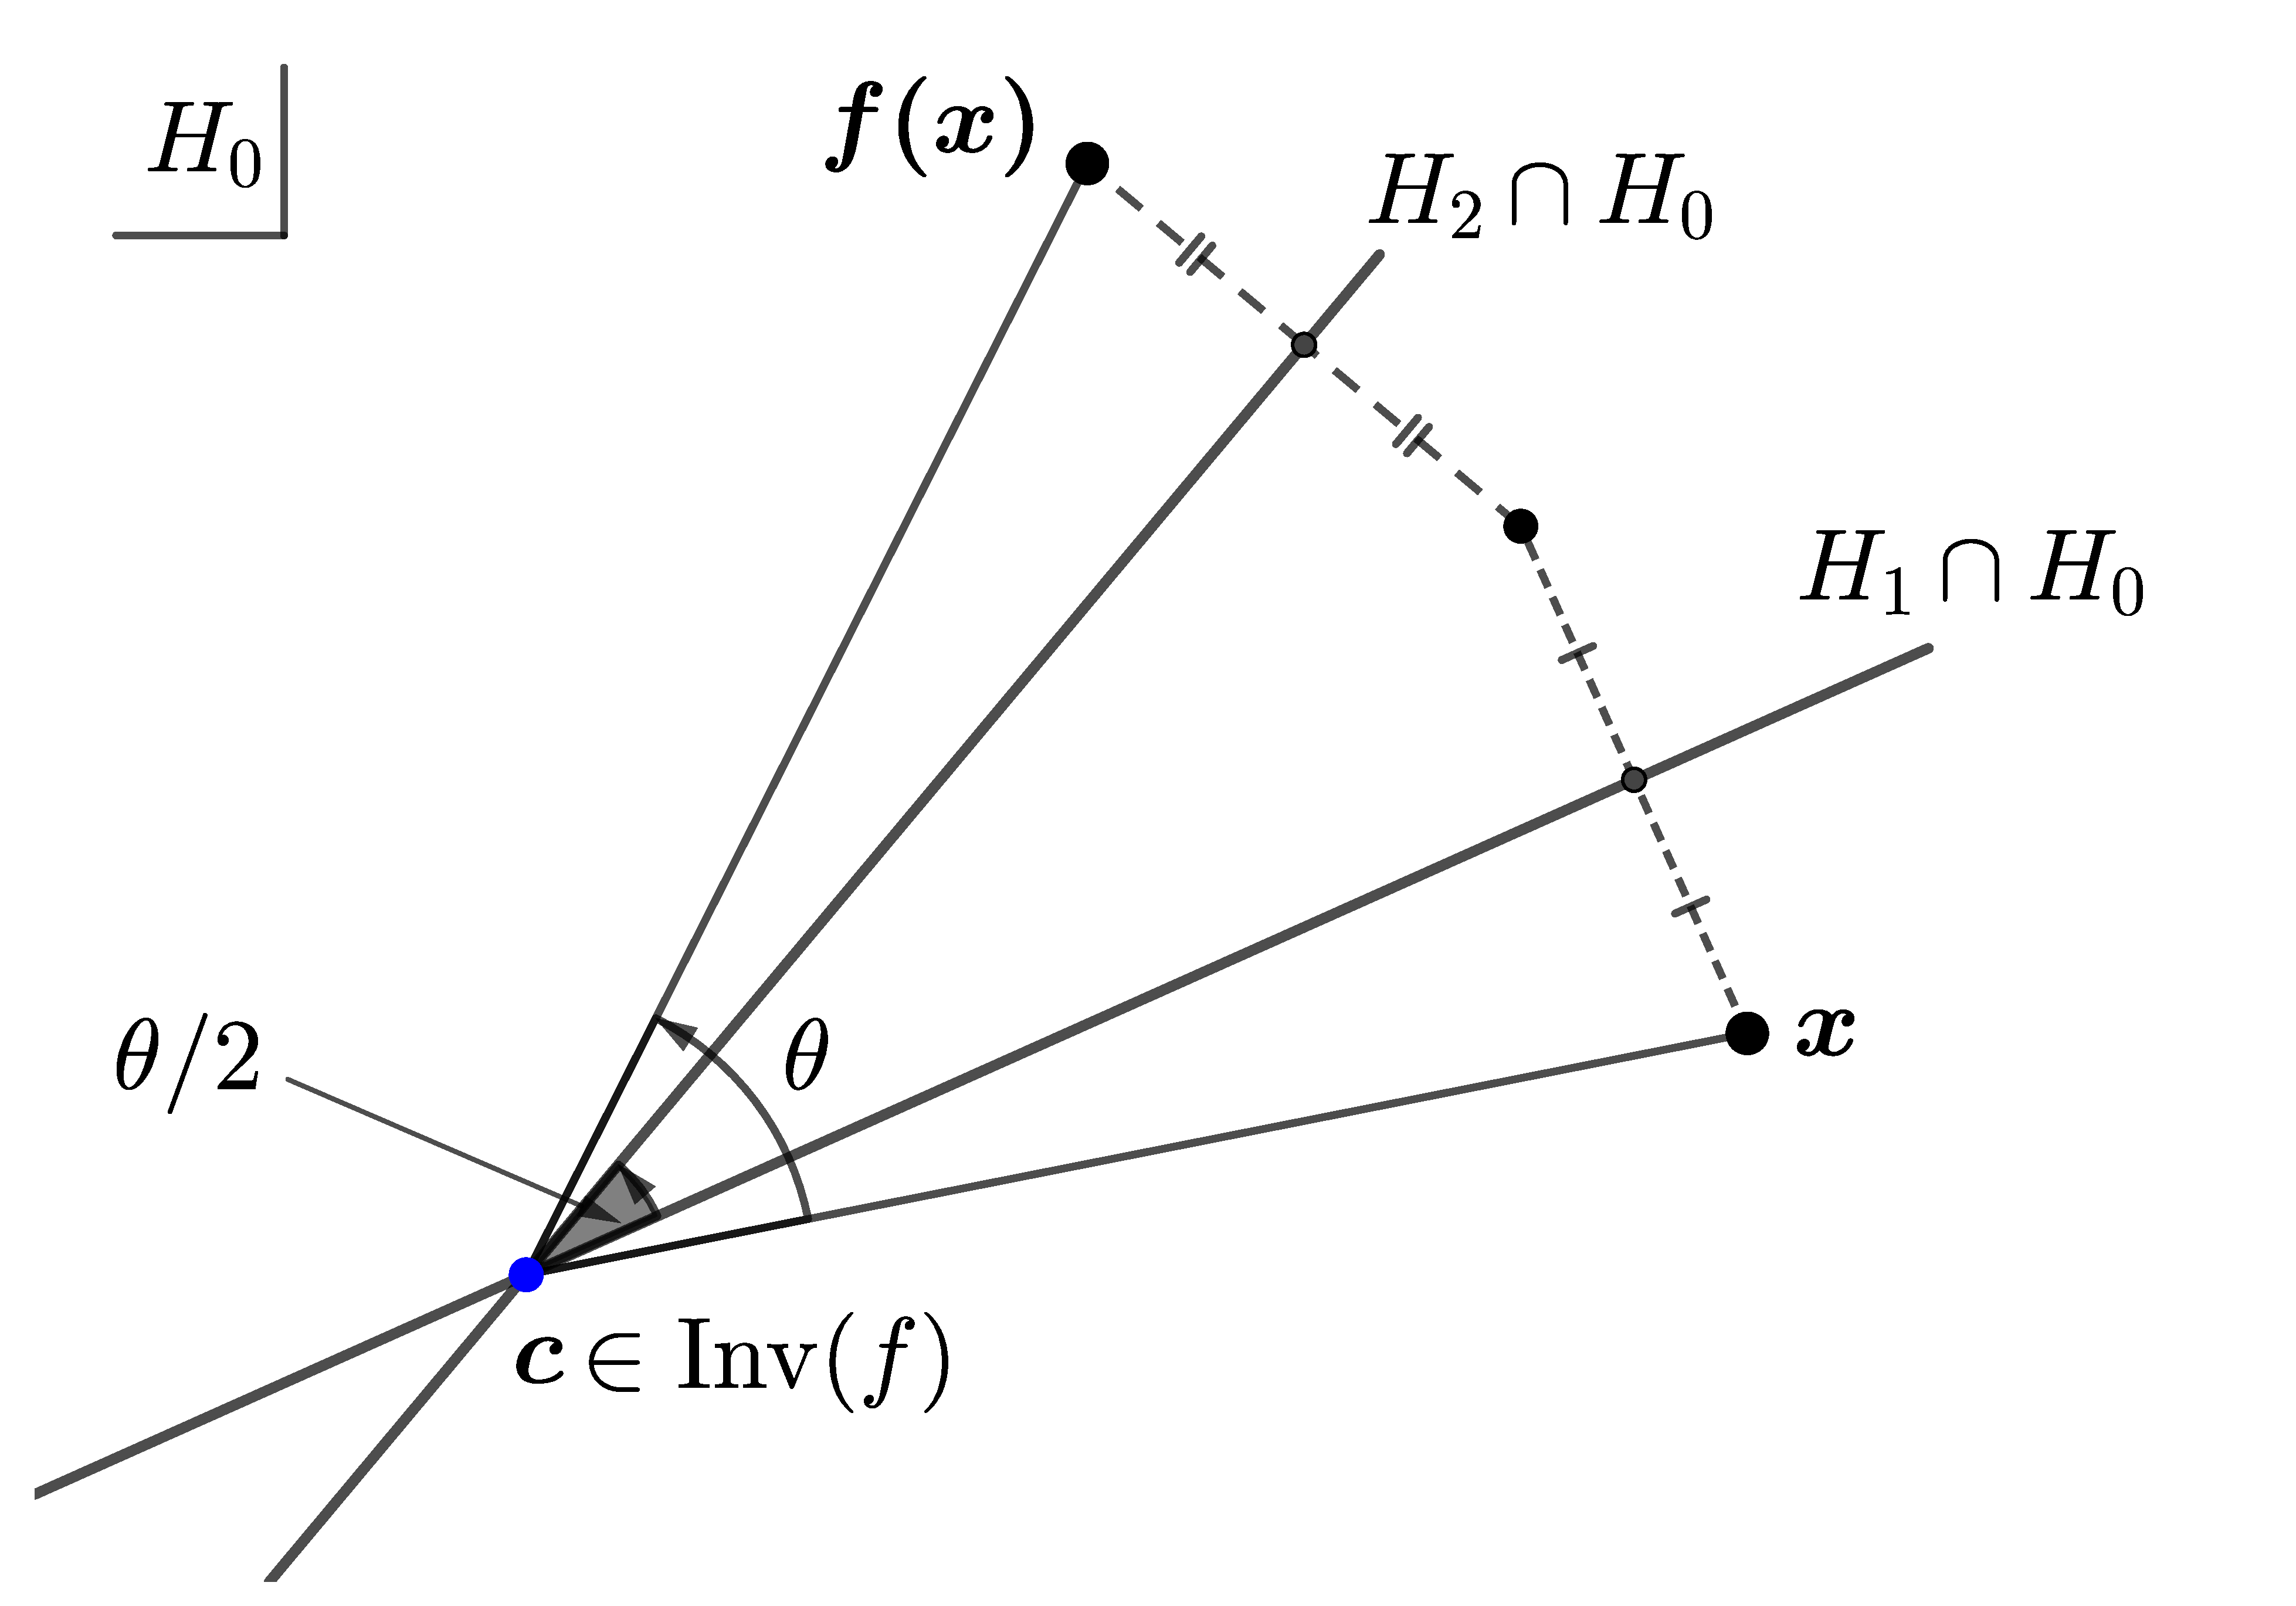
\includegraphics[height=5cm]{pictures/cut_rotation3.pdf}
  %   \end{center}
  % \end{screen}
  
  % \begin{screen}
  %    実際に $g_1, g_2$ を具体的に書き下そう.定
  %   理\ref{thm:RefOrGlide3}から,任意の $\bm{c} \in H_1 \cap
  %   H_2$ に対して
  %   \[
  %     g_1(\bm{x}) = B_1(\bm{x}-\bm{c}) + \bm{c}, \quad g_2(\bm{x}) = B_2 (\bm{x}-\bm{c})+\bm{c}
  %     \quad (B_1 \sim R_0 \sim B_2)
  %   \]
  %   と書ける.そして
  %   \[
  %     g_2(g_1(\bm{x})) = B_2 (B_1(\bm{x}-\bm{c})+\bm{c}-\bm{c})+\bm{c}= B_2 B_1(\bm{x}-\bm{c}) + \bm{c}
  %   \]
  %   である.これが $f(\bm{x})$ に等しくあって欲しいのだが,$\bm{c}
  %   \in \Fix(f)$ でもあるので,$f(\bm{x})$ は
  %   \[
  %     f(\bm{x})=A(\bm{x}-\bm{c})+\bm{c}
  %   \]
  %   とも書ける.従って,$f=g_2\circ g_1$ であるためには $A=B_2B_1$ となればよいことが分かる.
    
  %    直交行列 $B_1, B_2$ は共に $R_0$
  %   に標準化されるので,${}^{t}Q_1 B_1 Q_1 = {}^{t}Q_2 B_2 Q_2 = R_0$
  %   となる $Q_1, Q_2 \in SO(3)$ を見つけよう.まず,$Q_1 = \left[
  %       \begin{array}{ccc}
  %         \bm{q}_1 & \bm{q}_2 & \bm{q}_3
  %       \end{array}
  %     \right]$ とおいてみよう.このとき,
  %     \[
  %       V_{B_1}(1) = \langle \bm{q}_1, \bm{q}_2\rangle, \quad V_{B_1}(-1)=\langle \bm{q}_3\rangle
  %     \]
  %     である.$g_1$ の鏡映面 $H_1$ は $\bm{c}$ を通り $V_{B_1}(1)$ に平
  %     行な平面であり,これが $\bm{c}$ を通り $\bm{p}_3$ に平行な直
  %     線 $\Fix(f)$ を含むので,$\bm{p}_3 \in V_{B_1}(1)$ である.$H_1$
  %     と $H_2$ のなす角は $\theta/2$ であって欲しいが,このような $2$
  %     平面の選び方は無数にある.そこで,枠外の図\ref{fig:rotation3ref}の
  %     ように $H_1$ が $\bm{p}_2$ に直交するものを選ぼう.すなわち,
  %     \[
  %       V_{B_1}(1) = \langle \bm{p}_1, \bm{p}_3\rangle, \quad V_{B_1}(-1) = \langle \bm{p}_2\rangle
  %     \]
  %     としよう.さらに,$Q_1 \in SO(3)$ であって欲しいので,
  %     \[
  %       Q_1 =\left[
  %         \begin{array}{ccc}
  %           \bm{p}_3 & \bm{p}_1 & \bm{p}_2
  %         \end{array}
  %       \right]
  %     \]
  %     とすれば,${}^{t}Q_1 B_1Q_1 = R_0$ となるはずである.そし
  %     て,$H_2$ は $\Fix(f)$ を軸として $H_1$ を $\theta/2$ 回転させた
  %     平面のはずなので,$V_{B_2}(1), V_{B_2}(-1)$ はそれぞ
  %     れ $V_{B_1}(1), V_{B_1}(-1)$ を $\bm{p}_3$ を軸として $\theta/2$
  %     回転させた平面と直線である.$C=PS_{\theta/2}{}^{t}P$ とする
  %     と,$\mathbb{R}^3$ の直交変換 $T_C(\bm{x}) =
  %     C\bm{x}$ は $\bm{p}_3$ を軸とする $\theta/2$ 回転であるから,
  %     \[
  %       V_{B_2}(1) = \langle T_C(\bm{p}_3), T_C(\bm{p}_1) \rangle,
  %       \quad V_{B_2}(-1) = \langle T_C(\bm{p}_2) \rangle
  %     \]
  %     である.$C \in SO(3)$ だから
  %     \[
  %       Q_2 = \left[
  %         \begin{array}{ccc}
  %           T_C(\bm{p}_3) & T_C(\bm{p}_1) & T_C(\bm{p}_2)
  %         \end{array}
  %       \right]
  %     \]
  %     とすれば $Q_2 \in SO(3)$ で,${}^{t}Q_2 B_2 Q_2 = R_0$ となるはずである.

  %      以上の幾何学的考察から,$B_1 = Q_1 R_0 {}^{t} Q_1$ と
  %     $B_2=Q_2 R_0 {}^{t}Q_2$ が $B_2 B_1=A$ を満たすはずであるから,あ
  %     とはこれを実際に計算によって確認すればよい.
  %   \end{screen}



  % $C=PS_{\theta/2}{}^{t}P$ とおく.直交変
  % 換 $T_C(\bm{x})=C\bm{x}$ は $\bm{p}_3$ を回転軸とする $\theta/2$ 回
  % 転である.
  % \[
  %   Q_1 = \left[
  %     \begin{array}{ccc}
  %       \bm{p}_3 & \bm{p}_1 & \bm{p}_2
  %     \end{array}
  %   \right], \quad 
  %   Q_2 =\left[
  %     \begin{array}{ccc}
  %       T_C(\bm{p}_3) & T_C(\bm{p}_1) & T_C(\bm{p}_2)
  %     \end{array}
  %   \right]
  % \]
  % とし,$B_1 = Q_1 R_0 {}^{t}Q_1, \; B_2=Q_2 R_0 {}^{t}Q_2$ とす
  % る.任意に $\bm{c} \in \Fix(f)$ をと
  % り
  % \[
  %   g_1(\bm{x}) = B_1(x-\bm{c})+\bm{c}, \quad g_2(\bm{x})=B_2(\bm{x}-\bm{c})+\bm{c}
  % \]
  % とすると,$Q_1, Q_2 \in SO(3)$ なので,$B_1 \sim R_0 \sim
  % B_1$ より $g_1, g_2$ はそれぞれ平面 $H_1:=\Fix(g_1)$ と平面 $
  % H_2:=\Fix(g_2)$ に関する鏡映である.ここで,$P$ は直交行列だから
  % \begin{align*}
  %   Q_1 &=PT, \quad T:= \left[
  %   \begin{array}{ccc}
  %     0 & 1 & 0\\
  %     0 & 0 & 1\\
  %     1 & 0 & 0
  %   \end{array}
  %             \right],\\
  %   Q_2 &= \left[
  %         \begin{array}{ccc}
  %           C\bm{p}_3 & C\bm{p}_1 & C\bm{p}_2
  %         \end{array}
  %                                  \right] =  CQ_1 = CPT = PS_{\theta/2}{}^{t}PPT = PS_{\theta/2}T
  % \end{align*}
  % と書ける.これと $R_0, P, T \in O(3)$ から
  % \begin{align*}
  %   B_2 B_1 &= Q_2 R_0 {}^{t}Q_2 Q_1 R_0 {}^{t}Q_1
  %             =PS_{\theta/2}TR_0\ {}^{t}\left(PS_{\theta/2}T\right)PT R_0\ {}^{t}\left(PT\right)\\
  %           &=PS_{\theta/2}\left(TR_0 {}^{t}T\right) {}^{t}S_{\theta/2} 
  %             \left({}^{t}P P\right)\left(TR_0 {}^{t}T\right){}^{t}P
  %             =PS_{\theta/2}\left(TR_0{}^{t}T\right)\left({}^{t}S_{\theta/2}TR_0{}^{t}T\right){}^{t}P\\
  %           &=P S_{\theta/2}\left(TR_0{}^{t}T\right) \ {}^{t}\left( T \ {}^{t}R_0 {}^{t} T S_{\theta/2}\right) {}^{t}P 
  %             = PS_{\theta/2}{}^{t}\left( \left({}^{t}S_{\theta/2} T R_0 {}^{t} T\right) 
  %             \left( T \ {}^{t}R_0 {}^{t}T\right)\right) {}^{t}P\\
  %           &=PS_{\theta/2}  S_{\theta/2}\ {}^{t}P = P S_{\theta} {}^{t}P = A
  % \end{align*}
  %   である.従って,
  % \[
  %   g_2 \left( g_1(\bm{x})\right) = B_2\left( B_1(\bm{x}-\bm{c}) + \bm{c} - \bm{c}\right) + \bm{c}
  %   = B_2 B_1 (\bm{x}-\bm{c})+\bm{c} = A(\bm{x}-\bm{c}) + \bm{c} = f(\bm{x})
  % \]
  % より,$f=g_2 \circ g_1$ である.また,鏡映面 $H_1$ は $\bm{c}$ を通
  % り $V_{B_1}(1)$ に平行な平面であり,$H_2$ は $\bm{c}$ を通
  % り $V_{B_2}(1)$ を通る平面である.
  % \[
  %   T_C(\bm{p}_3) = C \bm{p}_3 = PS_{\theta/2}{}^{t}P \bm{p}_3 = PS_{\theta/2}\left(\left[
  %     \begin{array}{c}
  %       {}^{t}\bm{p}_1\\
  %       {}^{t}\bm{p}_2\\
  %       {}^{t}\bm{p}_3
  %     \end{array}
  %   \right] \bm{p}_3 \right)= P\left(S_{\theta/2} \bm{e}_3\right) = P
  % \bm{e}_3 = \bm{p}_3
  % \]
  % なので,$Q_1, Q_2$ の定義から
  % \[
  %   V_{B_1}(1) = \langle \bm{p}_3, \bm{p}_1\rangle, \quad V_{B_2}(1) =
  %   \langle T_C(\bm{p}_3), T_C(\bm{p}_1)\rangle = \langle \bm{p}_3, T_C(\bm{p}_1)\rangle
  % \]
  % より,$H_1, H_2$ は $\bm{c}$ を通り $\bm{p}_3$ に平行な直線,すなわ
  % ち,$\Fix(f)$ を含む.空間の中で平面と平面の交わりは直線なの
  % で,$\Fix(f) = H_1 \cap H_2$ である.よって,
  % 図\ref{fig:rotation3ref}のように $H_1$ を直線 $\Fix(f)$ を軸とし
  % て $\theta/2$ 回転させた平面が $H_2$ である.つまり,$H_1$ と $H_2$
  % のなす角は $\theta/2$ である.

  \noindent
  (2) 逆に,平行でない任意の $2$ 平面 $H_1, H_2$ に関する鏡映 $g_1,
  g_2$ に対して,その合成 $g_2 \circ g_1$ が回転であることを示す.(1)で
  定義した記号は一旦全てリセットする.(1)では $A$ から $B_1, B_2$ を構
  成したが,今度は逆に $B_1, B_2$ から $A$ を構成していく.

  $2$ 平面 $H_1, H_2$ の交線を $L$ とする.すなわち,$L=H_1 \cap H_2$
  である.任意に $\bm{c} \in L$ をとる.$g_1, g_2$ はそれぞれ $H_1,
  H_2$ に関する鏡映なので,$B_1 \sim R_0 \sim B_2$ となる $B_1 , B_2
  \in O(3)$ によって
  \[
    g_1(\bm{x}) = B_1 (\bm{x}-\bm{c})+\bm{c}, \quad g_2(\bm{x}) =
    B_2(\bm{x}-\bm{c})+\bm{c}
  \]
  と書ける.$2$ 平面 $H_1, H_2$ の交わる角を $\theta/2$ とする.すなわ
  ち,交わる角の $2$ 倍を $\theta$ とする.
  \[
    g_2 ( g_1(\bm{x})) = B_2\left(B_1(\bm{x}-\bm{c})+\bm{c} - \bm{c}\right) + \bm{c} 
    = B_2 B_1(\bm{x}-\bm{c})+\bm{c}
  \]
  であるから,$A:=B_2 B_1 \sim S_{\theta}$ となることを示せばよい.

  
  直線 $L$ の単位方向ベクトルを $\bm{p}_3$ とする.すなわ
  ち,$\|\bm{p}_3\|=1$
  かつ$L=\Set{\bm{c} + t \bm{p}_3 | t \in \mathbb{R}}$ である.ただ
  し,$\bm{p}_3$ の向きは $H_1$ から $H_2$ の方向へ回転する右ねじの進む
  方向と同じとする.図\ref{fig:rotation3ref}のよう
  に $\bm{p}_2$ を $H_1$ に直交する単位ベクトルとし,$(\bm{p}_3,
  \bm{p}_1, \bm{p}_2)$ が $\mathbb{R}^3$ の右手系正規直交基底となるよう
  に $\bm{p}_1 \in V_{B_1}(1)$ をとる.具体的には $\mathbb{R}^3$ の外積
  を用いて $\bm{p}_1 = \bm{p}_2 \times \bm{p}_3$ とすればよい.
  \begin{figure}[h]
    \centering
    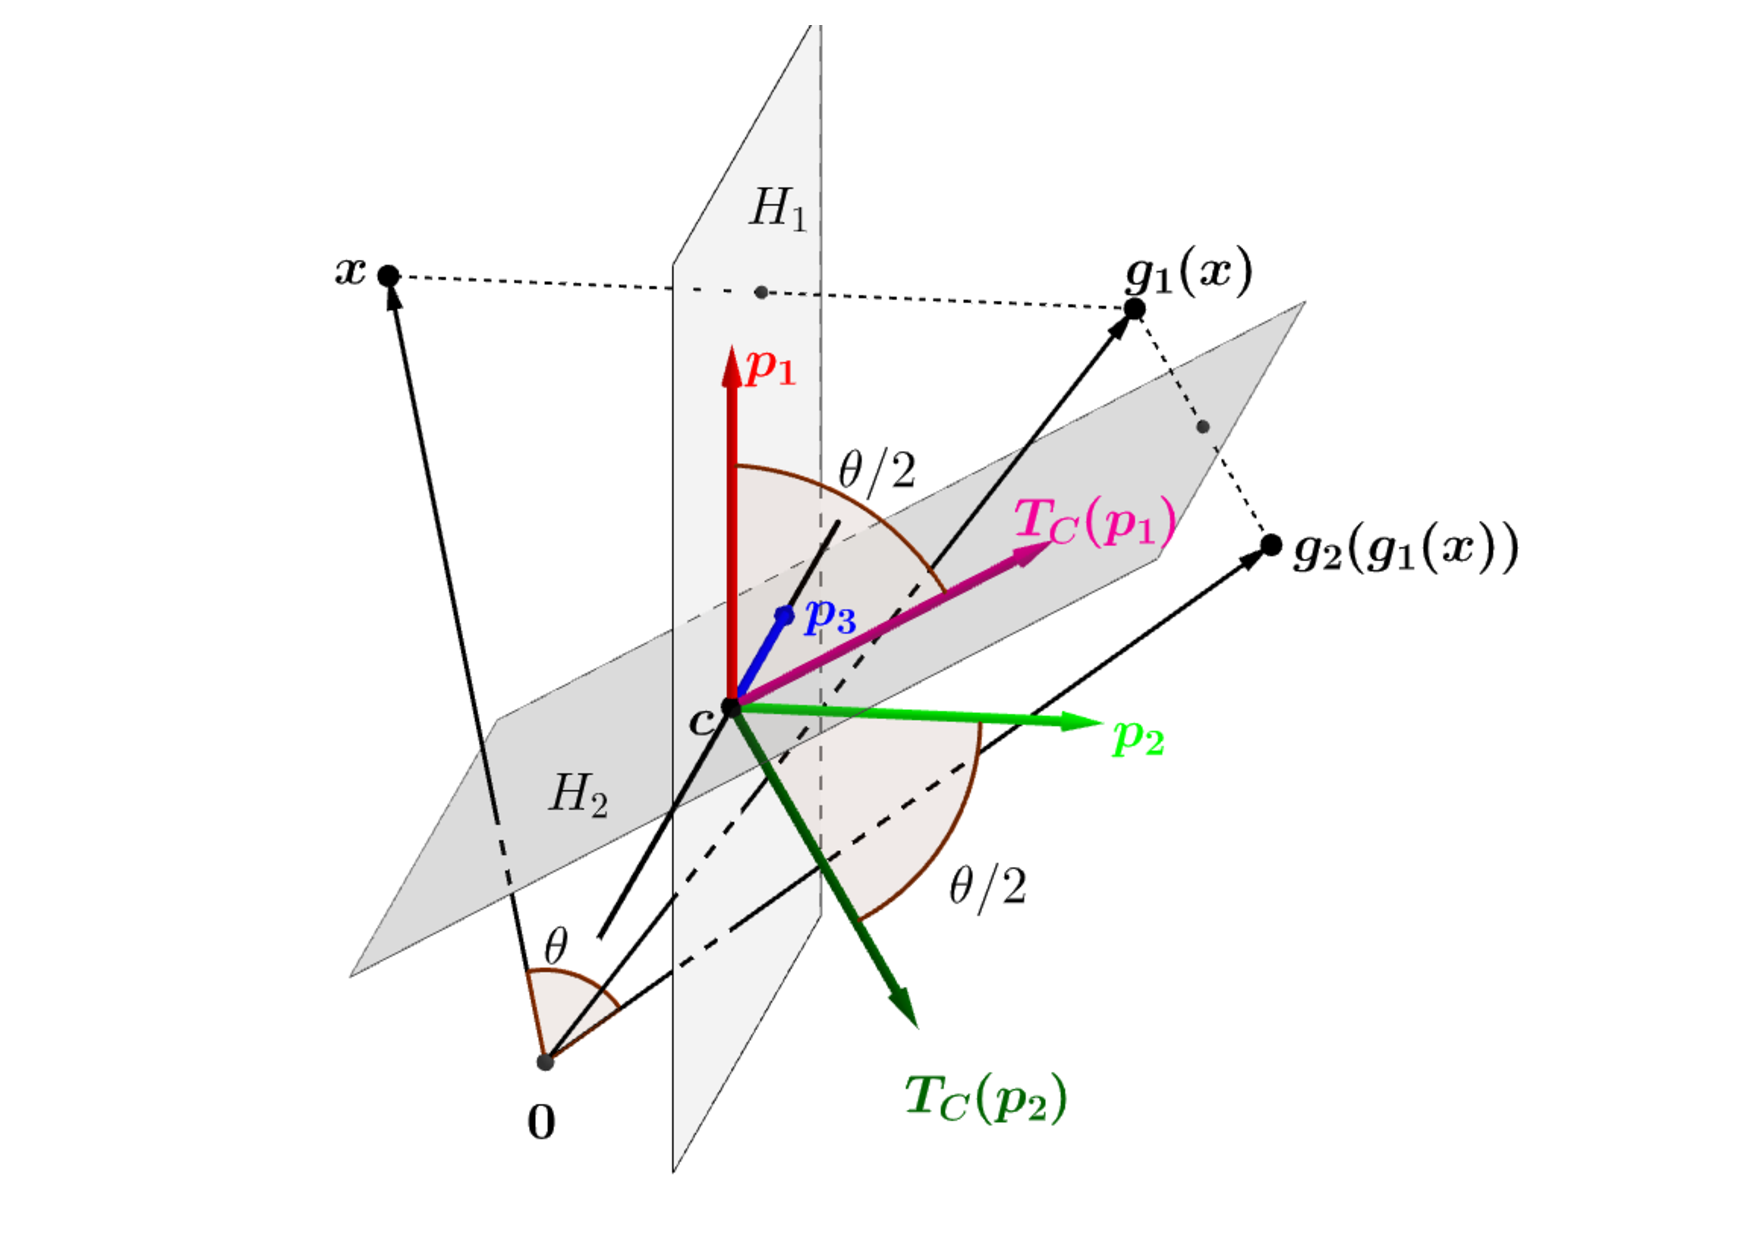
\includegraphics[height=4.5cm]{pictures/rotation3ref.pdf}
    \caption{平行でない $2$ 平面に関する $2$ 個の鏡映の合成は回転である.}
    \label{fig:rotation3ref}
  \end{figure}

  \noindent
  $H_1$ は $V_{B_1}(1)$
  に平行だから,$V_{B_1}(1) = \langle \bm{p}_3, \bm{p}_1\rangle, \;
  V_{B_1}(-1) = V_{B_1}(1)^{\perp}= \langle \bm{p}_2\rangle$ より
  \[
    {}^{t} Q_1 B_1 Q_1 = R_0, \quad Q_1:=\left[
      \begin{array}{ccc}
        \bm{p}_3 & \bm{p}_1 & \bm{p}_2
      \end{array}
    \right] \in SO(3)
  \]
  である.また,$(\bm{p}_1, \bm{p}_2, \bm{p}_3)$ は $\mathbb{R}^3$ の右
  手系正規直交基底なので
  \[
    P=\left[
      \begin{array}{ccc}
        \bm{p}_1 & \bm{p}_2 & \bm{p}_3
      \end{array}
    \right] , \quad C=P S_{\theta/2} {}^{t}P
  \]
  とすると,$P \in SO(3)$ であり,直交変換 $T_C(\bm{x}) =
  C\bm{x}$ は $\bm{p}_3$ を軸とする $\theta/2$ 回転である.ただし,回転
  の方向は $\bm{p}_3$ の向きに進む右ねじの回転方向,すなわち,$H_1$ か
  ら $H_2$ への方向である.平面 $H_1, H_2$ はそれぞれ $V_{B_1}(1),
  V_{B_2}(1)$ に平行で,$H_2$ は $L$ を軸に $H_1$ を $\theta/2$ 回転さ
  せた平面なので,$V_{B_2}(1) = \langle T_C(\bm{p}_3),
  T_C(\bm{p}_1)\rangle, \; V_{B_2}(-1)=V_{B_2}(1)^{\perp}=\langle
  T_C(\bm{p}_2)\rangle$ である.これより
  \[
    {}^{t}Q_2 B_2 Q_2 = R_0, \quad Q_2 :=\left[
      \begin{array}{ccc}
        T_C(\bm{p}_3) & T_C(\bm{p}_1) & T_C(\bm{p}_2)
      \end{array}
    \right] \in SO(3)
  \]
  である.ここで,$P$ は直交行列だから
  \begin{align*}
    Q_1 &=PT, \quad T:= \left[
    \begin{array}{ccc}
      0 & 1 & 0\\
      0 & 0 & 1\\
      1 & 0 & 0
    \end{array}
              \right],\\
    Q_2 &= \left[
          \begin{array}{ccc}
            C\bm{p}_3 & C\bm{p}_1 & C\bm{p}_2
          \end{array}
                                   \right] =  CQ_1 = CPT = PS_{\theta/2}{}^{t}PPT = PS_{\theta/2}T
  \end{align*}
  と書ける.これと $R_0, P, T \in O(3)$ から
  \begin{align*}
    B_2 B_1 &= Q_2 R_0 {}^{t}Q_2 Q_1 R_0 {}^{t}Q_1
              =PS_{\theta/2}TR_0\ {}^{t}\left(PS_{\theta/2}T\right)PT R_0\ {}^{t}\left(PT\right)\\
            &=PS_{\theta/2}\left(TR_0 {}^{t}T\right) {}^{t}S_{\theta/2} 
              \left({}^{t}P P\right)\left(TR_0 {}^{t}T\right){}^{t}P\\
            & =PS_{\theta/2}\left(TR_0{}^{t}T\right)\left({}^{t}S_{\theta/2}TR_0{}^{t}T\right){}^{t}P\\
            &=P S_{\theta/2}\left(TR_0{}^{t}T\right) \ {}^{t}\left( T \ {}^{t}R_0 {}^{t} T S_{\theta/2}\right) {}^{t}P \\
            &= PS_{\theta/2}{}^{t}\left( \left({}^{t}S_{\theta/2} T R_0 {}^{t} T\right) 
              \left( T \ {}^{t}R_0 {}^{t}T\right)\right) {}^{t}P\\
            &=PS_{\theta/2}  S_{\theta/2}\ {}^{t}P = P S_{\theta} {}^{t}P = A
  \end{align*}
    である.従って,
  \[
    g_2 \left( g_1(\bm{x})\right) = B_2\left( B_1(\bm{x}-\bm{c}) + \bm{c} - \bm{c}\right) + \bm{c}
    = B_2 B_1 (\bm{x}-\bm{c})+\bm{c} = A(\bm{x}-\bm{c}) + \bm{c} = f(\bm{x})
  \]
  より,$f=g_2 \circ g_1$ である.よって,$g_2 \circ
  g_1$ は $H_1$ と $H_2$ の交線 $L$ を軸とする $\theta$ 回転であり,回
  転方向は $T_C$ と同じ,すなわち,$H_1$ から $H_2$ への方向である.
 \end{proof}


 \begin{lemma}\label{lem:glide3}
   空間 $\mathbb{R}^3$ の滑り鏡映は $3$ 平面に関する$3$ 個の鏡映の
   合成として表すことができる.このとき,$3$ 平面の内 $2$ つは互いに平
   行で,共に残りの $1$ つと直交するものを選べる.また,$\mathbb{R}^3$
   の滑り鏡映を $2$ 個以下の鏡映の合成として表すことはできない.
 \end{lemma}

 \begin{proof}
   $f$ を空間 $\mathbb{R}^3$
   の滑り鏡映とする.$f(\bm{x}) = A\bm{x} + \bm{b} \; \left(A \sim
     R_0, \; \bm{b} \notin V_A(-1)\right)$ と書ける.
   \[
     \bm{b} = \bm{b}^{+} + \bm{b}^{-}, \quad \bm{b}^{+} \in V_A(1),
     \quad \bm{b}^{-} \in V_A(-1), \quad \bm{b}^{+} \neq \bm{0}
   \]
   とし,$r(\bm{x}) = A\bm{x} + \bm{b}^{-}$ とす
   る.$r$ は $\bm{b}^{-}/2$ を通り $\bm{b}^{-}$ に直交する平面 $H$ に
   関する鏡映である.
   \[
     f(\bm{x}) = \left(A\bm{x}+\bm{b}^{-}\right) + \bm{b}^{+} =
     t_{\bm{b}^{+}} \left( r(\bm{x})\right)
   \]
   より,$f=t_{\bm{b}^{+}} \circ r$ である.補
   題\ref{lem:translation3}より平行移
   動 $t_{\bm{b}^+}$ は $\bm{b}^{+}$ に直交する $2$ 平面 $H_1, H_2$
   に関する鏡映 $r_1, r_2$ の合成として $t_{\bm{b}^{+}} = r_2 \circ
   r_1$ と表せるので,
   \[
     f = t_{\bm{b}^{+}} \circ r = r_2 \circ r_1 \circ r
   \]
   より $f$ は $3$ 個の鏡映の合成として表せる.このとき,$H_1, H_2$ は
   いずれも $\bm{b}^{+}$ に直交するので,互いに平行で,共に $H$ に直交
   する.
   
   また,補
   題\ref{lem:translation3}(2)補題\ref{lem:rotation3}(2)から $2$ 個の鏡
   映の合成は恒等変換か平行移動か回転なので,滑り鏡映を $2$ 個以下の鏡
   映の合成として表すことはできない.
 \end{proof}

\begin{lemma}\label{lem:rotref3}
  空間 $\mathbb{R}^3$ の回転鏡映は $1$ 点で交わる $3$ 平面に関する $3$
  個の鏡映の合成として表すことができる.また,$\mathbb{R}^3$ の回転鏡映
  を $2$ 個以下の鏡映の合成として表すことはできない.
\end{lemma}

\begin{proof}
  $f$ を空間 $\mathbb{R}^3$
  の回転鏡映とする.$f(\bm{x}) = A\bm{x} + \bm{b} \; \left( A \sim
    R_{\theta} \neq R_0 \right)$ と書ける.直交行列 $A$ が $P \in
  SO(3)$ によって $R_{\theta} = P^{-1} A P$ と標準化される とする.定
  理\ref{thm:rotref3}の証明と同様に,
  \begin{align*}
    &B=PS_{\theta}P^{-1}, \quad C=PR_{0}P^{-1}, \quad 
    \bm{b} = \bm{b}_1 + \bm{b}_2, \quad \bm{b}_1 \in V_A(-1), \; \bm{b}_2 \in V_A(-1)^{\perp}\\
    &g(\bm{x})=B\bm{x} + \bm{b}_2, \quad h(\bm{x})=C\bm{x}+\bm{b}_1
  \end{align*}
  とすると $f = g \circ h$ である.このとき,$g$ は $f$ の固定
  点 $\bm{c}$ を通り $V_A(-1)$ に平行な直線 $\Fix(g)$ を軸とす
  る $\theta$ 回転で,$h$ は $\bm{c}$ を通り $V_A(-1)^{\perp}$ に平行な
  平面 $H:=\Fix(h)$ に関する鏡映である.補題\ref{lem:rotation3}より回
  転 $g$ は $\Fix(g)$ を交線とする平面 $H_1, H_2$ に関する鏡映 $r_1,
  r_2$ により $g=r_2 \circ r_1$ と書ける.よって,
  \[
    f = g \circ h = r_2 \circ r_1 \circ h
  \]
  より $f$ は $3$ 個の鏡映の合成として表せる.また,補
  題\ref{lem:inv-comp3}から $H_1 \cap H_2 \cap H = \Fix(f)=\{\bm{c}\}$
  より $3$ つの鏡映面は $1$ 点 $\bm{c}$ で交わる.
  
  また,補
  題\ref{lem:translation3}(2)補題\ref{lem:rotation3}(2)から $2$ 個の鏡
  映の合成は恒等変換か平行移動か回転なので,回転鏡映を $2$ 個以下の鏡映
  の合成として表すことはできない.
\end{proof}

\begin{lemma}\label{lem:spiral3}
  空間 $\mathbb{R}^3$ の螺旋運動は $4$ 個の鏡映の合成として表せる.ま
  た,$\mathbb{R}^3$ の螺旋運動を $3$ 個以下の鏡映の合成として表すこと
  はできない.
\end{lemma}

\begin{proof}
  螺旋運動は平行移動と回転の合成である.補題\ref{lem:translation3}と補
  題\ref{lem:rotation3}より平行移動と回転はそれぞれ $2$ 個の鏡映の合成
  として表せるので,螺旋運動は $4$ 個の鏡映の合成として表せる.

  また,補題\ref{lem:translation3}と補題\ref{lem:rotation3}から螺旋運動
  を $2$ 個以下の鏡映の合成として表すことはできない.最後に,螺旋運動
  が $3$ 個の鏡映の合成として表すことができないことを示す.$r_1, r_2,
  r_3$ を空間 $\mathbb{R}^3$ の鏡映とし,
  \[
    r_1(\bm{x}) = A_1 \bm{x} + \bm{b}_1, \quad r_2(\bm{x}) = A_2 \bm{x} + \bm{b}_2, \quad
    r_3(\bm{x}) = A_3 \bm{x} + \bm{b}_3
  \]
  とする.各 $i=1,2,3$ に対して $A_i \sim R_0, \; \bm{b}_i \in V_{A_i}(-1)$ である.
  \[
    r_1 \left( r_2 \left( r_3 \left( \bm{x}\right) \right) \right)
    = A_1 \left( A_2 \left( A_3 \bm{x}+\bm{b}_3\right) + \bm{b}_2\right) + \bm{b}_1
    = \left(A_1 A_2 A_3 \right)\bm{x} + \left(A_1 A_2 \bm{b}_3 + A_1 \bm{b}_2 + \bm{b}_1\right)
  \]
  である.ここで,$\det A_1 = \det A_2 = \det A_3=-1$ であるか
  ら,$\det \left(A_1 A_2 A_3 \right)=-1$
  である,従って,$A_1 A_2 A_3 \notin SO(3)$ なので分類
  表\ref{tab:classification3}から $r_1 \circ r_2 \circ r_3$ は螺旋運動
  ではない.すなわち,螺旋運動を $3$ 個の鏡映の合成として表すことはでき
  ない.よって,螺旋運動を $3$ 個以下の鏡映の合成として表すことはできな
  い.
\end{proof}

以上から,定理\ref{thm:generate3}の証明が完成する.

\subsection{空間の合同変換と $4$ 次正方行列}

空間 $\mathbb{R}^3$ の合同変換 $f(\bm{x}) = A\bm{x} + \bm{b}$ は $4$ 次
正方行列と $4$ 次列ベクトルの積を用いて
\begin{align*}
  \left[
  \begin{array}{c}
    f(\bm{x})\\
    1
  \end{array}
  \right] = \left[
  \begin{array}{cc}
    A & \bm{b}\\
    \bm{0} & 1
  \end{array}
             \right] \left[
             \begin{array}{c}
               \bm{x}\\
               1
             \end{array}
  \right]
\end{align*}
と表すことができる.さらに,合同変換
$f_1(\bm{x})=A_1 \bm{x} + \bm{b}_1, \, f_2(\bm{x}) = A_2\bm{x} +
\bm{b}_2$ の合成
\[
  f_1\circ f_2(\bm{x}) =  f_1\left( f_2\left( \bm{x}\right) \right) 
  = A_1\left( A_2 \bm{x}+\bm{b}_2\right)+\bm{b}_1 = A_1 A_2 \bm{x} + \bm{b}_1+A_1\bm{b}_2
\]
は $4$ 次正方行列同士の積として
\begin{align*}
  \left[
  \begin{array}{cc}
    A_1 & \bm{b}_1\\
    \bm{0} & 1
  \end{array}
             \right] \left[
             \begin{array}{cc}
               A_2 & \bm{b}_2\\
               \bm{0} & 1
             \end{array}
                        \right] = \left[
                        \begin{array}{cc}
                          A_1 A_2 & \bm{b}_1+A_1\bm{b}_2\\
                          \bm{0} & 1
                        \end{array}
                                   \right]
\end{align*}
と表せる.これにより空間 $\mathbb{R}^3$ の合同変換を $4$ 次正方行列の演算で記述できる.

例えば,$2$ つの合同変換
\[
  f_1(\bm{x}) = \left[
    \begin{array}{rrr}
      0 & -1 & 0\\
      1 & 0 & 0\\
      0 & 0 & 1
    \end{array}
  \right] \bm{x} + \left[
    \begin{array}{r}
      1\\
      2\\
      3
    \end{array}
  \right], \qquad f_2(\bm{x}) = \left[
    \begin{array}{rrr}
      0 & -1 & 0\\
      1 & 0 & 0\\
      0 & 0 & -1
    \end{array}
  \right] \bm{x} + \left[
    \begin{array}{r}
      -1\\
      1\\
      1
    \end{array}
  \right]
\]
の合成 $f_1 \circ f_2$ は
\begin{align*}
  f_1( f_2(\bm{x})) &= \left[
    \begin{array}{rrr}
      0 & -1 &0\\
      1 & 0 & 0\\
      0 & 0 & 1
    \end{array}
  \right] \left( \left[
      \begin{array}{rrr}
        0 & -1 & 0\\
        1 & 0 & 0\\
        0 & 0 & -1
      \end{array}
    \right] \bm{x} + \left[
      \begin{array}{r}
        -1\\
        1\\
        1
      \end{array}
    \right] \right) + \left[
    \begin{array}{r}
      1\\
      2\\
      3
    \end{array}
  \right]\\
                    &= \left[
                      \begin{array}{rrr}
                        -1 & 0 & 0\\
                        0 & -1 & 0\\
                        0 & 0 & -1
                      \end{array}
                            \right] \bm{x} + \left[
                            \begin{array}{r}
                              0\\
                              1\\
                              4
                            \end{array}
  \right]
\end{align*}
であるが,これが $4$ 次正方行列同士の積として
\[
  \left[
    \begin{array}{rrr|r}
      0 & -1 & 0 & 1\\
      1 & 0 & 0 & 2\\
      0 & 0 & 1 & 3\\ \hline
      0 & 0 & 0 & 1
    \end{array}
  \right] \left[
    \begin{array}{rrr|r}
      0 & -1 & 0 & -1\\
      1 & 0 & 0 & 1\\ 
      0 & 0 & -1 & 1\\ \hline
      0 & 0 & 0 & 1
    \end{array}
  \right] = \left[
    \begin{array}{rrr|r}
      -1 & 0 & 0 & 0\\
      0 & -1 & 0 & 1\\ 
      0 & 0 & -1 & 4\\ \hline
      0 & 0 & 0 & 1
    \end{array}
  \right]
\]
と計算できる.この右辺の $4$ 次正方行列の左上部分と右上部分が,それぞれ
合成 $f_1(f_2(\bm{x}))=A\bm{x} + \bm{b}$ の直交行列 $A$ と空間ベクト
ル $\bm{b}$ である.このように全てを行列演算にしてしまうことで計算機で
合同変換が扱いやすくなる.なお,これは空間のアフィン変換や $3$ 次元射影
空間上の射影変換を $4$ 次正方行列によって表現する手法の特殊な場合でもあ
る.


\newpage

\subsection*{演習問題\ref{sec:3dim}}

\begin{enumerate}
  \setlength{\itemsep}{1zh}

\item 次の空間の合同変換を $f(\bm{x}) = A\bm{x} + \bm{b}$ の形に書き下そう.

  \begin{enumerate}[(1)]
  \item 平面 $ax+by+cz=d$ に関する鏡映.

  \item 原点 O と点 P$(1,1,1)$ を通る直線を軸とする $\theta$ 回転.た
    だし回転の向きは $\overrightarrow{\textrm{OP}}$ の方向に進む右ねじの回転方向
    を正とする.
  \end{enumerate}

\item 次の空間の合同変換が分類表\ref{tab:classification3}のどれに当ては
  まるか判定しよう.また,回転軸,回転角,回転方向,鏡映面,平行移動ベ
  クトルなどの情報も決定しよう.

  \vspace{1zh}

  \begin{enumerate}[(1)]
    \setlength{\itemsep}{1zh}
    
  \item $\ds f_1(\bm{x}) = \frac{1}{3} \left[
      \begin{array}{rrr}
        1 & -2 & -2\\
        -2 & 1 & -2\\
        -2 & -2 & 1
      \end{array}
    \right] \bm{x} + \left[
      \begin{array}{r}
        2\\
        2\\
        2
      \end{array}
    \right]$
    
  \item $\ds f_2(\bm{x}) = \frac{1}{3}\left[
      \begin{array}{rrr}
        2 & -1 & 2\\
        2 & 2 & -1\\
        -1 & 2 & 2
      \end{array}
    \right] \bm{x} + \left[
      \begin{array}{r}
        -1\\
        1\\
        0
      \end{array}
    \right]$

  \item $\ds f_3(\bm{x}) = \frac{1}{27}\left[
      \begin{array}{rrr}
        14 & 23 & 2\\
        -22 & 14 & -7\\
        -7 & 2 & 26
      \end{array}
    \right] \bm{x} + \left[
      \begin{array}{r}
        1\\
        2\\
        3
      \end{array}
    \right]$

  \item $f_4=f_3 \circ f_2$

  \item $f_5=f_1 \circ f_2 \circ f_1$
  \end{enumerate}

\item $H_1, H_2, H_3$ を空間 $\mathbb{R}^3$ 内の平面とし,それぞれに関
  する鏡映を $r_1, r_2 , r_3$ とする.次の状況で合成 $r_1 \circ r_2
  \circ r_3$ がどんな合同変換か判定しよう.

  \vspace{.5zh}

  \begin{enumerate}[(1)]
  \item $H_1 = H_3 \neq H_2$ で $H_1$ と $H_2$ が交わる.

  \item $H_1, H_3$ が平行で,$H_1$ と $H_2$ が交わる.

  \item $H_1, H_2$ が平行で,$H_1$ と $H_3$ が交わる.

  \item $H_1, H_2, H_3$ が $1$ 点で交わる.
  \end{enumerate}
  
\item 適当なプログラミング環境のもとで,$3$ 次直交行列 $A$ と $3$ 次列
  ベクトル $\bm{b}$ が与えられたときに空間の合同変換
  \[
    f(\bm{x}) = A\bm{x} + \bm{b}
  \]
  が表\ref{tab:classification3}のどれに当てはまるか判定するプログラムを
  作成しよう.また,回転軸,回転角,回転方向,鏡映面,平行移動ベクトル
  などの情報も出力しよう.

\item 空間の合同変換 $f_1, f_2$ の合成 $f_1 \circ f_2$ を分類しよう.
\end{enumerate}

\newpage

\section{ 直線 $\mathbb{R}$ の合同変換}\label{sec:1dim}

平面や空間ほど面白みはないが,直線 $\mathbb{R}$ の合同変換についてもま
とめておく.$\mathbb{R}$ の合同変換
\[
  f(x) = a x + b
\]
は以下の表\ref{tab:classification1}のように $3$ 種に分類できることを確
かめていこう.なお,恒等変換と平行移動は分類上異なるクラスとして扱う.
\begin{table}[h]
  \centering
  \begin{tabular}[h]{|c|c|c|c|c|}\hline
    名前 & $A$ & $b$ & 鏡映の個数 & 固定点集合\\ \hline
    恒等変換 & $1$ & $0$ & $0$ & $\mathbb{R}$\\ 
    平行移動 & $1$ & $b \neq 0$ & $2$ & 空集合\\
    鏡映 & $-1$ & $b \in \mathbb{R}$ & $1$ & $\Set{b/2}$ \\ \hline
  \end{tabular}
  \caption{直線 $\mathbb{R}$ の合同変換}
  \label{tab:classification1}
\end{table}

まず,明らかに $a=\pm 1$ である.

$a=1$のとき, $b=0$ なら $f$ は恒等変換
で $\Fix(f)=\mathbb{R}$ であり,$b\neq 0$ なら$f$ は平行移動
で $\Fix(f)$ は空集合である.

$a=-1$ のとき,$\Fix(f) = \Set{x \in \mathbb{R} | -x+b=x} = \Set{b/2}$
である.このとき,任意の $x \in \mathbb{R}$ に対して $f(x)-b/2 =
-(x-b/2)$ であるから $f$ は $b/2$ に関する鏡映である.

恒等変換と鏡映がそれぞれ $0, 1$ 個の鏡映の合成であることは明らかで,平
行移動 $f(x) = x+b \; (b \neq 0)$ は $2$ 個の鏡映$g_1(x) = -x, \;
g_2(x)=-x+b$ の合成として $f=g_2 \circ g_1$ と表せる.以上か
ら $\mathbb{R}$ の合同変換は $2$ 個以下の鏡映の合成として表せることが分
かり,表\ref{tab:classification1}が完成する.

\subsection*{演習問題\ref{sec:1dim}}

\begin{enumerate}
 % \setlength{\itemsep}{1zh}


\item $a, b \in \mathbb{R}$ とする.
  \begin{enumerate}[(1)]

  \item $2$ 次正方行列 $F=\left[
      \begin{array}{cc}
        a & b\\
        0 & 1
      \end{array}
    \right]$ と自然数 $k$ に対し,$F^k$ を求めよう.

  \item $\mathbb{R}$ 上の $1$ 次関数 $f(x) = ax+b$ に対し,その $k$ 回合
  成 $f^k$ を $x \mapsto \alpha x + \beta$ の形に表そう.

\item 初項が $b$ で公比が $a \neq 1$ の等比数列に関する以下の和の公式を
  証明しよう.
  \[
    \sum_{k=0}^{m-1} \ b a^{k} = \frac{b \left( 1-a^m\right)}{1-a}
  \]
  \end{enumerate}

\item $\mathbb{R}$ の合同変換 $f_1, f_2$ の合成 $f_1
  \circ f_2$ を分類しよう.

\end{enumerate}



\end{document}
